% !TeX_ROOT=../../thesis.tex

%%%% 2. PACKAGES %%%%
%\usepackage{subcaption}
%\usepackage{multirow}
%\usepackage{todonotes}
%\usepackage{wrapfig}
%\usepackage{tikz}

%%% Custom header %%%
%%!TEX root=../main.tex

% Packages
%

\usepackage[utf8]{inputenc}
\usepackage[T1]{fontenc}
\usepackage{hyperref}
\usepackage{verbatim}
\usepackage{tikz}
\usetikzlibrary{positioning,calc}
\usepackage{xspace}
\usepackage{amsmath} %\usepackage{amsthm}
\usepackage{amssymb}
\usepackage{mathtools}
\usepackage{pifont}
\usepackage{etoolbox}
\usepackage[normalem]{ulem}
\usepackage{booktabs}
\usepackage{array}
\usepackage{cite}
\usepackage{multibib}
\usepackage{url}
\usepackage{algorithm}
\usepackage{algpseudocode}
\usepackage{paralist}
\usepackage{mathrsfs}
\usepackage{relsize}
\usepackage{stmaryrd}
\usepackage[lambda,n,operators]{cryptocode}

\newtoggle{notes}
\toggletrue{notes} % set to false to remove colored notes from the paper

%--------------------------------------------------------
% Editorial
%--------------------------------------------------------

\newcommand{\redunderline}[1]{\textcolor{red}{\underline{\textcolor{black}{#1}}}} 
\newcommand{\TBW}{\textcolor{blue}{\textbf{To Be Written...}}}
\newcommand{\Note}[1]{\textcolor{magenta}{ $\langle \! \langle$ #1 $\rangle \! \rangle$}}
\newcommand{\todonote}[1]{\todo[inline]{MyName: #1}}

%--------------------------------------------------------
% General notations
%--------------------------------------------------------

\let\vec\mathbf
\newcommand{\bit}{\ensuremath{\{0,1\}}\xspace}
\newcommand{\getsr}{\leftarrow_{r}}
\newcommand{\poly}{\ensuremath{\mathsf{poly}}\xspace}

%--------------------------------------------------------
% Standard proba, games, proofs, sampling, distributions
%--------------------------------------------------------

\newcommand{\Good}{\ensuremath{\mathsf{Good}}\xspace}
\newcommand{\Bad}{\ensuremath{\mathsf{Bad}}\xspace}
\newcommand{\equivStat}{\ensuremath{\overset{\mathsf{stat}}{\equiv}}\xspace}
\newcommand{\equivComp}{\ensuremath{\overset{\mathsf{comp}}{\equiv}}\xspace}
\newcommand{\view}{\ensuremath{\textsc{View}}\xspace}
\newcommand{\state}{\ensuremath{\mathsf{st}}\xspace}
\newcommand{\st}{\state}
\newcommand{\Hyb}{\ensuremath{\mathsf{Hyb}}\xspace}
\newcommand{\Exp}{\ensuremath{\mathsf{Exp}}\xspace}
\newcommand{\myGame}{\ensuremath{\mathsf{Game}}\xspace}
\newcommand{\Event}{\ensuremath{\mathsf{E}}\xspace}
\newcommand{\Span}{\ensuremath{\mathsf{Span}}}
\newcommand{\prob}[1]{{\Pr}\left[\,{#1}\,\right]}
\newcommand{\probb}[2]{{\Pr}_{#1}\left[\,{#2}\,\right]}
\newcommand{\Dx}{\mathcal{D}}
\newcommand{\Hx}{\mathcal{H}}
\newcommand{\Sx}{\mathcal{S}}
\newcommand{\Lx}{\mathcal{L}}
\newcommand{\Dist}{\mathcal{D}}
\newcommand{\Expect}{\ensuremath{\mathbb{E}}\xspace}
\newcommand{\Sample}{\ensuremath{\mathsf{Sample}}\xspace}
\newcommand{\Sim}{\ensuremath{\mathsf{Sim}}\xspace}

%--------------------------------------------------------
% Adversaries, oracles
%--------------------------------------------------------

\newcommand{\AdvA}{\ensuremath{\mathcal{A}}\xspace}
\newcommand{\AdvB}{\ensuremath{\mathcal{B}}\xspace}
\newcommand{\AdvC}{\ensuremath{\mathcal{C}}\xspace}
\newcommand{\AdvD}{\ensuremath{\mathcal{D}}\xspace}

\newcommand{\adv}{\ensuremath{\mathsf{Adv}}\xspace}
\newcommand{\oracle}{\ensuremath{\mathcal{O}}\xspace}

%--------------------------------------------------------
% Classes, sets, groups
%--------------------------------------------------------

\newcommand{\BPP}{\ensuremath{\mathsf{BPP}}\xspace}
\newcommand{\NP}{\ensuremath{\mathsf{NP}}\xspace}
\newcommand{\coNP}{\ensuremath{\mathsf{coNP}}\xspace}
\newcommand{\PSPACE}{\ensuremath{\mathsf{PSPACE}}\xspace}
\newcommand{\NC}{\ensuremath{\mathsf{NC}}\xspace}

\newcommand{\Z}{\mathbb{Z}}
\newcommand{\F}{\mathbb{F}}
\newcommand{\N}{\mathbb{N}}
\newcommand{\R}{\mathbb{R}}
\newcommand{\G}{\mathbb{G}}
\newcommand{\Gt}{\mathbb{G}_{\mathsf{T}}}
\newcommand{\Hset}{\mathbb{H}}
\newcommand{\Zn}{\mathbb{Z}_n}
\newcommand{\Group}{\mathbb{G}}

\newcommand{\Lang}{\ensuremath{\mathscr{L}}}
\newcommand{\Lpar}{\ensuremath{\Lang_{\param}}\xspace}
\newcommand{\setX}{\mathcal{X}}
\newcommand{\setY}{\mathcal{Y}}
\newcommand{\keyspace}{\mathcal{K}}


%--------------------------------------------------------
% Primitives, algorithms
%--------------------------------------------------------

\newcommand{\proverS}{\ensuremath{\mathsf{P}_{\Sigma}}\xspace}
\newcommand{\verifierS}{\ensuremath{\mathsf{V}_{\Sigma}}\xspace}
\newcommand{\prover}{\ensuremath{\mathsf{P}}\xspace}
\newcommand{\verifier}{\ensuremath{\mathsf{V}}\xspace}
\newcommand{\sender}{\ensuremath{\mathsf{S}}\xspace}
\newcommand{\receiver}{\ensuremath{\mathsf{R}}\xspace}
\newcommand{\ZK}{\textsf{ZK}\xspace}
\newcommand{\zk}{\textsf{zk}\xspace}
\newcommand{\HVZK}{\textsf{HVZK}\xspace}
\newcommand{\NIZK}{\hardprobfont{NIZK}\xspace}
\newcommand{\NIZKs}{\hardprobfont{NIZKs}\xspace}
\newcommand{\NIWI}{\hardprobfont{NIWI}\xspace}
\newcommand{\sigmap}{$\Sigma$-protocol\xspace}
\newcommand{\sigmaps}{$\Sigma$-protocols\xspace}
\newcommand{\OT}{\ensuremath{\mathsf{OT}}\xspace}
\newcommand{\OTs}{\ensuremath{\mathsf{OTs}}\xspace}
\newcommand{\Eval}{\ensuremath{\mathsf{Eval}}\xspace}
\newcommand{\PRG}{\ensuremath{\mathsf{PRG}}\xspace}
\newcommand{\Hash}{\ensuremath{\mathsf{H}}\xspace}
\newcommand{\Setup}{\ensuremath{\mathsf{Setup}}\xspace}
\newcommand{\GroupGen}{\textsf{BilinearGen}\xspace}
\newcommand{\DDHGen}{\textsf{DHGen}\xspace}
\newcommand{\PGen}{\textsf{PGen}\xspace}
\newcommand{\KeyGen}{\ensuremath{\mathsf{KeyGen}}\xspace}
\newcommand{\Enc}{\ensuremath{\mathsf{Enc}}\xspace}
\newcommand{\Dec}{\ensuremath{\mathsf{Dec}}\xspace}
\newcommand{\INDCCA}{\ensuremath{\mathsf{IND\text{-}CCA}}\xspace}
\newcommand{\INDCPA}{\ensuremath{\mathsf{IND\text{-}CPA}}\xspace}
\newcommand{\Rand}{\ensuremath{\mathsf{Rand}}\xspace}
\newcommand{\com}{\ensuremath{\mathsf{com}}\xspace}
\newcommand{\Commit}{\ensuremath{\mathsf{Commit}}\xspace}
\newcommand{\Prove}{\ensuremath{\mathsf{Prove}}\xspace}
\newcommand{\prove}{\ensuremath{\mathsf{prove}}\xspace}
\newcommand{\Verify}{\ensuremath{\mathsf{Verify}}\xspace}
\newcommand{\Answer}{\ensuremath{\mathsf{Answer}}\xspace}
\newcommand{\Open}{\ensuremath{\mathsf{Open}}\xspace}
\newcommand{\myproof}{\ensuremath{\vec{\pi}}\xspace}
\newcommand{\Gen}{\ensuremath{\mathsf{Setup}}\xspace}
\newcommand{\KGen}{\ensuremath{\mathsf{KeyGen}}\xspace}
\newcommand{\Equivocate}{\ensuremath{\mathsf{Equivocate}}\xspace}
\newcommand{\SimSetup}{\ensuremath{\mathsf{SimSetup}}\xspace}
\newcommand{\Stretch}{\ensuremath{\mathsf{Stretch}}\xspace}
\newcommand{\Trapdoor}{\ensuremath{\mathsf{Trapdoor}}\xspace}

\newcommand{\pk}{\ensuremath{\mathsf{pk}}\xspace}
\newcommand{\sk}{\ensuremath{\mathsf{sk}}\xspace}
\newcommand{\ek}{\ensuremath{\mathsf{ek}}\xspace}
\newcommand{\vk}{\ensuremath{\mathsf{vk}}\xspace}
\newcommand{\pvk}{\ensuremath{\mathsf{pvk}}\xspace}
\newcommand{\PVK}{\ensuremath{\mathsf{PVK}}\xspace}
\newcommand{\hk}{\ensuremath{\mathsf{hk}}\xspace}
\newcommand{\aux}{\ensuremath{{\mathsf{aux}}}\xspace}
\newcommand{\crs}{\ensuremath{{\mathsf{crs}}}\xspace}
\newcommand{\param}{\ensuremath{{\mathsf{par}}}\xspace}
\newcommand{\trap}{\ensuremath{\mathcal{T}}\xspace}
\newcommand{\eps}{\varepsilon}

%--------------------------------------------------------
% Hard problems
%--------------------------------------------------------

\newcommand{\hardprobfont}[1]{\texorpdfstring{\ensuremath{\textsf{#1}}}{#1}}
\newcommand{\kLIN}{\ensuremath{k\text{-}\mathsf{Lin}}\xspace}
\newcommand{\SEDL}{\hardprobfont{SEDL}\xspace}
\newcommand{\DL}{\hardprobfont{DL}\xspace}
\newcommand{\DDH}{\hardprobfont{DDH}\xspace}
\newcommand{\kerDH}{\hardprobfont{kerDH}\xspace}
\newcommand{\kernel}{\mathsf{ker}\xspace}
\newcommand{\DHP}{\hardprobfont{DH}\xspace}
\newcommand{\DLin}{\hardprobfont{DLin}\xspace}
\newcommand{\XDH}{\hardprobfont{XDH}\xspace}
\newcommand{\CDH}{\hardprobfont{CDH}\xspace}
\newcommand{\LWE}{\hardprobfont{LWE}\xspace}
\newcommand{\RLWE}{\hardprobfont{RLWE}\xspace}
\newcommand{\GLWE}{\hardprobfont{GLWE}\xspace}

\newcommand{\SXDH}{\hardprobfont{SXDH}\xspace}
\newcommand{\DCR}{\hardprobfont{DCR}\xspace}
\newcommand{\dlog}{\ensuremath{\mathsf{dlog}}\xspace}

%--------------------------------------------------------
% Various
%--------------------------------------------------------

\newcommand{\map}{\ensuremath{\mathsf{map}}\xspace}
\newcommand{\mode}{\mathsf{mode}}
\newcommand{\token}{\ensuremath{\mathsf{token}}\xspace}
\newcommand{\seed}{\ensuremath{\mathsf{seed}}\xspace}
\newcommand{\inp}{\ensuremath{\mathsf{in}}\xspace}
\newcommand{\outp}{\ensuremath{\mathsf{out}}\xspace}
\newcommand{\circuit}{\ensuremath{\mathcal{C}}\xspace}
\newcommand{\size}[1]{\ensuremath{\left\vert #1 \right\vert}\xspace}
\newcommand{\myand}{\ensuremath{\mathsf{and}}\xspace}
\newcommand{\myxor}{\ensuremath{\mathsf{xor}}\xspace}
\newcommand{\xor}{\mathbin{\mathsf{xor}}}
\newcommand{\mynot}{\ensuremath{\mathsf{not}}\xspace}
\newcommand{\Input}{\ensuremath{\mathsf{Input}}\xspace}
\newcommand{\pp}{\ensuremath{\mathsf{pp}}\xspace}


%--------------------------------------------------------
% Double angle brackets
%--------------------------------------------------------

\makeatletter
\DeclareFontFamily{OMX}{MnSymbolE}{}
\DeclareSymbolFont{MnLargeSymbols}{OMX}{MnSymbolE}{m}{n}
\SetSymbolFont{MnLargeSymbols}{bold}{OMX}{MnSymbolE}{b}{n}
\DeclareFontShape{OMX}{MnSymbolE}{m}{n}{
    <-6>  MnSymbolE5
   <6-7>  MnSymbolE6
   <7-8>  MnSymbolE7
   <8-9>  MnSymbolE8
   <9-10> MnSymbolE9
  <10-12> MnSymbolE10
  <12->   MnSymbolE12
}{}
\DeclareFontShape{OMX}{MnSymbolE}{b}{n}{
    <-6>  MnSymbolE-Bold5
   <6-7>  MnSymbolE-Bold6
   <7-8>  MnSymbolE-Bold7
   <8-9>  MnSymbolE-Bold8
   <9-10> MnSymbolE-Bold9
  <10-12> MnSymbolE-Bold10
  <12->   MnSymbolE-Bold12
}{}

\let\llangle\@undefined
\let\rrangle\@undefined
\DeclareMathDelimiter{\llangle}{\mathopen}%
                     {MnLargeSymbols}{'164}{MnLargeSymbols}{'164}
\DeclareMathDelimiter{\rrangle}{\mathclose}%
                     {MnLargeSymbols}{'171}{MnLargeSymbols}{'171}
\makeatother

%%% Local Variables:
%%% mode: latex
%%% TeX-master: "../main"
%%% End:




%%%% 6. ABSTRACT %%%%
%\begin{abstract}
%We propose a new framework to homomorphically evaluate Boolean functions using the Torus Fully Homomorphic Encryption (TFHE) scheme. Compared to previous approaches focusing on Boolean gates, our technique can evaluate more complex Boolean functions with several inputs using a single bootstrapping. This allows us to greatly reduce the number of bootstrapping operations necessary to evaluate a Boolean circuit compared to previous works, thus achieving significant improvements in terms of performances. We define theoretically our approach which consists in adding an intermediate homomorphic layer between the plain Boolean space and the ciphertext space. This layer relies on so-called $p$-encodings embedding bits into $\mathbb{Z}_p$. We analyze the properties of these encodings to enable the evaluation of a given Boolean function and provide a deterministic algorithm (as well as an efficient heuristic) to find valid sets of encodings for a given function. We also propose a method to decompose any Boolean circuit into Boolean functions which are efficiently evaluable using our approach. We apply our framework to homomorphically evaluate various cryptographic primitives, and in particular the AES cipher.  Our implementation results show significant improvements compared to the state of the art.
%\end{abstract}


%%%%% 7. PAPER CONTENT %%%%
%\newcommand{\T}{\mathbb{T}}
\newcommand{\B}{\mathbb{B}}
\newcommand{\drawfrom}{\overset{\$}{\leftarrow}}
\newcommand{\rounding}[1]{\left \lfloor #1 \right \rceil}
\newcommand{\modulo}[2]{\left [ #1 \right ]_{#2}}
\newcommand{\customnorm}[1]{\left \lVert #1 \right \rVert}

\newcommand{\Encoding}{\mathcal{E}}
\newcommand{\EncDef}[2]{\begin{cases} 0 \mapsto #1 \\ 1 \mapsto #2 \end{cases}}
\newcommand{\EncDefZero}[1]{\begin{cases} 0 \mapsto #1 \\ 1 \mapsto \{0\} \end{cases}}
\newcommand{\EncDefOne}[1]{\begin{cases} 0 \mapsto \{0\} \\ 1 \mapsto \{#1\} \end{cases}}

\newcommand{\GroupP}{\langle \mathbb Z_p ; + \rangle}

% commentaires
\def\TODO#1{\todo[inline, color=orange!30]{\textbf{TODO:} #1}}
\def\MR#1{\todo[inline, color=blue!15]{\textbf{Matthieu:} #1}}
\def\DP#1{\todo[inline, color=red!15]{\textbf{David:} #1}}
\def\NB#1{\todo[inline, color=yellow!15]{\textbf{Nicolas:} #1}}

%% !TeX_ROOT=../../thesis.tex


\gls{TFHE} being the most efficient scheme to handle data of small precision, it is a natural choice when it comes to evaluate homomorphically Boolean circuits. However, performances of the existing frameworks are still limited. 

The most straightforward method, already introduced in the original \gls{TFHE} paper \cite{JC:CGGI20} under the name \emph{gate bootstrapping}, consists in running one bootstrapping for each bivariate Boolean gate of the circuit. As a consequence, the conversion of the original Boolean circuit in a homomorphic circuit handling encrypted bits is straightforward, moreover the noise growth is contained thanks to the systematic use of bootstrapping. However, this approach is very expensive due to the high numbers of bootstrappings and makes it quite suboptimal for large circuits.


In this chapter, we introduce a new framework to homomorphically evaluate Boolean functions on encrypted data efficiently, i.e. by reducing the amount of necessary bootstrappings. Our approach introduces an \emph{intermediate homomorphic layer} which encodes the bits (elements of $\Z_2$) on a small ring $\Z_p$ before encrypting them. This allows us to evaluate Boolean functions with one cheap homomorphic sum followed by one bootstrapping. After formalizing the underlying concept of $p$-\emph{encoding} and explaining our evaluation strategy, we investigate the issue of finding valid sets of encodings for a Boolean function. We characterize this problem and provide an exact constructive algorithm to solve it. We further provide a sieving heuristic finding solutions more efficiently but at the cost of loosing optimally. Since our method is only efficient for Boolean functions with limited number of inputs, we also propose a heuristic to decompose any Boolean circuit into Boolean functions which are efficiently evaluable using our approach. Finally, we apply our technique to various cryptographic primitives, namely the SIMON block cipher, the Trivium stream cipher, the Keccak permutation, the Ascon S-box and the \gls{AES} S-box. Compared to previous works implementing the same primitives (for SIMON, Trivium and \gls{AES}) our implementations achieve significant speedups.

After some technical preliminaries on Boolean circuits (Section \ref{sec:p_encodings_preliminaries_boolean}), we introduce a new concept of \emph{intermediate homomorphic layer} and explain how bits are encoded  in Section \ref{sec:p_encodings_homorphic_layer} and the algorithms to construct it in Sections \ref{sec:p_encodings_search} and \ref{sec:p_encodings_graphs}. Finally, we describe some implementation works in Section \ref{sec:p_encodings_TFHE_adaptation} and our experimental results in Section \ref{sec:p_encodings_implementations}.











%\section{Preliminaries on Boolean Functions and Boolean Circuits}
\label{sec:p_encodings_preliminaries_boolean}


A Boolean function has the form $f: \B^\ell \longrightarrow \B$, with $\ell$ being called the \emph{arity} of the function. 

\begin{definition}
    
The Algebraic Normal Form (ANF) of a Boolean function $f: \{0,1\}^\ell \mapsto \{0,1\}$ is a polynomial expression in which each term corresponds to a specific input combination of $n$ variables. The ANF is defined as follows: \[f(x_1, x_2, \ldots, x_l) = a_0 \oplus a_1x_1 \oplus a_2x_2 \oplus \ldots \oplus a_{2^n-1}x_1x_2\ldots x_l\] \begin{align*}
\text{where: }a_0, a_1, a_2, \ldots, a_{2^\ell-1} & \in \{0,1\} \quad \text{are the Boolean coefficients and} \\
x_1, x_2, \ldots, x_\ell & \quad \text{are called the Boolean variables}
\end{align*}
\end{definition}

This result means that any Boolean function can be evaluated by the means of \texttt{AND} and \texttt{XOR} operations. In the following, we will focus on the implementation of Boolean circuits composed of these operations exclusively.


A Boolean function can be represented by its \emph{truth table}, which is simply a table gathering all the possible inputs and the corresponding result of the application by the function. It can also be represented with a Boolean formula. A third representation is the \emph{Boolean circuit}:

\begin{definition}
    A Boolean circuit associated to the Boolean function $f$ is a finite Directed Acyclic Graph whose edges are \emph{wires} and vertices are \emph{Boolean gates} representing Boolean operations. We consider \texttt{AND} gates and \texttt{XOR} gates, of fan-in 2 and fan-out 1. We also consider copy gates, of fan-in 1 and fan-out $>1$, that outputs several copies of its input. A circuit is further formally composed of input gates of fan-in 0 and fan-out 1, and output gates of fan-in 1 and fan-out 0.
    
    Evaluating a $\ell$-input $m$-output circuit consists in writing an input $\vec{x} \in \B^\ell$ in the input gates, processing the gates from input gates to output gates, then reading the outputs from the output gates.

\end{definition}


This notion of Boolean circuit will be particularly useful in Section \ref{sec:p_encodings_graphs}.


%\section{Boolean Encoding over $\Z_p$ and Homomorphic Evaluation Strategy Between $\B$ and $\Z_p$}
\label{sec:p_encodings_homorphic_layer}



We propose a construction in which we embed Boolean values in $\Z_p$ for well-chosen values of $p$, forming an ``intermediate homomorphic layer'' between $\B$ (the plaintext space of bits) and $\Z_q$ (the ciphertext space). In the following, we explain how we define such a layer, and we describe our new strategy to evaluate Boolean functions in a more efficient way without considering the circuit representation of the function. Note that we generalize this construction to arithmetic spaces in Chapter \ref{chap:hyppogriph}.


\subsection{Encoding of $\B$ over $\Z_p$}

To represent Boolean values over $\Z_p$, we use a mapping function that we call a \emph{$p$-encoding}:

\begin{definition}[$p$-encoding]
    A \emph{$p$-encoding} is a function $\Encoding: \B \mapsto 2^{\Z_p}$ that maps the Boolean space to a subset of the discretized torus. A $p$-encoding is \emph{valid} if and only if:
    \begin{equation}
        \begin{cases}
            \Encoding(0) \cap \Encoding(1) = \emptyset~\text{ and}\\
            \text{if $p$ is even:} ~\forall \:x \in \mathbb Z_p, \forall \:b \in \B: x \in \Encoding(b) \iff \left [ x + \frac p 2 \right ]_p \notin \Encoding(b)
        \end{cases}
    \label{def:validity}
    \end{equation}
    We call this last property \emph{relaxed negacyclicity}.
    \label{def:encoding}
\end{definition}



\begin{figure}[ht]
	\centering
	\begin{minipage}{0.45\textwidth}
		\centering
		\begin{tikzpicture}[scale=0.8]
			\drawSingleRingGreenRed{15}{small}{true}{true}{9, 10}{0, 8, 11, 12, 14}
		\end{tikzpicture}
		\caption*{Example with $p=15$}
	\end{minipage}
	\hfill
	\begin{minipage}{0.45\textwidth}
		\centering
		\begin{tikzpicture}[scale=0.8]
			\drawSingleRingGreenRed{16}{small}{true}{true}{8, 12, 13}{0, 4, 9, 11}
		\end{tikzpicture}
		\caption*{Example with $p=16$}
	\end{minipage}
	
	\caption{Representation of two valid $p$-encodings. The green part represents $\Encoding(1)$,  and the red part $\Encoding(0)$. Note that even if $p$ is even on the right-hand figure, the relaxed negacyclity is still respected.}
\end{figure}


In our approach when we need to encrypt a bit, we apply a $p$-encoding to embed it in $\Z_p$, then we encrypt the result using the classical setup of TFHE.  When new values are freshly encrypted or produced by a PBS, only one element of $ \Z_p$ is chosen for each bit. We call such an encoding a canonical $p$-encoding:

\begin{definition}[Canonical Encoding]
    A $p$-encoding $\Encoding$ is said \emph{canonical} if and only if it is valid and $\left| \Encoding(0) \right| = \left| \Encoding(1) \right| = 1$
    \label{def:canonical}
\end{definition}


Let $c$ be a ciphertext encoding a bit $b$ under a $p$-encoding $\Encoding$, where $\Encoding$ is an arbitrary valid encoding: its associated subsets can be any subset of $\Z_p$ as long as the validity requirements of (\ref{def:validity}) are fulfilled. One can transform the ciphertext $c$ into another ciphertext $c'$ encoded under any \emph{canonical} $p$-encoding, possibly under a different $p$, by simply performing a PBS.


\begin{property} [Reduction to a canonical encoding]
    \label{prop:cast_valid_to_canonical}
    Let $\Encoding$ be a valid $p$-encoding and $\Encoding'$ a canonical $p'$-encoding. We denote $\alpha' = \Encoding'(0)$ and $\beta' = \Encoding'(1)$. Let $c$ be a ciphertext encrypting a bit $b$ under $\Encoding$. Then, one can produce a ciphertext $c'$ encrypting the same bit $b$ under $\Encoding'$ by applying a PBS on $c$. This PBS performs the function :
    \[
        \begin{aligned}
            \texttt{Cast}_{\Encoding \mapsto \Encoding'}~:~& \Z_p \mapsto \Z_{p'}\\
            & x \mapsto \begin{cases}
                            \alpha' & \text{ if } x \in \Encoding(0)\\
                            \beta' & \text{ if } x \in \Encoding(1)\\
                            \bot & \text{ otherwise.}
                        \end{cases}
        \end{aligned}
    \]
    Here, $\bot$ simply denotes a placeholder value for a state that cannot be reached.
\end{property}



Our goal is to represent the Boolean function we want to evaluate with a sum of $p$-encodings (we define what we mean by ``sum of $p$-encoding'' in Section \ref{sec:p_encodings_new_strategy}).  When sums are carried out on ciphertexts (and so homomorphically on the underlying $p$-encodings), the sets $\Encoding(0)$ and $\Encoding(1)$ of the $p$-encodings may move, grow, shrink, but they should never overlap as it would result in a loss of information. As we removed the need for a bit of padding, we do not need to track a potential overflow of data (informally we say that ciphertexts are free to ``loop around the torus''). After the sum, the encoding of the result can be reset to a canonical one with a PBS to allow further computation. Or, if the homomorphic computation is over, the result can be recovered by decrypting the ciphertext and checking in which partition the decrypted value lies.


The next subsection explains in further details the process of evaluating Boolean functions on with $p$-encodings.



\subsection{A New Strategy for Homomorphic Boolean Evaluation}
\label{sec:p_encodings_new_strategy}



In the following, we consider two Boolean variables $x$ and $y$ and their two respective encodings over $\Z_p$: 
\begin{equation}
\Encoding_x = 
\EncDef{\{\alpha_i\}_{0 \le i \le l_0}}{\{\beta_i\}_{0 \le i \le l_1}} \text{ and } \Encoding_y = \EncDef{\{\alpha'_i\}_{0 \le i \le l'_0}}{\{\beta'_i\}_{0 \le i \le l'_1}}
\label{eq:encoding_definition}
\end{equation}


Let $f$ be a bivariate Boolean function and let us construct two sets $\mathcal{P}_0$ and $\mathcal{P}_1$ such that:
\begin{equation}
    \mathcal{P}_b = \{[\gamma + \delta]_p \mid (\gamma, \delta) \in \Encoding_x(b_x) \times \Encoding_y(b_y) \text{ and } f(b_x, b_y) = b \text{ with } (b_x, b_y) \in \B^2\}~\forall~b \in \B.
    \label{def:sets_p}
\end{equation}

We say that the sum of $p$-encodings $\Encoding_x + \Encoding_y$ is \emph{suitable for the evaluation of $f$} if and only if $\mathcal{P}_0 \cap \mathcal{P}_1 = \emptyset$. The definition can be generalized to any number of arguments $\ell$ for $f$. For a given $f$, finding such correct encodings is not trivial. We elaborate further on this point in Section \ref{sec:search}. 

If $\Encoding_x$ and $\Encoding_y$ are suitable for $f$, then one can use the computed sets $\mathcal{P}_0$ and $\mathcal{P}_1$ to construct a new $p$-encoding \[\Encoding_z = \EncDef{\mathcal{P}_0}{\mathcal{P}_1}\] that encodes the bit $f(x, y)$. As $\Encoding_z$ is valid, then the clear value of the bit can be recovered by decryption, or further computations can be performed without the need of a bootstrapping. 


\begin{definition}[Application of a function to a vector of encodings]
    Let $f:\B^\ell \mapsto \B$ be a Boolean function and let $\vec \Encoding = (\Encoding_1, \dots, \Encoding_l)$ be a vector of $p$-encodings. We define $f(\vec \Encoding)$ by:
    \[f(\vec \Encoding) = \EncDef{\mathcal{P}_0}{\mathcal{P}_1}\]
    with: 
    \[\mathcal{P}_b = \left \{ \left [ \sum_{i=1}^{l} \gamma_i \right ]_p \mid (\gamma_1, \dots, \gamma_l) \in \prod_{i=1}^\ell \Encoding_i(b_i) \text{ and } f(b_1, \dots, b_l) = b \right \} \forall b \in \B\]

$f(\vec \Encoding)$ always exists, but is valid only if it respects the constraints of Definition \ref{def:validity}.
\end{definition}


Let us illustrate the latter definition on two toy example. We consider the two Boolean operators $\&$ and $\oplus$. The $p$-encoding resulting of the function $f: (x, y) \mapsto x ~\&~ y$ is: 

\begin{equation}
\Encoding_\& = \begin{cases}
0 \mapsto \{\alpha_i + \alpha'_j\}_{\substack{0\le i \le l_0 \\ 0 \le j \le l_0'}} \cup \{\alpha_i + \beta'_j\}_{\substack{0 \le i \le l_0 \\ 0 \le j \le l'_1}} \cup \{\alpha'_i + \beta_j\}_{\substack{0 \le i \le l'_0 \\ 0 \le j \le l_1}}\\
1 \mapsto \{\beta_i + \beta'_j\}_{\substack{0\le i \le l_1 \\ 0 \le j \le l_1'}}
\end{cases}
\label{eq:encoding_and}
\end{equation}
and the $p$-encoding resulting of the operation $f: (x, y) \mapsto x \oplus y$ is:

\begin{equation}
\Encoding_\oplus = \begin{cases}
0 \mapsto \{\alpha_i + \alpha'_j\}_{\substack{0\le i \le l_0 \\ 0 \le j \le l_0'}} \cup \{\beta_i + \beta'_j\}_{\substack{0 \le i \le l'_0 \\ 0 \le j \le l'_1}}\\
1 \mapsto \{\alpha_i + \beta'_j\}_{\substack{0\le i \le l_0 \\ 0 \le j \le l_1'}} \cup \{\alpha'_i + \beta_j\}_{\substack{0\le i \le l_0' \\ 0 \le j \le l_1}} \\
\end{cases}
\label{eq:encoding_xor}
\end{equation}
%
Figure \ref{fig:operations} further illustrates this construction for these two operations.

\begin{figure}
	\centering
	\begin{tikzpicture}
		\drawSingleRingGreenRedBox{15}{small}{true}{6}{9}{0}{0}{0.5}{}
		\node at (2.5, 0) {\Huge $\&$};
		\drawSingleRingGreenRedBox{15}{small}{true}{4}{5}{10}{0}{0.5}{}
		\node at (7.5, 0) {\Huge $=$};
		\drawSingleRingGreenRedBox{15}{small}{true}{10}{11, 13, 14}{20}{0}{0.5}{}
		
		\drawSingleRingGreenRedBox{15}{small}{true}{6}{9}{0}{-10}{0.5}{}
		\node at (2.5, -5) {\Huge $\oplus$};
		\drawSingleRingGreenRedBox{15}{small}{true}{4}{5}{10}{-10}{0.5}{}
		\node at (7.5, -5) {\Huge $=$};
		\drawSingleRingGreenRedBox{15}{small}{true}{10}{11, 13, 14}{20}{-10}{0.5}{}
	\end{tikzpicture}
	\caption{Starting from two canonical encodings, we produce two new $p$-encodings corresponding to the results of the $\&$ and the $\oplus$ operations.}
	\label{fig:operations}
\end{figure}


To wrap up, here is our proposed framework to evaluate a Boolean function $f: \B^\ell \mapsto \B$ given a vector of suitable $p$-encodings $\Encoding = (\Encoding_1, \dots, \Encoding_l)$:

\begin{enumerate}
\item Encrypt each input $b_i$ with some canonical $p$-encoding $\Encoding_i$ into a ciphertext $c_i$ such that $\Encoding_{sum} = f(\Encoding_1, \dots, \Encoding_\ell)$ is a valid encoding.
\item For a Boolean function $f$ to be evaluated on $b_1, \dots, b_\ell$, compute homomorphically the sum of the ciphertexts $c = c_1 + \dots + c_\ell$. This yields an encryption of $b = f(b_1, \dots, b_\ell)$, encoded with a valid $p$-encoding $\Encoding_{sum} = f(\Encoding_1, \dots, \Encoding_\ell)$.
\item \begin{enumerate}
    \item If the result is directly required by the client, $c$ is returned as ciphertext which can be decrypted to get the result in $\Z_p$ and associated to the right Boolean value.
    \item If the result is reused in further homomorphic computations, a PBS calculating $\texttt{Cast}_{\Encoding_{sum} \mapsto \Encoding_{new}}$ on the result is computed (like introduced in Property \ref{prop:cast_valid_to_canonical}), with $\Encoding_{new}$ a new canonical $p$-encoding. The resulting value can then be used as an input for a next Boolean function.
    \end{enumerate}
\end{enumerate}

Let us formalize this process by defining the notion of \textit{gadget associated to a Boolean function $f$} :
\begin{definition}[Gadget]
    Let $f$ be a Boolean function of arity $\ell$.
    A gadget associated to $f$ is an homomorphic operator defined by a tuple $\Gamma = \left ( \vec{\Encoding_{in}} = (\Encoding_{in}^{(1)}, \dots, \Encoding_{in}^{(\ell)}), \Encoding_{out}, p_{in}, p_{out} \right )$ such that:
    \begin{itemize}
        \item All the elements of $\vec{\Encoding_{in}}$ are $p_{in}$-encodings, and $\Encoding_{out}$ is a canonical $p_{out}$-encoding.
        \item The encoding $\Encoding_{sum} = f(\Encoding_{in}^{(1)}, \dots, \Encoding_{in}^{(\ell)})$ is a valid encoding.
    \end{itemize}
Applying a gadget to ciphertexts  $c1, \dots, c_\ell$, that encrypt the bits $b_1, \dots, b_\ell$, produces a new ciphertext $c'$ encrypting the bit $f(b_1, \dots, b_\ell)$ under the $p_{out}$-encoding $\Encoding_{out}$. To do so, we perform the following algorithm:
\begin{itemize}
    \item Constructing an intermediate ciphertext $c_{inter} = \sum_{i=1}^{\ell} c_i$ using the homomorphic sum of TFHE. This ciphertext encrypts $f(b_1, \dots, b_\ell)$ under the $p_{in}$-encoding $f(\Encoding_1, \dots, \Encoding_\ell)$.
    \item Reducing the encoding of $c_{inter}$ from $\Encoding_{inter}$ to $\Encoding_{out}$ by applying a PBS on $c_{inter}$ performing the function $\texttt{Cast}_{\Encoding_{inter} \mapsto \Encoding_{out}}$. This produces the expected result $c'$.
    \end{itemize}
\label{def:gadget}
\end{definition}


The advantage of this construction is that only one PBS is performed to apply the function. Moreover, depending on the function, the input size of the PBS lookup table might be much smaller than the arity of the function. Gadgets can be seen as a way to compress several Boolean operators into a single evaluation of univariate look-up table.
Of course, for a given $p_{in}$ and a given $f$, such a gadget may not exist. In such a case, two solutions can be considered:
\begin{itemize}
    \item Increasing the value of $p_{in}$ (e.g.  taking $p_{in} \ge 2^\ell$ always works, but is very inefficient).
    \item Splitting the function into a graph of subfunctions, and evaluating each one with a gadget.
\end{itemize}

The question of constructing valid gadgets for a given $f$ is treated in Section \ref{sec:p_encodings_search}. The question of efficiently splitting a function is treated in Section \ref{sec:p_encodings_graphs}.


\paragraph{Example:} We illustrate our approach with a simple working example: let $f$ be a basic multiplexing function, such that  $$
f(a, b, c) = \begin{cases}
    a \text{ if } c = 1\\
    b \text{ if } c = 0
\end{cases}
$$
Instead of leveraging its Boolean representation $f(a, b, c) = a \& c \oplus b \& \Bar{c}$, which would cost 3 PBS with the approach of \cite{JC:CGGI20}, our strategy consists in constructing a gadget and apply it to the inputs $a$, $b$ and $c$, which takes only one PBS. Here is the step-by-step procedure:

\begin{enumerate}
    \item Encrypting the bits with the $7$-encodings:\[\Encoding_a = \Encoding_b = \EncDefOne{1} \text{ and } \Encoding_c = \EncDefOne{2}\].
    \item Applying the function $f$ on the $7$-encodings by summing the ciphertexts, producing a valid $7$-encoding:\[\Encoding_{sum} = \EncDef{\{0, 1, 2, 5\}}{\{3, 4, 6\}}\]
    \smallskip
    \item With one PBS, resetting the result to a target canonical $p$-encoding (with any $p$), for example \[\Encoding_{new} = \EncDefOne{1} \text{ with } p=7\]
\end{enumerate}

A visualization of this procedure can be found in Figure \ref{fig:illustration}. We just defined the gadget $\Gamma = \left ( (\Encoding_a, \Encoding_b, \Encoding_c), \Encoding_{new}, 7, 7\right )$.


\begin{figure}
	\centering
	\begin{tikzpicture}
		\def\scaleTorus{0.4}
		\def\vertspace{3}
		\def\horizspace{3}
		
		\drawSingleRingGreenRedBox{7}{small}{true}{1}{0}{0}{0}{\scaleTorus}{tore1}
		\drawSingleRingGreenRedBox{7}{small}{true}{1}{0}{0}{-\vertspace / \scaleTorus}{\scaleTorus}{tore2}
		\drawSingleRingGreenRedBox{7}{small}{true}{2}{0}{0}{-2 * \vertspace / \scaleTorus}{\scaleTorus}{tore3}
		
		\node[draw, align=center, thick] (plusnode) at (\horizspace, -\vertspace) {\Huge$+$};
		
		\draw[->, thick] (\scaleTorus * 3.5, 0) -- (plusnode.north west);
		\draw[->, thick] (\scaleTorus * 3.5, -\vertspace) -- (plusnode.west);
		\draw[->, thick] (\scaleTorus * 3.5, -2 * \vertspace) -- (plusnode.south west);
		
		\drawSingleRingGreenRedBox{7}{small}{true}{3, 4, 6}{0, 1, 2, 5}{2 * \horizspace / \scaleTorus}{-\vertspace / \scaleTorus}{\scaleTorus}{tore4}
		
		\draw[->, thick] (plusnode.east) -- (2 * \horizspace - \scaleTorus * 3.5, -\vertspace);
		
		\node[draw, align=center, thick] (pbsnode) at (3 * \horizspace, -\vertspace) {\Huge PBS};
		
		\draw[->, thick] (2 * \horizspace + \scaleTorus * 3.5, -\vertspace) -- (pbsnode.west);
		
		\drawSingleRingGreenRedBox{7}{small}{true}{1}{0}{4 * \horizspace / \scaleTorus}{-\vertspace / \scaleTorus}{\scaleTorus}{tore4}
		
		\draw[->, thick] (pbsnode.east) -- (4 * \horizspace - \scaleTorus * 3.5, -\vertspace);
		
	\end{tikzpicture}
	\caption{Illustration of an execution of the framework for the multiplexing function.}
	\label{fig:illustration}
\end{figure}

\subsection{Encoding Switching}


To apply a gadget to a given ciphertext, it has to be encrypted under the right encoding. Thus, we need a method to homomorphically switch the encoding of a ciphertext. This allows as well to plug the output of any gadget on the input of any other one, and so to evaluate a chain of gadgets as long as we want. In the following, we explore different possibilities of encoding switching. Let us begin with some trivial cases:

\begin{property}[Encoding switching with a sum by a constant]
    \label{prop:sum_constant}
    Let $x$ be a ciphertext encoded under $\Encoding_x = \EncDef{\{\alpha_i\}_{0 \le i \le l_0}}{\{\beta_i\}_{0 \le i \le l_1}} $ and $a \in \Z_p$ a constant. The encoding of $x$ can be switched to:
    \[\Encoding_x' = \EncDef{\{\modulo{\alpha_i + a}{p}\}_{0 \le i \le l_0}}{\{\modulo{\beta_i + a}{p}\}_{0 \le i \le l_1}}\] by an homomorphic addition of the ciphertext $x$ and the clear value $a$. 
\end{property}

\begin{proof}
    All the elements of $\Encoding_x'(0)$ (resp. $\Encoding_x'(1)$) are offset by exactly $a$ from their counterparts in $\Encoding_x(0)$ (resp. $\Encoding(1)$). Thus, if the original encoding $\Encoding_x$ was valid, then $\Encoding_x(0) \cap \Encoding_x(1) = \emptyset$. So we trivially get  $\Encoding_x'(0) \cap \Encoding_x'(1) = \emptyset$ and thus the validity of $\Encoding_x'$.
\end{proof}


\begin{property}[Encoding switching with multiplication by a constant]
    \label{prop:mult_constant}
    Let $x$ be a ciphertext encoded under $\Encoding_x = \EncDef{\{\alpha_i\}_{0 \le i \le l_0}}{\{\beta_i\}_{0 \le i \le l_1}} $ and $a \in \Z_p$ a constant value coprime with $p$. The encoding of $x$ can be switched to:
    \[\Encoding'_x = \EncDef{\{[a \cdot \alpha_i]_p\}_{0 \le i \le l_0}}{\{[a \cdot \beta_i]_p\}_{0 \le i \le l_1}}\]
    by an homomorphic multiplication of the ciphertext $x$ by the clear value $a$.
\end{property}
\begin{proof}
As $a$ is coprime with $p$, the multiplication by $a$ is a bijection from $\Z_p$ to $\Z_p$. By definition, all the $\alpha_i$'s are different of the $\beta_i$'s. If we apply a bijection on them, the inequalities are conserved.
\end{proof}

Note that the condition of coprimality between $a$ and $p$ is a sufficient condition for the multiplication to be a valid encoding switching, but is not necessary. In particular, one other case is particularly useful in practice:

\begin{property}[Encoding switching for a canonical encoding containing a zero]
\label{prop:mult_from_1}
    Let $x$ be a ciphertext encoded under the $p$-encoding: $\Encoding_x = \EncDefOne{1}$ and let $a \in \Z_p \setminus \{0\}$. Then, it can be switched to: $\Encoding'_x = \EncDefOne{a}$ by a simple homomorphic multiplication between the ciphertext $x$ and the clear value $a$.
    This holds as well if $\Encoding(0)$ and $\Encoding(1)$ swapped.
\end{property}

\begin{proof}
    The property is trivial by the linear homomorphism of the TFHE scheme.
\end{proof} 

These techniques are powerful because they do not require any bootstrapping, so they can be considered as free in terms of performances. However, any valid $p$-encoding can be turned into any other one with a programmable bootstrapping, even with a different modulus $p$. A reduced version of this is given by Property \ref{prop:cast_valid_to_canonical}, but it can be extended to any valid output $p$-encoding.

\begin{property} [Arbitrary encoding switching with a PBS]
    Let $c$ be a ciphertext encoded under $\Encoding$. Its encoding can be switched to $\Encoding'$ (even with a different modulus $p'$) by applying a PBS on $c$ evaluating the function     \begin{align}
        \texttt{Cast}_{\Encoding \mapsto \Encoding'}~:~& \Z_p \mapsto \Z_{p'}\\
        & x \mapsto \begin{cases}
                        \alpha' \in \Encoding'(0) & \text{ if } x \in \Encoding(0)\\
                        \beta' \in \Encoding'(1) & \text{ if } x \in \Encoding(1)\\
                        \bot & \text{ otherwise.}
                    \end{cases}
    \end{align}
    $\bot$ simply denotes an arbitrary placeholder value, as it will never be reached.
    \label{prop:enc_switch_pbs}
\end{property} 


\paragraph{Note for $p = 2$}: The case $p = 2$ is particular: we can observe that valid 2-encodings are automatically negacyclic. Moreover, they allow to evaluate the XOR operation by simply performing an homomorphic sum (so without bootstrapping). So it might be efficient to switch between $2$-encodings for XOR
operations and $p$-encodings (with odd $p$) for non-linear Boolean functions. We make use
of this strategy in our implementation of the Keccak permutation in Section \ref{sec:keccak} and for
the AES in Seciton \ref{sec:p_encodings_aes}.




%\section{Algorithms of construction of gadgets}
\label{sec:search}

Let $f: \B^\ell \mapsto \B$ a Boolean function with $\ell$ entries. This section addresses the problem of constructing a gadget for $f$. To do so, we pick a value for $p$ and we search a vector of $\ell$ $p$-encodings $\Vec{\Encoding_{in}}$ suitable for $f$. 

\subsection{Reduction of the Search Space}
\label{sec:restriction}

While exhaustive search is a first option, it quickly becomes impractical due to the explosion of the number of possibilities as $p$ grows. As a consequence, a reduction of the search space is needed without leaving out a potential solution.

We introduce two lemmas that will be used to reduce the search space:

\begin{lemma} [Reducibility to singletons]
    Let $f: \B^\ell \longrightarrow \B$ and let $(\Encoding_1, \dots, \Encoding_l)$ be a vector of $p$-encodings suitable for $f$ and having the form:
    $\forall~i \in \{1, \dots, \ell\}, \Encoding_i = \EncDef{\{x_j^{(i)}\}_{1 \le j \le l_0^{(i)}}}{\{y_j^{(i)}\}_{1 \le j \le l_1^{(i)}}}$.
    Then any vector of canonical $p$-encodings $(\Encoding'_1, \dots, \Encoding'_l)$ of the form: $ \forall~i \in \{1, \dots, \ell\}, \Encoding'_i = \EncDef{\{x^{(i)}\}}{\{y^{(i)}\}}$ with $x^{(i)} \in \Encoding_i(0)$ and $ y^{(i)} \in \Encoding_i(1)$ is suitable for the function $f$ as well.
    \label{lemma:reduction}
\end{lemma}


\begin{proof}
Let us assume that the vector $\Encoding = (\Encoding_1, \dots, \Encoding_l)$ of Lemma \ref{lemma:reduction} is suitable for the function $f$. Then the sets $\mathcal{P}_0$ and $\mathcal{P}_1$ constructed like in Equation \ref{def:sets_p} are disjoint.
Now, let us consider the vector of canonical $p$-encodings $\Encoding' = (\Encoding'_1, \dots, \Encoding'_l)$ respecting the property:
$$
\forall~b \ \in \B, \forall 
~i \in \{0, \dots, \ell\}, \Encoding'_i(b) \subset \Encoding_i(b).
$$
As a consequence, if we build the sets $\mathcal{P'}_0$ and $\mathcal{P'}_1$ relative to the encodings $\Encoding'$, then we naturally get $\mathcal{P'}_0 \subset \mathcal{P}_0$ and $\mathcal{P'}_1 \subset \mathcal{P}_1$. So we get $\mathcal{P'}_0 \cap \mathcal{P'}_1 = \emptyset$, proving Lemma \ref{lemma:reduction}.
\end{proof}


\begin{lemma}[Reducibility to the singleton zero]
    Let $f: \B^\ell \longrightarrow \B$ and let $(\Encoding_1, \dots, \Encoding_l)$ be a vector of $p$-encodings suitable for $f$ and of the form: $\forall i \in \{1, \dots, \ell\}, \Encoding_i = \EncDef{\{x^{(i)}\}}{\{y^{(i)}\}}$
    Then any vector of canonical $p$-encodings $(\Encoding'_1, \dots, \Encoding'_l)$ of the form: $\forall~i \in \{1, \dots, \ell\}, \Encoding'_i = \EncDefOne{y^{(i)} - x^{(i)}}$
    is suitable for the function $f$ as well.
    \label{lemma:enczero}
\end{lemma}


\begin{proof}
Let $f: \B^\ell \longrightarrow \B$ be a function and $\Encoding$ be a vector of canonical $p$-encodings $(\Encoding_1, \dots, \Encoding_l)$ suitable for $f$ with:
$$
\forall~i \in \{1, \dots, \ell\}, \Encoding_i = \EncDef{\{x^{(i)}\}}{\{y^{(i)}\}}.
$$
Let us build the sets $\mathcal{P}_0$ and $\mathcal{P}_1$ according to Equation \ref{def:sets_p}. Each element of these sets is the sum of exactly one element of each $p$-encoding, that is to say an element $\Encoding_i(0) \cup \Encoding_i(1)$.

Let us pick an indice $k \in \{1, \dots, \ell\}$, a value $a \in \Z_p$ and replace $\Encoding_k$ in the vector $\Encoding$ by: 
$$
\Encoding'_k = \EncDef{\{x^{(i)} - a\}}{\{y^{(i)} - a\}}
$$

By using the Property \ref{prop:sum_constant}, we directly have $\mathcal{P}'_0 \cap \mathcal{P}'_1 = \emptyset$ from $\mathcal{P}_0 \cap \mathcal{P}_1 = \emptyset$ (by suitability of the encodings for $f$).

By iterating this procedure on each of the $\ell$ elements of $\Encoding$, and by picking each time $a = -x^{(i)}$, we prove Lemma \ref{lemma:enczero}.
\end{proof}



Using both Lemmas \ref{lemma:reduction} and \ref{lemma:enczero}, we can restrict the search to the encodings of the form $$\Encoding_i = \EncDefOne{d_i}$$ with $d_i \ne 0$ without any loss of generality. 


Moreover, we restrict the solution further: we only consider $p$-encodings with $p$ \emph{odd} and \emph{prime}. The choice of an odd $p$ allows to free ourselves from the negacyclicity constraint (more about that in Section \ref{sec:solving_negacyclicity}). To explain the constraint of primality, we introduce the following lemma, that allows to drastically improve the performances of the search:

\begin{lemma}
    Let $p$ be a prime and $f:\B \longrightarrow \B$ be a Boolean function and let $\Encoding = (\Encoding_1, \dots, \Encoding_l)$ be $p$-encodings suitable for $f$ with: $\forall~i \in \{1, \dots, \ell\}, \Encoding_i = \EncDef{\{x^{(i)}\}}{\{y^{(i)}\}}$. For every $a \in \Z_p \setminus \{0\}$, the vector of $p$-encodings $\Encoding '= (\Encoding'_1, \dots, \Encoding'_l)$ with: $\Encoding'_i = \EncDef{\{[a \cdot x^{(i)}]_p\}}{\{[a \cdot y^{(i)}]_p\}}$
    is suitable for $f$ as well.
    \label{lemma:multiplication_in_prime_group}
\end{lemma}

\begin{proof}
This is an immediate consequence of Property \ref{prop:mult_constant}.
\end{proof}

As a consequence, if $p$ is prime (which we shall always choose in practice), any solution can be turned into a solution with $d_1 = 1$ by simply multiplying all the $p$-encodings of the solution by $[d_1^{-1}]_p$. So we can fix $d_1 = 1$ without any loss of generality, reducing drastically the size of the search space. 





\subsection{Formalization of the Search Problem}

According to the lemmas from Section \ref{sec:restriction}, we can reduce the problem of finding a vector of $p$-encodings $(\Encoding_1, \dots, \Encoding_l)$ such that $f(\Encoding_1, \dots, \Encoding_l)$ is valid to the problem of finding a vector $\vec{d} = (d_1, \dots, d_l)$ such that $\Encoding_i = \EncDefOne{d_i}$ and $f(\Encoding_1, \dots, \Encoding_l)$ is valid. In the following, we describe an algorithm to find such a vector $\vec d$.


We denote $V$ the matrix of elements of $\B$ of shape $2^\ell \times \ell$ gathering all the possible sequences of entries for the function $f$:

$$V = \left ( \begin{matrix}
0 & \dots & 0 & 0\\
0 & \dots & 0 & 1\\
\vdots & \ddots & \vdots & \vdots\\
1 & \dots & 1 & 1
\end{matrix}
\right ) $$

Also, we denote by $\Vec{b}$ the vector of all the outputs of the function $f$, sorted in same order as the rows of $V$. Thus, we have: $\forall~i \in \{1, \dots, 2^\ell\}, b_i = f(V_i)$
for $V_i$ the $i$th row of $V$. Let us define the vector $\vec r$ as: $\Vec{r} = V \vec{d}$. To make $\vec d$ a solution of the problem, $\vec r$ has to verify the following property:
\[
\forall~i, j \in \{1, \dots, 2^\ell\}^2, f(V_i) \neq f(V_j) \implies r_i \neq r_j   
\]
An alternative formulation is: we look for two disjoint subsets $\mathcal{P}_0$ and $\mathcal{P}_1$ of $\Z_p$, such that: $f(V_i) = b \Longleftrightarrow r_i \in \mathcal P_b$.

The following section describes an algorithm finding a solution to this problem.

\subsection{Algorithm}
\label{sec:search_algorithm}

We start by constructing two sets $\mathcal F$ and $\mathcal T$ such that: \[\mathcal F = \{V_i \vert b_i = 0\} \text{ and } \mathcal T = \{V_i \vert b_i = 1\}.\]
Each line $V_i$ represents a linear combination of the $d_j$'s, that verifies:
\[r_i = \sum_{j=0}^{\ell} V_{ij} \cdot d_j \mod p.\]
The values $r_i$ produced by the elements of $\mathcal{F}$ must be different from the ones produced by $\mathcal{T}$. As a consequence, we can write:
\[\forall~(V_i, V_j) \in \mathcal F \times \mathcal T, \sum_{k=0}^\ell V_{ik} \cdot d_k \neq \sum_{k=0}^\ell V_{jk} \cdot d_k,\] which is equivalent to writing:
\[\forall~(V_i, V_j) \in \mathcal F \times \mathcal T, \sum_{k=0}^\ell (V_{ik} - V_{jk}) \cdot d_k \neq 0.\]
So we can rewrite our constraints in the set $\mathcal C =  \{V_i - V_j \vert (V_i, V_j) \in \mathcal F \times \mathcal T\}.$ $\mathcal{C}$ contains vectors with coordinates in $\{0, 1, -1\}$ representing linear combinations that have to be non-zero. Note that if an element of the set $\mathcal{C}$ is the opposite of an other, it does not bring further constraint and can thus be safely discarded from the set.

The use of a set in the implementation at this point of the algorithm allows to remove a lot of duplicate constraints and to simplify the next step. Then, the problem reduces to solving a ``linear system of inequalities'' in the ring $\Z_p$: 

$$
\begin{cases}
    c_1^{(1)} \cdot d_1 + \dots + c_l^{(1)} \cdot d_l \ne 0 \mod p \\
    c_1^{(2)} \cdot d_1 + \dots + c_l^{(2)} \cdot d_l \ne 0 \mod p\\
    \vdots
\end{cases} \text{ with }
c_i^{(j)} \in \{0, \pm 1\}
$$


After filtering, we pack all the elements of $\mathcal{C}$ in $\ell$ matrices $\{C_i\}_{1 \le i \le \ell}$ (each row being a linear combination), where the matrix $C_i$ packs all the constraints involving only the $i$ first inputs (i.e. all the coefficients of column index greater than $i$ are zeros).


We then perform a recursive search (Algorithm \ref{alg:add_element}), affecting at each step of depth $i$ a possible value $d_i$ for the $i$-th input. To do so, we call Algorithm \ref{alg:get_possible_values} to construct the set of all possible values complying with the constraints of the matrix $C_i$ and the previously set values for the preceding inputs. If we reach a dead-end, we backtrack by deleting the preceding input and assigning it the next possible value. Algorithms \ref{alg:add_element} and \ref{alg:get_possible_values} formalize this idea: Algorithm \ref{alg:add_element} is a  basic recursive backtracking algorithm using calls to the set construction function (Algorithm \ref{alg:get_possible_values}) to get the possibilities for the next value of $\vec{d}$. The latter, when called at depth $j+1$, takes as input the 
$j$ values already computed at higher depth for $\vec{d}$ and the matrix of constraints $C_{j+1}$. Each line of $C_{j+1}$ creates a (potentially duplicate) forbidden value for $d_{j+1}$, these values are all computed and the complement of this set in $\Z_p$ is returned by the algorithm (i.e. the set for possible values for $d_{j+1}$ at this point of the search).

\begin{theorem}
     Running Algorithm \ref{alg:add_element} with increasing values of $p$ ensures that the first solution $\vec d$ found is optimal for the function $f$, i.e. the solution works and its associated $p$ is the smallest as possible.   
\end{theorem}



\TODO{Harmoniser l'algorithme suivant (commenté)}
%\begin{algorithm}
%    \caption{Recursive function \texttt{search} that adds an element to the vector $\vec{d}$}
%    \label{alg:add_element}
%    \begin{algorithmic}
%    \Require \\
%    $\vec{d}:= (d_i)_{1 \le i \le j}$  \Comment{The vector of values for the inputs already computed}  \newline
%    $\{C_i \vert i \in \{0, \dots, \ell-1\}\}$   \Comment{The matrices of constraints, pre-computed}  \newline
%    $p \in \N^*$ \Comment{the modulus of the input encodings}    \newline
%    $\ell \in \N^*$ \Comment{The target number of encodings required}
%    \Ensure $f$ is evaluable using the encodings $\vec{d}$.
%    \If{$j = \ell$}
%        \State{\Return $\Vec{d}$}    \Comment{Base case of recursion when a complete solution has been found}
%    \Else
%        \State{$\mathcal P \gets \texttt{get\_possible\_values}(\vec{d}, C_{j + 1}, p)$}      \Comment{Retrieving the set of }
%        \State{} \hfill {possible values for $d_k$.}
%        \For{$x \in \mathcal{P}$}
%            \State{$\vec{d} \gets (\vec{d} \vert \vert x)$}     \Comment{Affecting one of the possible value to $d_k$}
%            \State{$\vec d_{sol} \gets \texttt{search}(\vec{d}, C, p, \ell)$}  \Comment{Recursively calling the algorithm} %with one more input}
%            \If {$\vec d_{sol} \ne \bot$}
%                \State{\Return $\vec d_{sol}$}  \Comment{If a final solution has been found, }
%        \State{} \hfill {propagating it to the higher level}
%            \Else
%                \State{$\vec{d} \gets \vec{d}[:j+1]$}   \Comment{If the previous call failed, we remove }
%        \State{} \hfill { the last value and try an other one.}
%            \EndIf
%        \EndFor
%        \State{\Return{$\bot$}}         \Comment{If all of the possibilities have been tested }
%        \State{} \hfill { and none of them work, we need to backtrack}
%    \EndIf
%    \end{algorithmic}
%\end{algorithm}



%\begin{algorithm}
%    \caption{Function \texttt{get\_possible\_values} that builds the set of possible values for the next slot of $\vec{d}$ given the slots already filled in.}
%    \label{alg:get_possible_values}
%    \begin{algorithmic}
%        \Require \\
%        $\vec{d}:= (d_i)_{\{1 \le i \le j\}}$  \Comment{The set of values for the inputs already computed. Note that $d_1$ is fixed to $1$}  \newline
%        $C_{j + 1}$   \Comment{The matrix of constraints of this step, pre-computed}  \newline
%        $p \in \N^*$ \Comment{the modulus of input encoding}    \newline
%        \Ensure The set $S$ contains only values suitable for the $j+1$-th slot of $\vec{d}$.
%        \State{$\bar S \gets \{\}$} \Comment{$\bar S$ is the set of forbidden values for $d_{j+1}$}
%        \For {$c \in C_{j+1}$}
%            % \State{$\bar c \gets (- c[-1] \cdot c[0], -c[-1] \cdot c[1], \dots)$}
%            % \State{$\bar C \gets \bar C \cup \{\bar c\}$}
%            \State{$\bar c \gets c[j+1]$} \Comment{We retrieve the $(j+1)$th coefficient of the inequation $c$}
%            \State{$\bar S \gets \bar S \cup \{\modulo{- \bar c \cdot \sum_{k=1}^{j} c_k \cdot d_k}{p}$\}} \Comment{We compute the value forbidden by $c$}
%        \EndFor
%    \State{$S \gets \Z_p \setminus \bar S$}
%    \State{\Return $S$}
%    \end{algorithmic}
%\end{algorithm}

\paragraph{Optimizations:} Several optimizations are possible to improve the performances of the search. First, in Algorithm \ref{alg:get_possible_values}, one can check the size of the set $\bar S$ at each iteration and stop as soon as the size of the set is $p$. Such a set means that a dead-end has been reached and that no value will be returned by the function. Then, one can leverage symmetries existing in the table but also in the function. For example, if we consider the function $f: (x, y) \longrightarrow x \oplus y$, the two variables $x$ and $y$ have symmetric roles. Thus, if the pair of encodings $(\Encoding_x, \Encoding_y)$ is valid, then the pair $(\Encoding_y, \Encoding_x)$ is valid as well. As a consequence, one can arbitrarily set $d_x \le d_y$ and removing half the possibilities for $(x, y)$.




\paragraph{Development of an heuristic:} This algorithm of the previous section is deterministic and finds any existing set of encodings compliant with the function $f$ \emph{for a given value of $p$}. However, the right value for $p$ is not known \emph{a priori}, so we have to run the full algorithm for each possible value of $p$ until we find one that works. For these reasons, we might prefer an efficient heuristic over the previous algorithm in some contexts. In Section \ref{sec:heuristic_matthieu}, we define such a heuristic which allows to drastically improve the performance by executing directly the algorithm with realistic values for $p$. 




\subsection{Performances measurements}

In this section, we present some experimental results to demonstrate the performances of the algorithm. We ran Algorithm \ref{alg:add_element} for a lot of random Boolean functions of arity $\ell$. Two metrics are particularly interesting for us:
\begin{itemize}
    \item The running time of the algorithm, especially in the cases where there is no solution.
    \item The probability of success, for a random function
\end{itemize}


Figure \ref{fig:heatmap_success} shows the rate of success for random Boolean functions of arity $\ell \in \{2, 9\}$ and for prime values of $p \in [3, 39]$. It illustrates the intuitive idea that one has to increase $p$ to evaluate functions of bigger arity $\ell$. It also give a rough idea of the value of $p$ required for a given function of arity $\ell$.

\begin{figure}
    \centering
    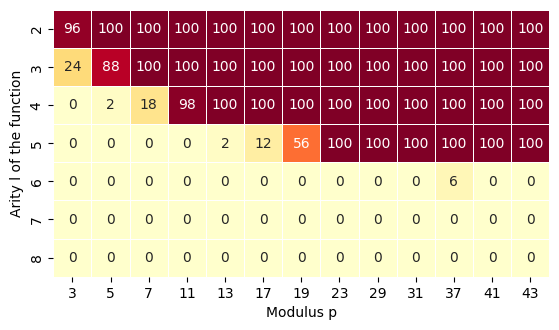
\includegraphics[]{img/p_encodings/heatmap_success.png}
    \caption{Rate of success of the algorithm for 100 random Boolean functions for different values of $\ell$ and $p$.}
    \label{fig:heatmap_success}
\end{figure}


Figure \ref{fig:lineplot_timings} shows the evolution of the time of execution of the algorithm for random Boolean functions \emph{for which no solution exists}.  It shows the explosion of the complexity for high values of
$p$, and justifies the need of a more efficient algorithm for those function (we introduce one in Section \ref{sec:graphs}).  


\TODO{Harmoniser l'algorithme suivant (commenté)}
\begin{figure}
    \centering
    \begin{minipage}{0.55\textwidth}
        \centering
        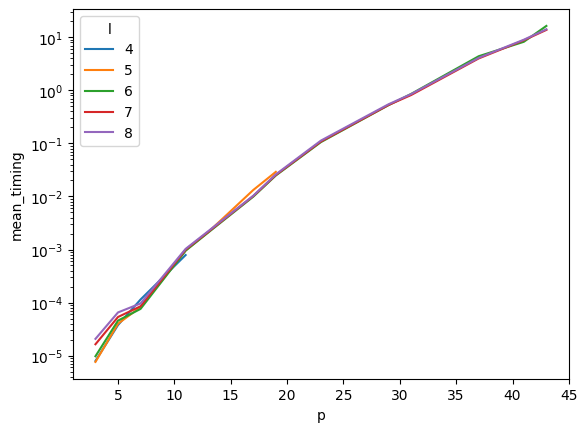
\includegraphics[width=\linewidth]{img/p_encodings/lineplot_timings.png}
        \caption{Running time of the algorithm for different values of $\ell$ and $p$ for random functions. Note that the scale is logarithmic.}        
        \label{fig:lineplot_timings}
        \end{minipage}\hspace{0.04\textwidth}
    \begin{minipage}{0.35\textwidth}
        \centering
        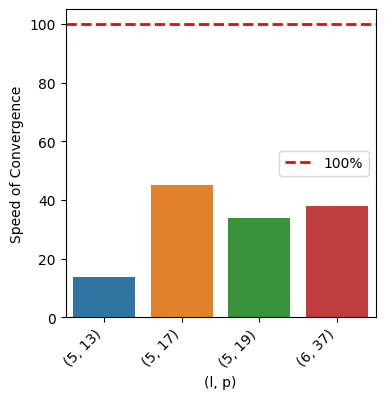
\includegraphics[width=\linewidth]{img/p_encodings/barplot.png}
        \caption{Ratio between the time to find a solution when it exists with the time to run the full algorithm when no solution exists.}
        \label{fig:barplot_ratio}
    \end{minipage}
    \caption{Some metrics about running time.}
    \label{fig:overall}
\end{figure}
Lastly, Figure \ref{fig:barplot_ratio} shows how long it takes to find a solution when one exists, relatively to the running time when no solution exist at all. It illustrates a form of "speed of convergence" and shows that it is located around $\frac{1}{3}$.



    
\subsection{An Efficient Sieving Heuristic to Find Suitable Encodings}
\label{sec:heuristic_matthieu}


Let us consider a function $f: \B^\ell \mapsto \B$ of matrix of constraints $C=(C_j^{(i)})_{\substack{1 \le i \le n_j\\1 \le j \le \ell}}$ and its associated system of linear inequalities:

$$
\left \{
\begin{array}{c}
     c_1^{(1)} \times d_1 + c_2^{(1)} \times d_2 + \dots + c_\ell^{(1)} \times d_\ell   \neq 0 \mod p\\
     c_1^{(2)} \times d_1 + c_2^{(2)} \times d_2 + \dots + c_\ell^{(2)} \times d_\ell \neq 0 \mod p\\
    \dots
\end{array}
\right .
$$


The principle is to sample random values in $\Z$ (with some large bound) and affect them to the $d_j$'s. If all the corresponding values for all the $C_i = \sum_{j=1}^{\ell} c_j^{(i)} \times d_j$ are not divisible by a value $p$, then the vector $(d_j \mod p \mid j \in \{1, \dots, \ell\})$ is a solution of the system of inequalities generated by $C$. 


To reduce the amount of samples required to find a solution, we want to avoid sampling trivially wrong sets of $d_j$'s. For example, if all the $d_j$'s are themselves divisible by $p$, then the $C_i$'s will all be divisible as well. To tackle this problem, we perform the sampling across \emph{prime numbers in $\Z$}.



%\begin{algorithm}
%    \caption{Sample a solution $\vec d$ in $\Z$ for a function $f$ and returns a possible value for $p$.}
%    \label{alg:heuristic_matthieu}
%    \begin{algorithmic}
%    \Require \\
%    $\{C_i\}_{1 \le i \le n}$ \Comment{The lines of the matrix of constraints $C$ of the function $f$ } \newline
%    $P$ \Comment{The sets of possible values for $p$ to be tested} \newline
%    $D$ \Comment{The sets of possible values in $\Z$ to assign to the $d_i$'s. All these elements are big primes}
%    \Ensure $f$ is possible to evaluate using a modulus smaller or equal than $p$.
%    \State{$\vec{d} \drawfrom D$} \Comment{Sample random prime values in $\Z$ and assign it to $\Vec{d} = (d_1, \dots, d_l)$}
%    \State{$\vec r = C \times \vec{d}$}  \Comment{$\vec r$ is the right member of the system}
%    \For {$p \in P$}
%        \If{$0 \in [\Vec{r}]_p$}          \Comment{If $p$ divides one of the coordinates of $\vec r$}
%            \State{$P \gets P \setminus \{p\}$} \Comment{This value of $p$ is incorrect}
%        \EndIf
%    \EndFor
%    \If{$\mid P \mid > 0$}
%        \State{\Return{$\min(P)$}} \Comment{Returns the smallest possible value for $p$, if any.}
%    \EndIf   
%    \end{algorithmic}
%\end{algorithm}


Running this algorithm several times and keeping the smallest returned value for $p$, one gets an upper bound on the minimum $p$ required to evaluate a function with our framework. Note that, on the contrary of the deterministic search algorithm, this heuristic does not require a prime $p$.


\paragraph{Example:} Let us consider the s-box of the block cipher ASCON. We study this s-box in more details and provide an exact optimized solution for its homomorphic evaluation in Section \ref{sec:ascon}. Here, we apply Algorithm \ref{alg:heuristic_matthieu} on the five functions generating the five output bits and monitor the results until we gather $N=10000$ non-zero possible values for $p$.


The figure \ref{fig:ascon_0_p_frequencies} shows the repartition of the returned values of $p$ by the algorithm during these $N$ runs on the first subfunction. The optimal value of $p$ found by the deterministic approach of Section \ref{sec:search_algorithm} is $17$ so the upper bound $19$ is pretty close, despite being rarely found by the algorithm. Also, the figure \ref{fig:ascon_0_count_iter} shows $21$ (the second best solution found by the sieving) is almost instantly found by the algorithm.


\begin{figure}
  \begin{minipage}{0.48\linewidth}
    \    \centering
    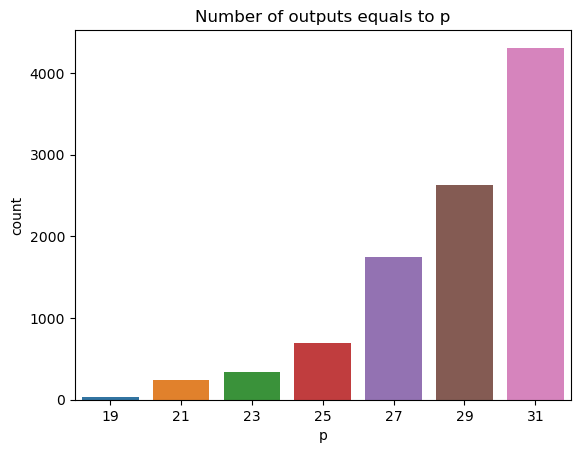
\includegraphics[width=\linewidth]{img/p_encodings/heuristic_ascon_0_p_frequencies.png}
    \caption{The outputs of $10000$ runs of the Algorithm \ref{alg:heuristic_matthieu} for the first subfunction of the Ascon s-box}
    \label{fig:ascon_0_p_frequencies}
  \end{minipage} \hfill
  \begin{minipage}{0.48\linewidth}
    \centering
    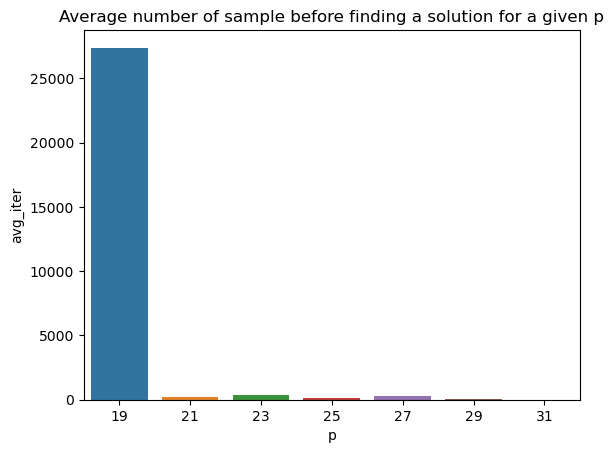
\includegraphics[width=\linewidth]{img/p_encodings/heuristric_ascon_0_count_iter.png}
    \caption{Number of iterations required to get a solution for a given value of $p$}
    \label{fig:ascon_0_count_iter}
  \end{minipage}
\end{figure}


In the process of finding the smallest $p$ possible and a correct vector of $p$-encoding to evaluate a function $f$, this heuristic is really efficient to get a tight upper bound on the value of $p$.


%\section{Scaling our Approach to any Boolean Circuit}
\label{sec:p_encodings_graphs}

Our framework optimizes the homomorphic evaluation of single Boolean functions but suffers the following limitations:

\begin{enumerate}
    \item For a Boolean function with a high number of inputs, the search algorithm may be very time-consuming.
    \item Some functions simply do not have any solution for acceptable values for $p$ ($p < 32$ for example) and thus are not efficiently evaluable in a single PBS.\footnote{The PBS can be evaluated for larger values of $p$ but it quickly becomes inefficient as $p$ grows.}
\end{enumerate}


As a consequence, we need a solution to extend our framework to these cases. In this section, we propose a strategy to leverage the circuit representation of a ``tough'' function $f$ to find a strategy of homomorphic evaluation with as few bootstrappings as possible.


\subsection{Graph of Subcircuits}
\label{sec:graph_definition}

Let $f: \B^\ell \longrightarrow \B$ be a Boolean function, and let $\mathcal{F}$ be a Boolean circuit representing $f$ (some preliminaries about Boolean circuits can be found in Section \ref{sec:p_encodings_preliminaries_boolean}). Let us describe the layout of the circuit $\mathcal{F}$. It has $\ell$ input wires, denoted by $\{y_j\}_{1 \le j \le \ell}$, and the output wire is denoted by $z$. The intermediary wires are denoted by $\{t_j\}_{1 \le j \le \theta}$. The Boolean operation gates are of fan-out 1. 


Our goal is to split the circuit into a directed acyclic graph $\mathcal{G}$, whose vertexes are subcircuits $\{\mathcal{F}_1, \dots, \mathcal{F}_k\}$ and whose edges connect the outputs of a subcircuit with the input of another. Each subcircuit $\mathcal{F}_i$ represents a subfunction $f_i: \B^{l_i} \mapsto \B$ that is evaluable with a gadget with our framework. 

We use the same notations to refer to the elements of a subcircuit $\mathcal{F}_i$ and we index them with $i$. The output of $\mathcal{F}_i$ is denoted by $z^{(i)}$ and its inputs by $\{y_j^{(i)}\}_{1 \le j \le \ell}$ and so on. 


The graph is valid for $f$ with respect to modulus $p$ if the following properties are satisfied:
\begin{itemize}
    \item Each subcircuit $\mathcal{F}_i$ has only one output $z^{(i)}$.
    \item For a subcircuit $\mathcal{F}_i$, all its inputs are either inputs of the whole circuit or outputs of other subcircuits of the graph. We can write this property as:
    $$
    \{y_j^{(i)}\}_{1 \le j \le l_i} \subset \left ( \{y_j\}_{1 \le j \le \ell} \cup \{z^{(j)}\}_{1 \le j < i} \right )
    $$
    Thus, the indexing of the $\mathcal{F}_i$'s respects the topological order of the graph, i.e. no gates of $\mathcal{F}_i$ has a child in any of the $\mathcal{F}_j$, with $j < i$.
    \item All the Boolean functions $f_i$ represented by the subcircuits $\mathcal{F}_i$ are evaluable in a single bootstrapping with modulus $p$ with our proposed method. 
    \item The last subcircuit $\mathcal{F}_c$ of the graph has $z$ (the output of the main circuit) for output: $z^{(c)} = z$.
\end{itemize}

\begin{figure}
    \centering
    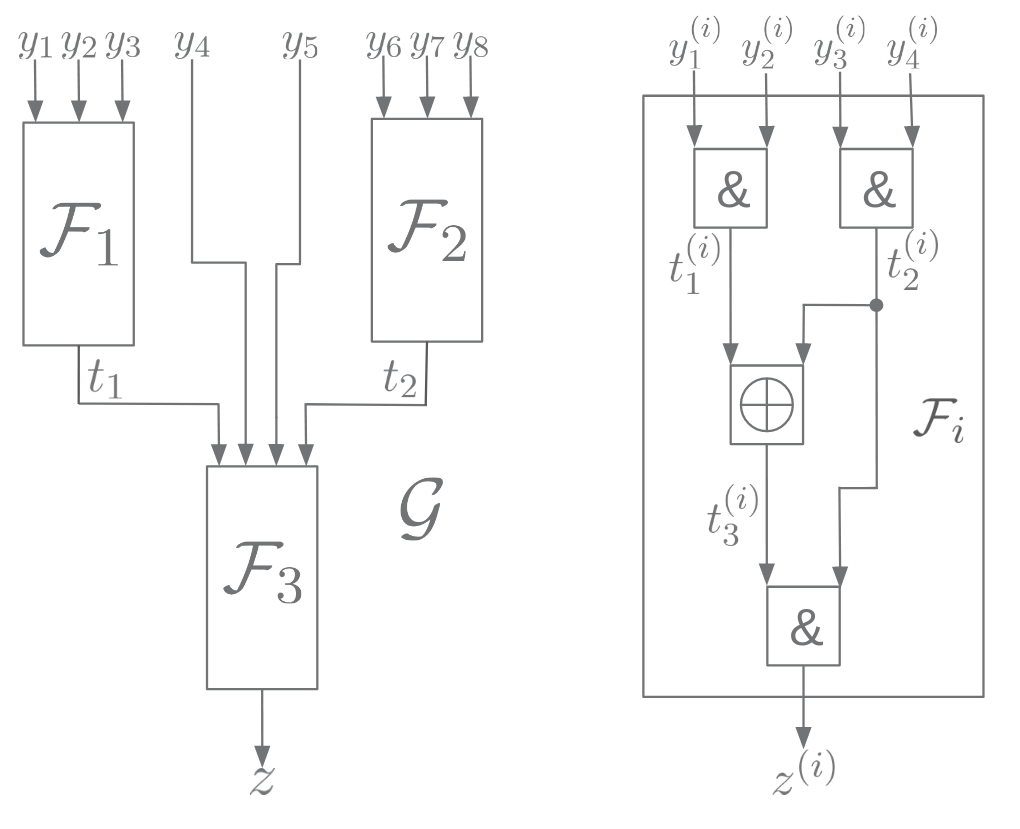
\includegraphics[width=0.75\textwidth]{img/to_harmonize/graphs.png}
    \caption{Example of graph of subcircuits (on left) and of a valid subcircuit (on right). Each subcircuit $\mathcal{F}_i$ is evaluated homomorphically with a gadget $\Gamma_i$.}
    \label{fig:enter-label}
\end{figure}




To homomorphically evaluate the function $f$, we evaluate each subcircuits with one bootstrapping for each of them and get the final result. In order to reduce the cost of evaluation for a given $p$, the goal is hence to find the \emph{smallest} valid graph possible in terms of number of subcircuits. Taking a greater value of $p$ produces a different graph that may be smaller (as subcircuits might be larger), but the timings of bootstrapping in this graph might on the other hand be greater. One can therefore run the search for different values of $p$ and keep the most efficient setup among the possible graphs. %Additionally, for some values of $p$, such a graph may not exist.

\subsection{Heuristics to Find a Small Graph}
\label{sec:heuristics_graph}

Finding such a graph can be done by exhaustively evaluating all the possible subcircuits with our method introduced in Section \ref{sec:p_encodings_search}, and then find the more efficient one. However it is not really practical to evaluate \emph{all} the possible subcircuits, so we develop some heuristics to reduce the search space. Let us start by defining a few bounds on the considered subcircuits, we will leave the other ones apart in our algorithm:

\begin{itemize}
    \item The subcircuits have at most $B$ inputs ($\forall i, l^{(i)} < B$). The purpose of this bound is to limit the running time of Algorithm \ref{alg:add_element}. In practice, for our experiments, we took $B = 10$.
    \item The subcircuits are evaluable with one single bootstrapping with a maximum value $p_{max}$. This value ensures a bootstrapping with a reasonable timing. If the search algorithm fails for $p_{max}$, the subcircuit is dropped without trying to extend $p$. In our experiment, we took $p_{max}=31$.
\end{itemize}


In order to decompose our Boolean circuit into a graph satisfying the above property for a modulus $p$, we would want to exhaustively search all the subcircuits of $\mathcal{F}$ compliant with the bounds we introduced earlier. However, all subcircuits are not equally worth to evaluate. In particular a wire incoming a copy gate is particularly worth evaluating because is costs one bootstrapping but produce several inputs for the next subcircuits. 

We gather wires that precede a copy gate in the set $\mathcal{Z}$. We add to this set the global output $z$. We also gather the input wires of the global circuit $\mathcal{F}$ in the set $\mathcal{Y}$. We define the notion of \textit{atomic subcircuit} that is a valid subcircuit whose all inputs belong to $\mathcal{Y} \cup \mathcal{Z}$ and whose output belongs to $\mathcal{Z}$. Note that the merge of two atomic subcircuits that respect the global circuit wiring is also an atomic subcircuit.

\medskip

Our heuristic works as follows:

\begin{enumerate}
    \item For each of these outputs $z_i \in \mathcal{Z}$, we exhaustively construct a set $\widehat{\mathcal{F}_{z_{i}}}$ that gathers all the atomic subcircuits whose output is $z_i$.
    We then filter out the subcircuits of $\widehat{\mathcal{F}_{z_{i}}}$ that do not comply with the bounds introduced at the beginning of the section or that are not evaluable with a gadget with the input modulus $p$ (we use Algorithm \ref{alg:add_element} to decide that).
    \medskip
    \item Now we want to construct the smallest valid graph evaluating $\mathcal{F}$ using subcircuits from the $\widehat{\mathcal{F}_{z_{i}}}$'s. While finding the smallest graph is hard, constructing any valid graph is easy. As a consequence, our strategy to find a small graph is to randomly create a lot of valid graphs and to take the smallest one. The procedure to create a valid graph is the following: we start from the output $z$ and we randomly draw a subcircuit $\mathcal{F}_z$ from $\widehat{\mathcal{F}_z}$. The inputs of $\mathcal{F}_z$ can be sorted into two categories: the ones belonging to $\mathcal{Y}$ and the ones belonging to $\mathcal{Z}$. For each one of these latter wires $w \in \mathcal{Z}$, we repeat the procedure, i.e. we draw a subcircuit $\mathcal{F}_w$ from $\widehat{\mathcal{F}_w}$, and so on. When we have reached all the input wires of $\mathcal{F}$, we get a valid graph $\mathcal{G}$ . This second step is run a large amount of times (the number of trials is a parameter of the method), and the smallest graph, i.e. the one with the fewest subcircuits, is returned.
\end{enumerate}

We carried on this method on the s-box of AES in Section \ref{sec:p_encodings_aes}.

\subsection{Parallelization of the Execution of the Graph}
\label{sec:parallelization}

Once we have our graph $\mathcal{G}$, we can identify its $n_\mathcal{L}$ \emph{layers}. Formally, they are defined as:

\begin{definition}
    A layer $\mathcal{L}$ of a graph $\mathcal{G}$ is a set of subcircuit $\{\mathcal {F}_\alpha, \dots, \mathcal{F}_\omega\}$ of $\mathcal{G}$ that verifies: $\forall \mathcal{F}_i, \mathcal{F}_j \in \mathcal{L}, \mathcal{F}_i \text{ is not an ancestor node of } \mathcal{F}_j.$    
\end{definition}

By construction, all the subcircuits belonging to the same layer can be evaluated in parallel. This reduces the number of bootstrapping steps from $k$ (the number of subcircuits in the graph $\mathcal{G}$) to $n_\mathcal{L}$ (the number of layers). Our graph-finding heuristic can be tweaked to select the graph with minimum number of layers instead of minimum number of subcircuits to optimize parallelization.

%\section{Adaptation of TFHE and the \texttt{tfhe-rs} Library}
\label{sec:TFHE_adaptation}

From a high level point of view, our technique can be seen as adding an additional layer of abstraction on top of TFHE. However things are not that simple: picking odd values for $p$ leads to some changes in the inner working of the programmable bootstrapping (PBS), and the choice of parameters is also affected by this change. Moreover, we implemented our framework by forking the \texttt{tfhe-rs} library~\cite{tfhe-rs} written in Rust. The following section covers the adaptation of the PBS and the choice of new parameters. The adaptation of the library is treated in Section \ref{sec:library}.

\subsection{Dealing with the Negacyclicity Problem for an Odd $p$}
\label{sec:solving_negacyclicity}

In the following, we explain the negacyclicity problem and how we propose to solve it. To do so, we need to dig into the details of the \texttt{BlindRotate} step of the PBS, that we have introduced in Section \ref{sec:bootstrapping}.

Let $v(X)$ be a polynomial of the ring $\Z_{q, N}[X]/(X^N+1)$, denoted by $v(X) = \sum_{k=0}^{N-1} v_k X^k$. Observe that a multiplication by $X$  in this ring ``rotates'' the coefficients of the polynomial: \[X \cdot v(X) = - v_{N - 1} + v_0 \cdot X \dots + v_{N - 2} X^{N - 1}~.\]

In TFHE, the polynomial multiplication in the blind rotation is actually done by $X^{-\Tilde{\mu}}$, with $\Tilde{\mu} = \rounding{\frac{\mu \cdot 2N}{q}}$, which lives in $\{0, \dots, 2N - 1\}$. This leads to two problems:

\begin{itemize}
    \item A coefficient $v_j$ can be brought in first place by two differents rotations: the one induced by the polynomial multiplication by $X^{\modulo{-j}{2N}}$ and the one by $X^{[-j + N]_{2N}}$.
    \item Each time a coefficient goes last to first, it gets negated (because $X^N = -1$ in the ring). So actually, the multiplication by $X^{[-j]_{2N}}$ yields correctly $v_j$, but the one by $X^{[-j + N]_{2N}}$ yields $-v_j$.
\end{itemize}


However, these problems can be circumvented for even and odd values of $p$. Recall that $\mu = m + e \in \Z_q$, with $e$ sampled from a small centered Gaussian. The use of a small error makes that $\mu$ does not take all the values of $\Z_q$ with the same probability: in particular, the densest parts in terms of probability over $\Z_q$ are the one close to the ``unscrambled'' values of $m$, namely $\left \{ \rounding{\frac {k q}{p}} \mid k \in \Z_p \right \}$. We illustrate this distribution on Figure \ref{fig:density_of_phase}. We call these sections of the torus the \emph{dense spots}.


\begin{figure}
    \begin{subfigure}{0.49\linewidth}
        \centering
        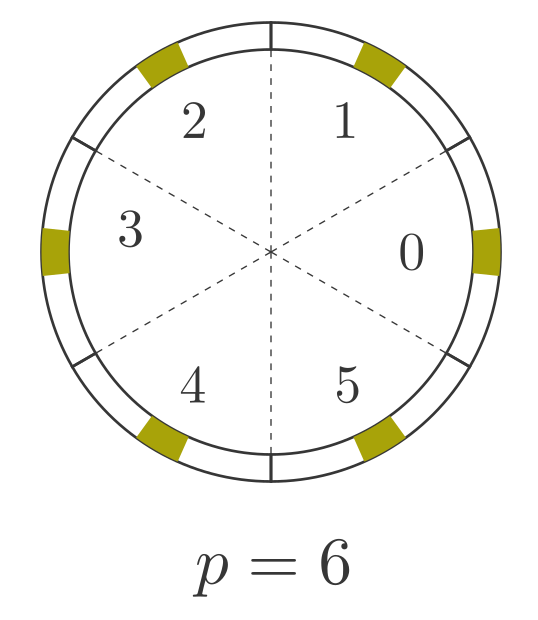
\includegraphics[width=0.5\linewidth]{img/to_harmonize/busy_sectors_2.png}
    \end{subfigure}\hspace{1em}% Adjust the margin width as needed
    \begin{subfigure}{0.49\linewidth}% Specify the width here
        \centering
        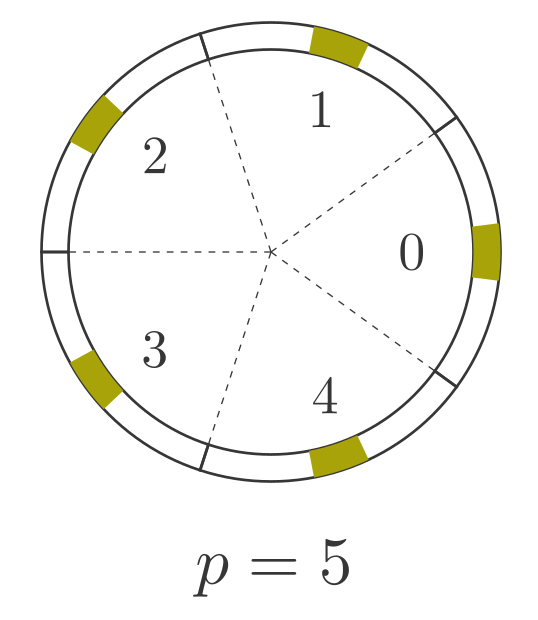
\includegraphics[width=0.5\linewidth]{img/to_harmonize/busy_sectors.png}
    \end{subfigure}
    \caption{Distribution of the values of $\mu$ across $\Z_{q}$ for $p = 6$ and $p = 5$: the colored parts show the dense spots where the value has a high probability to lie in. The width of these sectors depends on $\sigma$ (the standard deviation of the error distribution $\chi$ of TFHE). Note that this repartition looks the same for $\Tilde{\mu}$ in $\Z_{2N}$.}    
    \label{fig:density_of_phase}
\end{figure}


When we transpose these dense spots into $\Z_{2N}$, they become the sectors close to $\left \{ \rounding{\frac{k \cdot 2N}{p}} \mid k \in \Z_p \right \}$. Let us note that the noises in $\Z_q$ and $\Z_{2N}$ are fundamentally different: the former is the one added at encryption that may have grew during the homomorphic computations, and the latter is called ``drift'' and is caused by the accumulation of the rounding errors on each coefficient of the ciphertext during the modulus switching (but this difference in nature does not impact our purpose). 
Let $k \in \Z_p$, the multiplication $X^{- \frac{k \cdot 2N}{p}} \cdot v(X)$ yields the same degree-zero coefficient as the multiplication  $X^{\modulo{- \frac{k \cdot 2N}{p} + N}{2N}} \cdot v(X)$, up to the minus sign. For the sake of clarity, we write the exponent of the latter in a slightly different manner: 
\[\modulo{
    \frac{
        -k \cdot 2N
        }
    {
        p
    }
    + N
}{2N} = 
\modulo{
    \frac{
    (-k + \frac p 2 ) \cdot 2N
    }
    {p}
}
{2N}\]


This is where the parity of $p$ plays a part: if $p$ is even, then $\modulo{
    \frac{
    (-k + \frac p 2 ) \cdot 2N
    }
    {p}
}
{2N}$ is a dense spot as well. So, the rotations by these two values will happen with high probability and they will both yield the same coefficient $v_{\frac{k \cdot 2N}{p}}$ (up to the minus sign for one of them). Thus, when evaluating a function $f$ with a PBS, the calls $f(k)$ and $f(k + \frac p 2)$ will produce the same output (one again, up to the minus sign), which is a collision constraining the definition of $f$. On the other hand, let us consider an odd value for $p$. Then, $\modulo{
    \frac{
    (-k + \frac p 2 ) \cdot 2N
    }
    {p}
}{2N}$ is no longer a dense spot, as it lies exactly halfway between the two dense spots $\modulo{
    \frac{
    (-k + \frac {p-1} {2} ) \cdot 2N
    }
    {p}
}{2N}$ and $\modulo{
    \frac{
    (-k + \frac {p+1} {2} ) \cdot 2N
    }
    {p}
}{2N}$. As a consequence, collision never occurs. Figure \ref{fig:torus_p_even_vs_odd} illustrates this phenomenon.


\begin{figure}
  \begin{subfigure}{0.49\linewidth}
    \    \centering
    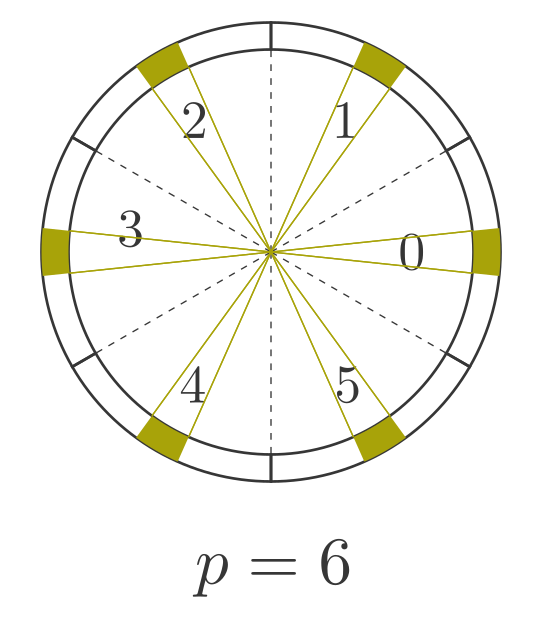
\includegraphics[width=0.5\linewidth]{img/to_harmonize/torus_p_even.png}
    \caption{With $p$ even, the dense spots of each half of the torus are aligned.}
    \label{fig:torus_p_even}
  \end{subfigure}\hspace{1em}% Adjust the margin width as needed
  \begin{subfigure}{0.49\linewidth}
    \centering
    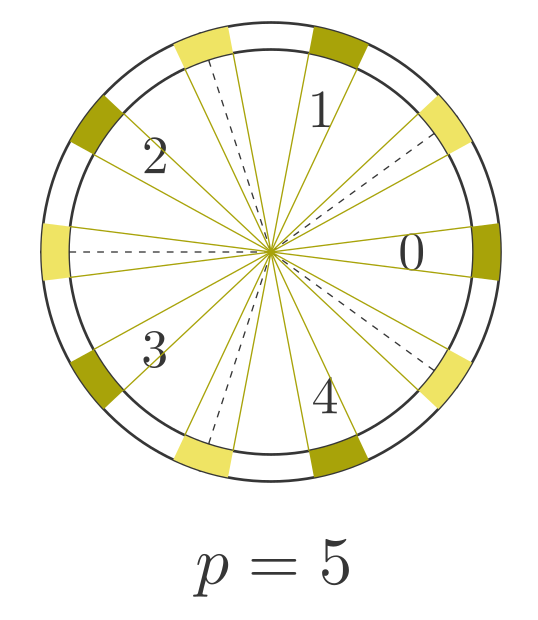
\includegraphics[width=0.5\linewidth]{img/to_harmonize/torus_p_odd.png}
    \caption{With $p$ odd, the dense spots face empty spots, close to the bounds of the $p$-sectors.}
  \end{subfigure}
  \caption{}
  \label{fig:torus_p_even_vs_odd}
\end{figure}



That is why we select only odd values for $p$ in our framework. 


We will see in Section \ref{sec:parametrization} how this change impacts the parametrization of the scheme.

\TODO{Ecrire que ça ne chanre rien au paramétrage, avec une référence sur la bonne section}






\paragraph{Exception for $p=2$:} We just said that only odd values can be selected for $p$ in our framework, however $p$-encodings with even values of $p$ exist as well: nonetheless they need to achieve the relaxed negacyclicity property introduced in Definition \ref{def:encoding}. This restriction makes them basically useless, as using only odd $p$-encodings is sufficient to evaluate all possible Boolean functions without having to bother with the negacyclicity property. However, the case $p=2$ is an exception: the valid $2$-encodings are automatically negacyclic and allow to evaluate the \texttt{XOR} operation by simply performing an homomorphic sum (so without bootstrapping). So it might be efficient to switch between $2$-encodings for \texttt{XOR} operations and $p$-encodings (with odd $p$) for non-linear Boolean functions. We make use of this strategy in our implementation of the Keccak permutation in Section \ref{sec:keccak} and for the AES in Section \ref{sec:aes}.



\subsection{Construction of the Accumulator for an Odd $p$}
\label{sec:accumulator}


The accumulator is the polynomial $v(X)$ used in the \texttt{BlindRotate} step of the PBS. In the Section \ref{sec:solving_negacyclicity}, we showed how the values are spread over the torus after bootstrapping. To actually make that works, we need to explicitly characterize this polynomial. In the following presentation, we neglect roundings to keep notations light (as if $p$ would divide $N$), or, equivalently, the division operator is assumed to include rounding.

\begin{definition}
    If $p$ is an odd modulus, and $f: \Z_p \mapsto \Z_{p'}$ a function, then the accumulator $v(X) \in \Z_{N, q}[X]/(X^N+1)$ has the form:\[v(X) = X^{- \frac {N} {2p}} \cdot \sum_{j=0}^{N/p - 1} X^j  \cdot \left ( \sum_{i=0}^{\frac{p-1}{2}} f(i) X^{i \frac{2N}{p}} + \sum_{i=0}^{\frac{p-1}{2} - 1} -f \left (i + \frac{p+1}{2} \right ) X^{i \frac{2N}{p} + \frac N p} \right )\]
\end{definition}


Let us explain the structure of this accumulator. The polynomial has degree $N$ and is made of $p$ distinct windows of width $\frac{N}{p}$. Each of these windows has constant coefficient value $f(k)$, for $k \in \{0, \dots, p-1\}$.
For $0 \le \alpha \le \frac{p-1}{2}$, the range of degrees whose coefficients are $f(\alpha)$ is $\left [ \alpha \frac{2N}{p} - \frac{N}{2p}~;~ \alpha \frac{2N}{p} + \frac{N}{2p} \right ]$. Now, for $\frac{p+1}{2} \le \beta \le p-1$, we can write $\beta = \alpha + \frac{p+1}{2}$, with $0 \le \alpha < \frac{p-1}{2}$. This time, the range of spanned degrees is $\left [ \alpha \frac{2N}{p} + \frac{N}{2p} ~;~ (\alpha + 1) \frac{2N}{p} - \frac{N}{2p} \right ]$. Thus, the values $k \in \{0, \dots, p-1\}$ spans the entire space $[0; N)$ without overlap. The values over $\frac{p+1}{2}$ gets negated by the negacyclicity, so the underlying coefficient is also negated to compensate this effect. We illustrate this construction on Figure \ref{fig:accumulator}.

\begin{figure}
    \centering
    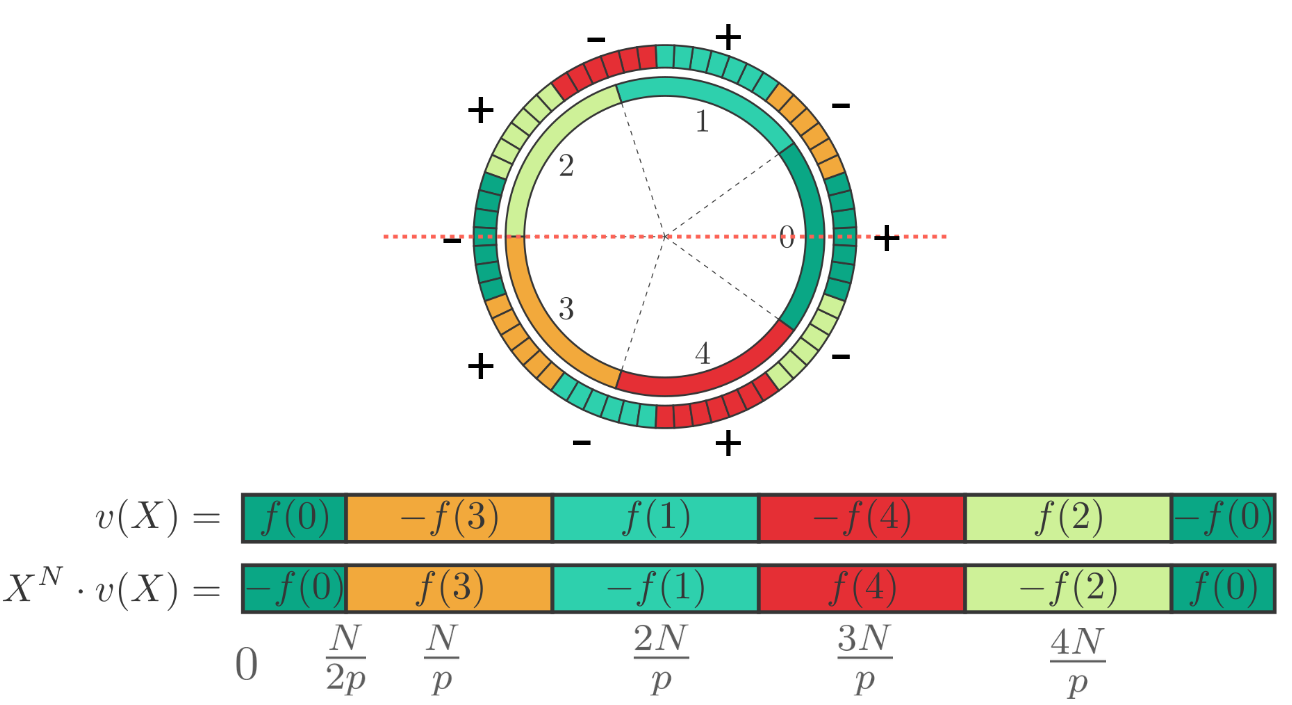
\includegraphics[width=\textwidth]{images/accumulator.png}
    \caption{Illustration of the construction of the accumulator. On top is the ring $\Z_{2N}$ splitted in windows. Below is a representation of the polynomial $v$, with its version once rotated by a multiplication by $X^N$. On the figure, $p$ = 5.}
    \label{fig:accumulator}
\end{figure}



\subsection{Crafting of Parameters}
\label{sec:parametrization}
The instances of the TFHE scheme are defined by a set of parameters. These parameters should simultaneously ensure the security of the scheme and the correctness of the homomorphic computations. They also determine the time of execution of one PBS. Here we define a framework to dimension the parameters required to optimally execute a given gadget.

Finding an optimal set of parameters for a given application is a hard problem and has been studied in particular in \cite{zama_parameters_optimization}. The parameters need to ensure three properties: security, correctness and efficiency. 

Let us start by an overview of the different parameters at play in an instance of the TFHE bootstrapping:

\begin{itemize}
    \item $n$: the dimension of the \LWE samples. Namely, the TLWE ciphertexts are vectors of length $n + 1$.
    \item $q$: the modulus of the ring the encrypted values live on. In \texttt{tfhe-rs} those values are stored on \texttt{u32} values, making $q = 2^{32}$. We treat this as an immutable platform-dependent value.
    \item $\sigma$: the standard deviation of the Gaussian distribution of error in \LWE samples.
    \item $k$: the dimension of the \GLWE samples. If $k=1$, we talk about \RLWE samples.
    \item $\sigma'$: the standard deviation of the Gaussian distribution of error in \GLWE samples.
    \item A few more parameters dimensioning some inner algorithms of the bootstrapping. A detailed description and an analysis of their impact on performances and noise level can be found in \cite{zama_parameters_optimization}. In this work, they are denoted as \emph{micro-parameters}.
\end{itemize}

In \cite{zama_parameters_optimization}, authors elaborate a strategy where they define an \textit{atomic pattern} of FHE operators, that is to say a subgraph of FHE operators in which the noise of the output is independent from the one in the inputs. Then, they develop an optimization framework to derive the best set of parameters for a given atomic pattern.

In particular, the first atomic pattern they study, that they denote by $\mathcal{A}^{(CJP21)}$, is a subgraph composed of a linear combination of ciphertexts with clear constants, then a \texttt{Keyswitch} and then a \texttt{BlindRotate} followed by a \texttt{SampleExtract} (\texttt{ModulusSwitch} is seen as a part of \texttt{BlindRotate}). Note that in Section \ref{sec:bootstrapping} we introduced the bootstrapping of TFHE by putting the \texttt{BlindRotate} before the \texttt{Keyswitch}, but the other way around is also doable. To dimension the parameters of TFHE to evaluate such an atomic pattern, their framework takes as input the 2-norm of the vector of constants of the linear combination (denoted by $\nu$) and a noise bound $t$ on the standard deviation of the distribution of error in a ciphertext that ensures a correct decryption with a good probability $(1-\epsilon$). We elaborate further on how this bound is constructed below in this section.

If we look closely, the evaluation of a gadget we introduced in Definition \ref{def:gadget} can be seen as a $\mathcal{A}^{(CJP21)}$ with a few differences. Thus, we slightly modified the tool \texttt{concrete-optimizer} \cite{concrete-optimizer}, that allows to generate parameters for different types of atomic patterns, to support our gadget as a new atomic pattern. Let us dive into the differences between a gadget and a $\mathcal{A}^{(CJP21)}$:

\paragraph{Support of odd values for $p$:} Using an odd value for $p$ changes the bootstrapping procedure, and in particular the definition of the accumulator for the \texttt{BlindRotate} (as explained in Section \ref{sec:accumulator}). With our construction, the windows in the polynomial are half the size of the ones for an even $p$, which impacts the noise bound $t$. 
As this bound depends of the failure probability $\alpha$ that the user is ready to tolerate, we shall denote it $t_\alpha$ hereafter, which satisfies: $t_\alpha = \frac{\Delta}{2z^*(1-\sqrt[N]{1-\alpha})}$
where $z^*$ is the \emph{standard score} and $\Delta$ is the scaling factor (see~\cite{zama_parameters_optimization} for more explanations). The impact of our adaptation on this formula is solely with respect to the scaling factor. In the context of an $\mathcal{A}^{(CJP21)}$, we have $\Delta = \frac{q}{2^\pi p}$ with $\pi$ the number of MSB for padding. As explained in Section \ref{sec:solving_negacyclicity}, we do not need any padding mechanism anymore, so the $2^\pi$ vanishes. However, the length of a window is divided by $2$, and $p$ does not divide $q$ anymore so we need to add a rounding. We finally get $\Delta = \rounding{\frac{q}{2p}}$.


\paragraph{Link between input encodings and $\nu$:} In a scenario where only one gadget has to be evaluated, its inputs are freshly encrypted ciphertexts. Then, there is no need to perform any encoding switching before evaluating the gadget, and so we are in the context of a $\mathcal{A}^{(CJP21)}$ with $\nu = 1$. However, if we are in a context of a \textit{graph} of gadgets like in Section \ref{sec:graphs}, the output of a gadget can be used as input of subsequent gadgets under different encodings. In this case, some encoding switchings are necessary. If these encoding switching are made using a mutiplication by a constant (Property \ref{prop:mult_constant}), we are still in the context of a $\mathcal{A}^{CJP21}$ but with $\nu \ne 1$. 
To formalize that, we first recall that Algorithm \ref{alg:add_element} produces gadgets of the form $\Gamma = \left (\vec{\Encoding_{in}}, \Encoding_{out}, p_{in}, p_{out}, f \right )$, with $\Encoding_{in}^{(i)} = \EncDefOne{d_i}$. Thus, if we fix that all gadget output ciphertexts are encoded under $\Encoding_{out} = \EncDefOne{1}$, then the encoding switchings needed before an evaluation of $\Gamma$ corresponds to a linear combination of the inputs with the vector $\vec d = (d_i \mid i \in [1, \ell])$, so we fall back on a $\mathcal{A}^{(CJP21)}$ with $\nu = \customnorm{\vec d}$.


We implemented these changes in \texttt{concrete-optimizer} and uses it to generate sets of parameters for our implementations detailed in Section \ref{sec:implementations}.

\subsection{Concrete Implementations of $p$-Encodings and Homomorphic Functions in \texttt{tfhe-rs}}
\label{sec:library}


To implement our framework, we relied on the $\texttt{tfhe-rs}$ library~\cite{tfhe-rs}. Here is a list of the major changes we applied to the code:

\paragraph{Addition of the notion of $p$-encoding: } An encoding $\Encoding$ is simply implemented with a structure \texttt{Encoding} storing two \texttt{HashSets} and the modulus $p$. The \texttt{HashSets} represent both sets $\Encoding(0)$ and $\Encoding(1)$. When creating an \texttt{Encoding}, the code checks whether the two underlying sets are disjoint or not. Moreover, the operation of encryption and decryption are modified as well. The signatures change from:\[\texttt{encrypt(Boolean, ClientKey) -> Ciphertext}\] to: \[\texttt{encrypt(Boolean, ClientKey, Encoding) -> Ciphertext}\] (same for \texttt{decrypt}). The functions also perform the mapping $\B \mapsto \Z_p$ before encryption and the other way around after decryption.


\paragraph{Support of odd moduli: } The native \texttt{tfhe-rs} only support power-of-two-moduli $p$. We extended the library to handle odd values for $p$. This required modifying the encryption and decryption algorithm, and to compute the sets of parameters with the method of Section \ref{sec:parametrization}.


\paragraph{Definition of the new structure $\texttt{Gadget}$: } According to the evaluation strategy we introduced in Section \ref{sec:new_strategy}, we wrote a new structure $\texttt{Gadget}$, associated to a Boolean function $f: \B^\ell \mapsto \B$, carrying:
\begin{itemize}
    \item A list of the \texttt{Encoding} objects for the inputs: $\Encoding_{in} = (\Encoding_1, \dots, \Encoding_l)$, with the input modulus $p_{in}$ they encoded on.
    \item The output \texttt{Encoding} object $\Encoding_{out}$, with the output modulus $p_{out}$ it is encoded on.
    \item The clear function $f$.
\end{itemize}
When such a structure is constructed, it self-checks whether $f(\Encoding_{in})$ is valid. Then, when provided $\ell$ $\texttt{Ciphertexts}$ objects encoded under their respective $p$-encoding, it executes the homomorphic sum and the PBS and outputs the results encoded under $\Encoding_{out}$. Some utilitary functions performing encoding-switching are also available, allowing the chaining of several $\texttt{Gadget}$.


\paragraph{Implementation of the accumulator: } The procedure of bootstrapping of \texttt{tfhe-rs} is slightly modified to support the new version of the accumulator we introduced in Section \ref{sec:accumulator}.

\paragraph{Parsing of graphs: } We implemented a Python script that produces graphs to represent more complex functions that requires several PBS, as described in Section \ref{sec:graphs}. These graphs are stored with a comprehensive file format and our Rust implementation has a module of parsing allowing to load these graphs and automatically generate the corresponding graph of \texttt{Gadget}.




%
\section{Application to Cryptographic Primitives}
\label{sec:p_encodings_implementations}


In this section, we apply our approach on some cryptographic primitives. For each primitive, we first explain the construction of the gadgets required and report the concrete performances of our implementation. We detailed all the timings of our experimentations along with the sets of parameters we used in Section \ref{sec:tables_perfs}.

For performance measurement, we implemented our framework in our fork of the library \texttt{tfhe-rs} \cite{tfhe-rs} adapted as discussed in Section \ref{sec:TFHE_adaptation} and we generated the sets of parameters thank to our version of \texttt{concrete-optimizer} \cite{concrete-optimizer}. By default, we tailored the sets of parameters to limit the probability of failure $\epsilon$ of a bootstrapping to $2^{-40}$, and a security level of $\lambda = 128$ bits. All experiments have been carried out on a laptop with a 12th Gen Intel(R) Core(TM) i5-1245U CPU with 10 cores and a frequency of 4.4 GHz, and 16 GB of RAM.


\subsection{SIMON Block Cipher}
\label{sec:simon}

SIMON is a hardware-oriented block cipher developed in \cite{simon}, which relies only on the following operations: \texttt{AND}, rotation, \texttt{XOR}. It is a classical Feistel network for which the Feistel function consists in applying basic operations on the branch, xoring the subkey and then xoring the result with the other branch as depicted in the Figure~\ref{fig:simon_cipher} (on this figure, $S^i$ denotes the left circular shift by $i$ bits.). We use one ciphertext per bit so the rotation operation is essentially free. Note that the key is considered as a plaintext, which does not change anything in the framework. In our implementation, we considered a (128-128) instance of SIMON (i.e. the whole state and the key are of size 128). 


% \begin{wrapfigure}{r}{5.5cm}
% 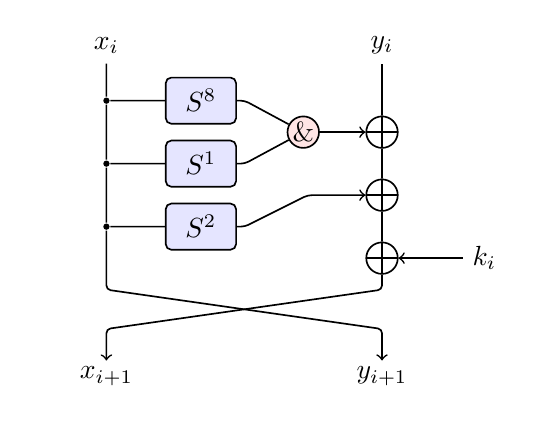
\begin{tikzpicture}
  [line width=0.6,trim left,
   shiftbox/.style = {
     draw, fill=blue!10, rounded corners=2pt,
     inner xsep=0.25cm, inner ysep=0.15cm,
   },
   wire/.style = {
     rounded corners=1.5pt
   },
   xor/.style = {
     draw, circle, inner sep=0cm, minimum size=0.4cm,
     append after command = {
       [shorten >=\pgflinewidth, shorten <=\pgflinewidth,]
       (\tikzlastnode.north) edge (\tikzlastnode.south)
       (\tikzlastnode.east) edge (\tikzlastnode.west)
     }
   },
   odot/.style = {
     draw, circle, inner sep=0cm, minimum size=0.4cm,fill=red!10
   },
   dot/.style = {
     fill, circle, inner sep=0cm, minimum size=0.08cm
   }]

  %Draw nodes
  \node at (1,6.7) (xin) {$x_i$};
  \node at (4.5,6.7) (yin) {$y_i$};
  \node[dot] at (1,6) (d1) {};
  \node[dot] at (1,5.2) (d2) {};
  \node[dot] at (1,4.4) (d3) {};
  \node[shiftbox] at (2.2,6) (S1) {$S^8$};
  \node[shiftbox] at (2.2,5.2) (S2) {$S^1$};
  \node[shiftbox] at (2.2,4.4) (S3) {$S^2$};
  \node[xor] at (4.5,5.6) (x1) {};
  \node[xor] at (4.5,4.8) (x2) {};
  \node[xor] at (4.5,4.0) (x3) {};
  \node[odot] at (3.5,5.6) (AND) {\&};
  \node at (5.8,4.0) (k) {$k_i$};
  \node at (1, 2.5) () {$x_{i+1}$};
  \node at (4.5, 2.5) () {$y_{i+1}$};

  %Draw wires
  \draw[wire] (d1) -- (S1)  (S1.east) -- +(0.1,0) -- (AND);
  \draw[wire] (d2) -- (S2)  (S2.east) -- +(0.1,0) -- (AND);
  \draw[wire,->] (AND) -- (x1);
  \draw[wire,->] (d3) -- (S3) (S3.east) -- +(0.1,0) -- ++(0.9,0.4) -- (x2);
  \draw[wire,->] (xin) -- (d1) -- (d2) -- (d3)
                  -- ++(0,-0.8) -- ++(3.5,-0.5) -- ++(0,-0.4);
  \draw[wire,->] (yin) -- (x1) -- (x2) -- (x3)
                 -- ++(0,-0.4) -- ++(-3.5,-0.5) -- ++(0,-0.4);
  \draw[wire,->] (k.west) -- (x3);
\end{tikzpicture} 
%    \caption{One Feistel round of SIMON. }   
%    \label{fig:simon_cipher}
% \end{wrapfigure}

\begin{figure}
    \centering
    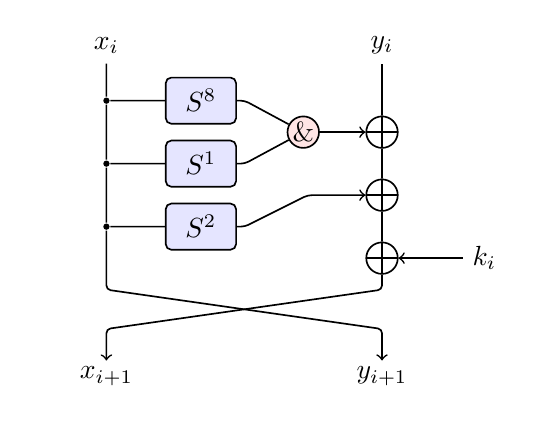
\begin{tikzpicture}
  [line width=0.6,trim left,
   shiftbox/.style = {
     draw, fill=blue!10, rounded corners=2pt,
     inner xsep=0.25cm, inner ysep=0.15cm,
   },
   wire/.style = {
     rounded corners=1.5pt
   },
   xor/.style = {
     draw, circle, inner sep=0cm, minimum size=0.4cm,
     append after command = {
       [shorten >=\pgflinewidth, shorten <=\pgflinewidth,]
       (\tikzlastnode.north) edge (\tikzlastnode.south)
       (\tikzlastnode.east) edge (\tikzlastnode.west)
     }
   },
   odot/.style = {
     draw, circle, inner sep=0cm, minimum size=0.4cm,fill=red!10
   },
   dot/.style = {
     fill, circle, inner sep=0cm, minimum size=0.08cm
   }]

  %Draw nodes
  \node at (1,6.7) (xin) {$x_i$};
  \node at (4.5,6.7) (yin) {$y_i$};
  \node[dot] at (1,6) (d1) {};
  \node[dot] at (1,5.2) (d2) {};
  \node[dot] at (1,4.4) (d3) {};
  \node[shiftbox] at (2.2,6) (S1) {$S^8$};
  \node[shiftbox] at (2.2,5.2) (S2) {$S^1$};
  \node[shiftbox] at (2.2,4.4) (S3) {$S^2$};
  \node[xor] at (4.5,5.6) (x1) {};
  \node[xor] at (4.5,4.8) (x2) {};
  \node[xor] at (4.5,4.0) (x3) {};
  \node[odot] at (3.5,5.6) (AND) {\&};
  \node at (5.8,4.0) (k) {$k_i$};
  \node at (1, 2.5) () {$x_{i+1}$};
  \node at (4.5, 2.5) () {$y_{i+1}$};

  %Draw wires
  \draw[wire] (d1) -- (S1)  (S1.east) -- +(0.1,0) -- (AND);
  \draw[wire] (d2) -- (S2)  (S2.east) -- +(0.1,0) -- (AND);
  \draw[wire,->] (AND) -- (x1);
  \draw[wire,->] (d3) -- (S3) (S3.east) -- +(0.1,0) -- ++(0.9,0.4) -- (x2);
  \draw[wire,->] (xin) -- (d1) -- (d2) -- (d3)
                  -- ++(0,-0.8) -- ++(3.5,-0.5) -- ++(0,-0.4);
  \draw[wire,->] (yin) -- (x1) -- (x2) -- (x3)
                 -- ++(0,-0.4) -- ++(-3.5,-0.5) -- ++(0,-0.4);
  \draw[wire,->] (k.west) -- (x3);
\end{tikzpicture} 
    \caption{One Feistel round of SIMON. }     
    \label{fig:simon_cipher}
\end{figure}


The Boolean function to evaluate can be defined as $$f(b_0, b_1, b_2, b_3, b_4) = b_0 \cdot b_1 \oplus b_2 \oplus b_3 \oplus b_4~.$$


Using Algorithm \ref{alg:add_element}, we found the smallest possible $p$ ($p = 9$) and the following $9$-encodings to evaluate each bit of the Feistel function with one single bootstrapping (i.e. totalling 64 PBS per round). 


\[\Encoding_0 = \Encoding_1 = \EncDefOne{1} \text{ and } \Encoding_2 = \Encoding_3 = \Encoding_4 = \EncDefOne{2} \text{ with } p = 9.\] The sum of these $p$-encodings yields the output encoding: \[\Encoding_{out} = \EncDef{\{0, 1, 4, 5, 8\}}{\{2, 3, 6, 7\}} \text{ with } p=9\] which is valid for $f$. After the PBS, all the bits of the state are encrypted under the encoding $\Encoding_0$. We formalize that with the gadget $\Gamma = \left ((\Encoding_0, \Encoding_1, \Encoding_2, \Encoding_3, \Encoding_4), \Encoding_0, 9, 9\right )$


To perform a Feistel round on a state of size $k$, the gadget $\Gamma$ is applied in parallel $k / 2$ times. Note that one bit may be used in several evaluation as $b_0$, $b_1$ and $b_2$. So we sometimes have to switch from $\Encoding_0$ to $\Encoding_1$ by a simple external multiplication by $2$, which is negligible in terms of performances.


Using our version of \texttt{concrete-optimizer} \cite{concrete-optimizer}, we crafted a set of parameters suitable for this modulus and these encodings. 
On our machine, one PBS with such parameters takes about $9.5$ ms. The theoretical timings achieved on one full block without any parallelization is $41$ seconds ($68$ rounds $\times$ $64$ bits $\times$ $9.5$ ms)  which we confirmed experimentally.


Nonetheless, this setting is intrinsically parallelizable: the 64 gadgets of each round can be performed in parallel. We implemented parallelization using the module \texttt{Rayon} of Rust, which made the total timings drop to $13$ seconds on our machine. 

Compared to \cite{DBLP:conf/fps/BendoukhaSSQS22} that implemented the same block cipher on an equivalent hardware with parallelism, our implementation is about 10 times faster. Table \ref{tab:concrete_perfs} shows the comparison. Note that in this paper, the probability of failure is not specified. As ours is pretty conservative, this is a good argument in favor of our framework.


\subsection{The Trivium Stream Cipher}
\label{sec:trivium}

Trivium \cite{ISC:DeCanniere06} is a stream cipher that uses a circular state. At each round, the bits are rotated within the state, except for three of them that are refreshed using the Boolean function of Section \ref{sec:simon}. The outer stream is generated by xoring three bits of the state each round once a ``warming-up'' phase is achieved. 


For each generated key bit, it requires performing this function three times and aggregating five \texttt{XOR} operations in the center. Our strategy is to evaluate the refreshing function three times per round with one PBS for each of them, then get the result in $\Z_2$ and chain the five \texttt{XOR} operations to get the output.
Figure \ref{fig:triviuml} illustrates the layout of the cipher.
\begin{figure}
    \centering
    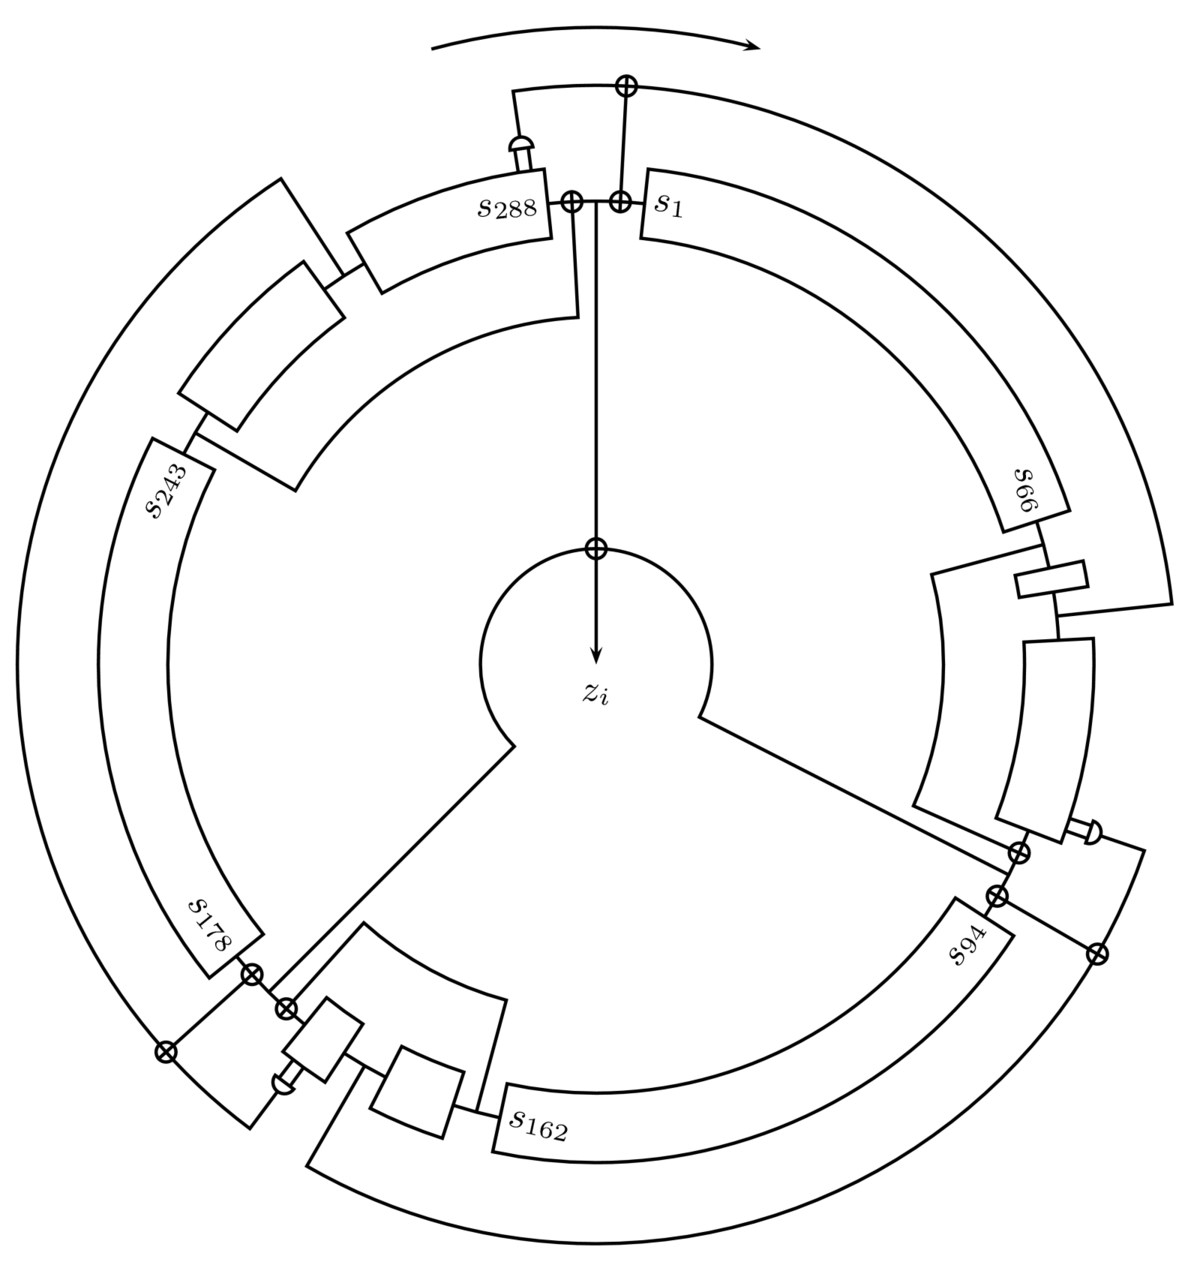
\includegraphics[width=0.5\linewidth]{img/to_harmonize/trivium.png}
    \caption{The trivium stream cipher. Figure extracted from \cite{ISC:DeCanniere06}}.
    \label{fig:triviuml}
\end{figure}


In \cite{DBLP:conf/wahc/BalenboisOS23}, the authors implement Trivium using the original \texttt{tfhe-rs} library, with 2 bits of message and 2 bits of carry for a total of 4 significative bits out of the 32 of a ciphertext component. They call this mode the \texttt{shortint} mode. The use-case they target is transciphering.

To compare our implementation with the one of \cite{DBLP:conf/wahc/BalenboisOS23}, timings are not a good metric as in their work they are provided on a massive AWS instance with a significant amount of parallelism. A better metric is to count the number of PBS and compare the parameter sets.

We reproduced the PBS operation with their parameter set on our machine and then simply estimated the timings of one round of Trivium with their approach with no parallelism. The results are summed up in Table \ref{tab:perfs_trivium}. Note that in our implementation we do not refresh the output bits with a PBS after the chain of \texttt{XOR}, because in the use-case of transciphering one more \texttt{XOR} has to be performed with the message. We take advantage of this and move the last PBS into the transciphering phase.

\begin{table}[htbp]
\centering
\caption{Comparison of timings of one round of Trivium between our work and \cite{DBLP:conf/wahc/BalenboisOS23}, with $\epsilon=2^{-40}$.}
\label{tab:perfs_trivium}
\begin{tabular}{|c|c|c|c|}
\hline
Instance & Timing PBS & Number of PBS per round & Estimated timings \\
\hline
\cite{DBLP:conf/wahc/BalenboisOS23} & 6.6 & 7 & 46.2 ms \\
\hline
Our work & 9.5 & 3 & 28.5 ms \\
\hline
\end{tabular}
\end{table}

\subsection{Keccak Permutation}
\label{sec:keccak}

Keccak is a hash function standardized by NIST under the name \emph{SHA-3} \cite{sha-3}. It is a sponge function, whose transformation is called the \emph{Keccak permutation}. It consists of five sub-functions: $\theta$, $\rho$, $\pi$, $\chi$, and $\iota$.

Let us recall that our approach encrypts each bit in one TFHE ciphertext. Let us explain the stategies of homomorphization of these sub-functions:
\begin{itemize}
    \item $\rho$ and $\pi$ simply reorder the bits within the state, so they are not impacted by the homomorphization.
    \item $\theta$ is just a serie of \texttt{XOR} operations, so it can be performed with a serie of homomorphic additions and without any PBS provided that the input ciphertexts are defined over $\Z_p$ with $p=2$.
    \item $\chi$ is the only non-linear function of the permutation, and has to be performed with a PBS. It is the transformation that applies the function defined by $$f_\chi(a, b, c) = a \oplus c \oplus b \& c$$ to get each bit of the output state.
    \item Finally, $\iota$ performs a simple \texttt{xor} with a constant, so it can be handled in a similar manner that $\theta$. The difference is that the constant is in clear this time.
\end{itemize}
The $p$-encodings we use are:
\begin{itemize}
    \item $\Encoding_{\&} = \EncDef{\{1\}}{\{2\}}$ with $p_\& = 3$  to evaluate the $\&$ operator in the alternative formula of $\chi$.
    \item $\Encoding_\oplus = \EncDefOne{1}$ with $p_\oplus = 2$ for the other operations of $\oplus$.
\end{itemize}
Our strategy of homomorphic evaluation of the Keccak permutation is as follows:
\begin{enumerate}
    \item Encrypt the input state under the encoding $\Encoding_\oplus$.
    \item Evaluate the subfuctions $\theta$, $\rho$, and $\pi$. Theses functions being purely linear, they can be performed only with sums under $\Encoding_\oplus$.
    \item Change the encoding from $\Encoding_\oplus$ to $\Encoding_\&$ with one PBS per bit of the state (Property \ref{prop:enc_switch_pbs}).
    \item Evaluate the \texttt{AND} operator of the subfunction $\chi$ with the gadget \[\Gamma_\& = \left ( (\Encoding_\&, \Encoding_\&), \Encoding_\oplus, 3, 2\right )\] associated to function $f_\& : (x, y) \mapsto x \& y$. This gadget is applied once per bit of the state.
    \item Evaluate the remaining $\oplus$ operators of $\chi$ and the $\iota$ subfunctions, then jump back Step 2. for the next loop iteration.
\end{enumerate}


Casting a ciphertext from $\Encoding_\oplus$ to $\Encoding_\&$ (Step 3) is a bit tricky because $p_\oplus = 2$ is even. Because of the negacyclicity problem, one needs $\Encoding_\&(0) = \modulo{-\Encoding_\&(1)}{p_\&}$. With $p_\& = 3$, the only candidate is the encoding $\Encoding_\&$ defined above.


As a result, each round takes two programmable bootstrappings per bit. An implementation with our tweaked version of \texttt{tfhe-rs} takes 16.5 seconds (without any parallelism) on our hardware to perform one Keccak round on a state of 1600 bits in spite of the two PBS required per round and per bit. Those timings are possible because of the small values of $p$ allowing the use of a set of  small parameters, which speeds up the computation. A full run of Keccak counting 24 rounds, we can then estimate the timings without parallelism to $6.6$ minutes. For the sake of simplicity, we use the same set of parameters for both types of PBS, avoiding the hassle of using two different server keys.


This strategy of implementation complies with the more generic one that we introduce in Section \ref{sec:ascon} and that is illustrated on Figure \ref{fig:layout_spn}. It suits very well the use-cases where linear and non-linear operations are alternating.


\subsection{Ascon}
\label{sec:ascon}


Ascon \cite{JC:DEMS21} is a lightweight block cipher algorithm that was designed to provide efficient and secure encryption and authentication for a wide range of applications, particularly in resource-constrained environments such as embedded systems and IoT devices. The name ``Ascon'' stands for ``Authenticated encryption for Small Constrained Devices''. We implemented its s-box, whose circuit is represented on Figure \ref{fig:ascon}.

\begin{figure}[h]
    \centering
    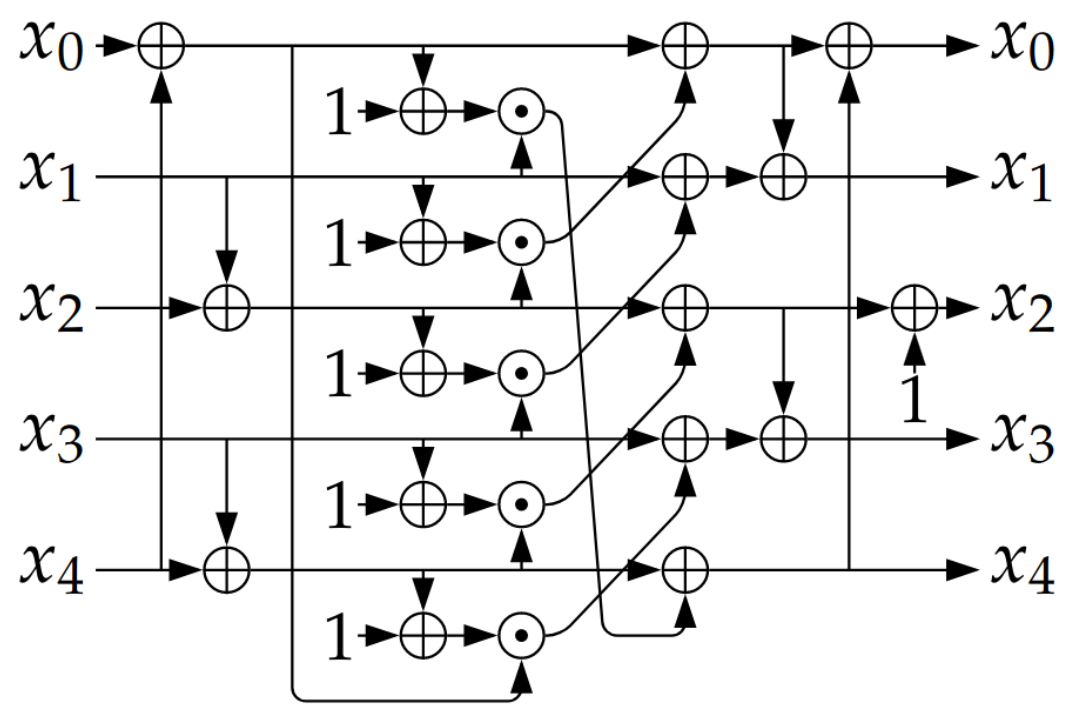
\includegraphics[width=0.5\linewidth]{img/to_harmonize/ascon.png}
    \caption{The 5-bits look-up table of ASCON. Figure extracted from \cite{JC:DEMS21}}
    \label{fig:ascon}
\end{figure}



This layout is a bit different from the others: the s-box takes five bits as input and outputs five bits. We denote $f_0, \dots, f_4$ the five functions of $\B^5 \mapsto \B$ that generate the 5 output bits $x_0, \dots, x_4$. Thus, we need to define five gadgets (one per function).

These functions, once analyzed by the algorithm, can be computed in one single bootstrapping each, but for different values of $p$ (respectively $p=17, 7, 7, 15, 11$ that are the smallest possible values). We could implement the gadgets $\Gamma_0, \dots, \Gamma_4$ (associated to $f_0, \dots, f_4$) with different values for $p_{in}$, but this would imply to introduce some encoding switchings before each round of hashing. To keep things simpler we generated only encodings with $p = 17$, making the implementation more straightforward as no encoding switching is required. For each subfunction $f_i$, five canonical $17$-encodings $(\Encoding_{i, 0}, \dots, \Encoding_{i, 4})$ of form $$\Encoding_{i, j} = \EncDefOne{d_{i,j}}$$ are computed. The results are displayed in the Table \ref{tab:encodings_ascon}. Note the zero values in some cases, they show that the variable is not used in the subfunction. 

The s-box layer is followed by a linear layer, where the bits of the states are shifted and combined with \texttt{XOR} operations. This can be trivially done with $p=2$. Finally, to prepare the next round, an encoding switching is performed to send back the ciphertexts on $17$-encodings. This is summed up in Figure \ref{fig:layout_spn}. Note that there is no encoding switching from non-linear layer to linear layer because the gadgets can directly outputs ciphertexts under $\Encoding_\oplus = \EncDefOne{1}$ with $p=2$.

\begin{figure}
    \centering
    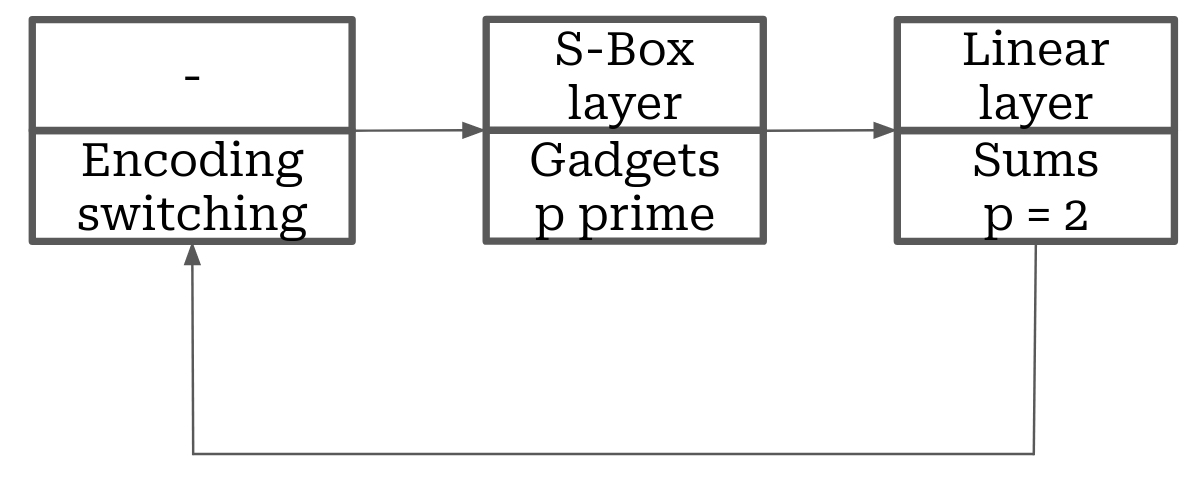
\includegraphics[width=0.5\linewidth]{img/to_harmonize/layout_spn.png}
    \caption{A common layout to evaluate cryptographic primitives. The upper part of the boxes represents what happens in the clear, while the lower part shows the encrypted operations. }
    \label{fig:layout_spn}
\end{figure}


To wrap up, we construct the five gadgets $\Gamma_i = \left ( (\Encoding_{i,0}, \dots,  \Encoding_{i, 4}), \Encoding_\oplus, 17, 2, f_i \right )$. They will carry the evaluation of the s-boxes and output ciphertexts encrypted under $\Encoding_\oplus$. Then, the linear layer is trivially evaluated with homomorphic sums. An encoding switching from $\Encoding_\oplus$ to $\Encoding_{i, j}$ allows to come back to non-linear operations.




\begin{table}[]
    \centering
    \begin{tabular}{|c|c|c|c|c|c|}
        \hline
       subfunction & $d_{i, 0}$ & $d_{i, 1}$ & $d_{i, 2}$ & $d_{i, 3}$ & $d_{i, 4}$\\
        \hline
        $f_0$  & $1$ & $2$ & $3$ & $7$ & $14$\\
        \hline
        $f_1$ & $1$ & $2$ & $2$ & $2$ & $4$\\
        \hline
        $f_2$ & $1$ & $2$ & $2$ & $4$ & $0$\\
        \hline
        $f_3$ & $1$ & $1$ & $5$ & $5$ & $3$\\
        \hline
        $f_4$ & $1$ & $2$ & $0$ & $4$ & $3$\\
        \hline
     \end{tabular}
    \caption{Parameters $d_{i, j}$ for Ascon, with $p=17$ for every subfunction.}
    \label{tab:encodings_ascon}
\end{table}


Using this solution, the s-box is evaluated in $92$ ms. Note that the 5 different PBS described in Table \ref{tab:encodings_ascon} have different norms of vector $\vec d$ so they may have a different set of parameters for each. We use the more restrictive one (i.e. the one with greater $\norm{\nu}$) for the 5. Estimating the timings of a full run of Ascon is not trivial because it depends a lot of the parameters. To give a rough idea, in hashing mode, 64 s-boxes are required per round, with 12 rounds recommended. The outputs of the s-boxes are in $\Z_2$ to allow the evaluation of the linear layer of Ascon. At the end of this linear layer, the encoding of each of the 320 bits of the state must be switched back to $\Z_{17}$ with a PBS. To do so, we use the same set of parameters as for the encoding switching in Step 3 of the Keccak evaluation in Section \ref{sec:keccak}.

This gives an estimation of $89$ seconds for one Ascon hash.


%\subsection{AES}
\label{sec:aes}

%\subsubsection{Reminders on AES and Choice of an Alternative Representation}

AES \cite{aes-original}, or Advanced Encryption Standard, stands as one of the most widely used and trusted encryption algorithms in the world of computer security. Its standardization occured in 2001 when it was adopted by NIST to replace the obsolete DES (Data Encryption Standard). Implementing this primitive in FHE is known as particularly tricky and only few attempts have been made \cite{C:GenHalSma12}, \cite{PKC:CorLepTib14}, \cite{trama-aes}.

A round of AES can be decomposed into 4 steps:
\begin{enumerate}
    \item \texttt{SubBytes}: a non-linear substitution step where each byte is replaced by another according to a lookup table. This step concentrates all the challenge for homomorphization, the other one being trivial with our framework.
    \item \texttt{ShiftRows}: a transposition step where the last three rows of the state are shifted cyclically a certain number of times. As our framework encrypts each bit in a distinct ciphertext, this step is for free.
    \item \texttt{MixColumns}: a linear mixing operation which operates on the columns of the state, combining the four bytes in each column. This step can be implemented using only \texttt{XOR} operations and bit-shiftings. The former are trivial with our framework using $p=2$ and the latter are for free as the ones in the previous step.
    \item \texttt{AddRoundKey}: each byte of the state is combined with a byte of the key from the key schedule using a \texttt{XOR}. Still using $p=2$, this can be carried out easily. 
\end{enumerate}


 The s-box of \texttt{SubBytes} takes 8 bits in input and yields 8 bits of output. It is defined by two substeps: an inversion in $GF(2^8)$ followed by an affine transformation. While the latter is trivial to compute with TFHE, the former is much trickier and thus we did not take advantage of this representation. Using our framework, the obvious-looking solution is to split the full s-box $\B^8 \mapsto \B^8$ into 8 subfunctions $f_0, \dots, f_7: \B^8 \mapsto \B$. We could then give them to the search algorithm of Section \ref{sec:search}. If this would work, we could evaluate the Rjindael s-box in 8 PBS. Unfortunately, the algorithm does not converge for values of $p$ ``reasonable'', that is to say less than 7 bits. 


We thus need to leverage an alternative representation of the s-box. A well known efficient Boolean representation of the AES s-box is given in \cite{boyar}. In this work, authors applied logic minimization techniques to produce an optimized Boolean circuit (in terms of number of gates) of the s-box splitted in 3 phases:

\begin{enumerate}
    \item A purely linear layer mapping the 8 input bits onto 22 bits.
    \item A middle non-linear layer, represented by a circuit with exclusively \texttt{AND} and \texttt{XOR} logic gates, mapping the previous 22 bits onto 18 bits.
    \item A final purely linear layer mapping the 18 bits on the 8 output bits of the s-box.
\end{enumerate}


To design our implementation of AES, we will use the strategy we introduced for Keccak (Section \ref{sec:keccak}) and ASCON (Section \ref{sec:ascon}) and that is illustrated on Figure \ref{fig:layout_spn}. The steps \texttt{ShiftRows}, \texttt{MixColumns}, \texttt{AddRoundKeys} only involves \texttt{XOR} operators, so we will carry them out with $p=2$. Same things with the steps 1. and 3. of the circuit of \texttt{SubBytes} of \cite{boyar}. The only part remaining is the Step 2. of the \texttt{SubBytes}, that is a non-linear circuit. We evaluate this circuit using gadgets and the approach introduced in Section \ref{sec:graphs}. A layer of encoding switching allows to link both parts.

 In particular, \texttt{MixColumns} can be reduced to a serie of \texttt{XOR} (in our implementation, we use the circuit designed in \cite{mixcol}). 

In the following, we focus on the implementation of the non-linear layer using the approach by graphs of Section \ref{sec:graphs}.


\subsubsection{Homomorphization of the S-box}


We start from the circuit representation given in the work of \cite{boyar}. This set of instructions is compiled into a circuit $\mathcal{A}$, compliant with the definitions introduced in Section \ref{sec:graph_definition}.


Each of the $18$ outputs $(z_0, \dots, z_{17})$ are isolated from each other and the circuits $(\mathcal{A}_0, \dots, \mathcal{A}_{17})$ generating them are separated. Of course, some intermediary values are used in several circuits, but for now we ignore this and we considerate the $18$ problems as independent from each other. 

Then, for each circuit $\mathcal{A}_i$, we run the algorithm explained in Section \ref{sec:graphs} to produce an efficient graph. We merge all those graphs and run everything for a total of 36 PBS to evaluate the full circuit $\mathcal{A}$, with a global $p = 11$. This allows a relatively quick bootstrapping.

Recall that the \texttt{SubBytes} step is made of 16 s-boxes. So, we can derive that one execution of the \texttt{SubBytes} step takes $16 \times 36 = 576$ PBS. 

The outputs of this step would be encoded with $p=2$, allowing the \texttt{XOR} operations of the following steps to be performed efficiently. We also need to take into account the encoding switching to come back to $p=11$ before each \texttt{SubBytes}. It costs one PBS per bit, so $128$ PBS. Finally, this gives a total of $704$ PBS per round. For \texttt{AES-128}, which takes 10 rounds, we estimate a full run to $7040$ PBS.

\subsubsection{Performances}

In terms of performances, with a set of parameters ensuring a security level of $\lambda=128$ bits and an error probability $\epsilon=2^{-40}$, a PBS takes $17$ ms on our hardware. The total runtime of the whole implementation on one thread is $135$ s. We note that the $16$ evaluations of s-boxes in \texttt{SubBytes} can be parallelized, as well as each of the $128$ encoding switchings before \texttt{SubBytes}. Moreover, within each s-box, we can locally apply our strategy of parallelization introduced in Section \ref{sec:parallelization}.


We compare favorably to previous works of \cite{C:GenHalSma12} and \cite{PKC:CorLepTib14}, who report timings of respectively 18~minutes and 5~minutes for a full AES, Once again, authors do not mention the value of $\epsilon$. The more recent work of \cite{trama-aes}, also proposes an implementation of \texttt{AES-128} using a completely different technique called the \emph{tree-bootstrapping}. On a similar experimental setup, but with a failure probability $\epsilon=2^{-23}$, they claim an execution in $270$~s on one thread. We ran again our code with an other set of parameters tailored for the same $\epsilon$ and obtained a full run in $103$~s.  Note that in our implementation, we used the mode restrictive set of parameters $\texttt{PBS}_{(11, 4)}$ for every bootstrapping (even the ones that should be performed with $\texttt{PBS}_{(2, 1}$. We also derived the theoretical timing that could have been achieved if we had implemented this with two server keys (one for each set of parameters). This theoretical timing should be of $105$ s with $\epsilon=2^{-40}$, we added it in Table \ref{tab:concrete_perfs}.


\subsection{Summary of Applications}
\label{sec:tables_perfs}


We summarize hereafter the parameters and performances of our implementations of cryptographic primitives. Table~\ref{tab:parameters} gives an overview of the TFHE parameters used for each value of $p$ in these examples. They all meet the required level of security of $2^{128}$ and the error probability $\epsilon=2^{-40}$. It also shows the associated $p$ and the norm of $\vec d$, denoted by $\mathcal{N}_{\vec d}$ (that corresponds to $\mathcal{N}_{\vec d} = \lceil \log_2(\customnorm{\vec d}) \rceil$) that are the input of the parameter selection algorithm. To allow the comparison with the strategy of gate bootstrapping, we also included the set of parameters hardcoded in \texttt{tfhe-rs} to evaluate boolean operators. Table \ref{tab:complexity_primitives} shows the complexity of the cryptographic primitives expressed in PBS with our framework. It can be compared with Table \ref{tab:gates}, that illustrates the number of PBS required with the naive strategy of gate bootstrapping. Finally, Table \ref{tab:concrete_perfs} shows the concrete performance achieved by our implementations on our machine, as well as the comparison with other works and with the gate bootstrapping. For more information about an implementation or a comparison, the reader is referred to the related section.

\newcommand{\PBS}{\mathsf{PBS}}

\begin{table}
    \centering
    \small % Adjust font size if necessary
    \begin{tabular}{|l|c||c|c|c|c|c|c|c|c|c||c|}
            \hline
        \multicolumn{2}{|c||}{\textbf{Identification}} & \multicolumn{9}{c||}{\textbf{TFHE parameters}} & \textbf{Timings} \\
        \hline
        Ref. & Sections & $n$ & $k$ & $N$ & $\sigma_{\texttt{\LWE}}$ & $\sigma_{\texttt{\GLWE}}$ & $B_g$ & $\ell_g$ & $B_{KS}$ & $\ell_{KS}$ & PBS\\
        \hline
        \hline
            \texttt{$\PBS_{gate}$} & Table \ref{tab:gates} & 722 & 2 & 512 & $2^{16.2}$ & $2^{7.8}$ & $2^6$ & 3 & $2^3$ & 4 & 10 ms\\
           \hline
          \hline
        \texttt{$\PBS_{(9, 2)}$} & \ref{sec:simon}, \ref{sec:trivium} & 684 & 3 & 512 & $2^{16}$ & $2^{2}$& $2^{10}$ & 2 & $2^3$ & 4 & 9.5 ms\\
           \hline
       
        \texttt{$\PBS_{(3, 2)}$} & \ref{sec:keccak} & 676 & 5 & 256 & $2^{22}$ & $2^{7}$& $2^{18}$ & 1 & $2^4$ & 3 & 5.25 ms \\
          \hline
    
        \texttt{$\PBS_{(2, 1)}$} & \ref{sec:keccak}, \ref{sec:ascon} & 676 & 5 & 256 & $2^{22}$ & $2^{7}$& $2^{18}$ & 1 & $2^4$ & 3 & 5.25 ms \\
         \hline
        
        \texttt{$\PBS_{(17, 5)}$} & \ref{sec:ascon} & 740 & 2 & 1024 & $2^{13}$ & $2^{2}$& $2^7$ & 3 & $2^5$ & 3 & 18 ms\\
         \hline
        
        \texttt{$\PBS_{(11, 4)}$} & \ref{sec:aes} & 708 & 3 & 512 & $2^{15}$ & $2^{2}$& $2^6$ & 4 & $2^2$ & 7 & 17 ms  \\
            \hline
       \end{tabular}

    \medskip 
    
    \caption{Sets of TFHE parameters for each PBS used in our implementations, with the constraints used to generate the sets, and the performances. Each setting is referenced as \texttt{$\PBS_{(p, \mathcal{N}_d)}$} with $\mathcal{N}_d = \lceil \log_2(\customnorm{d})\rceil$. All this parameters ensure a level of security $\lambda=128$ bits and a failure probability of bootstrapping of $\epsilon=2^{-40}$. $q$ is always fixed to $2^{32}$. \texttt{$\PBS_{gate}$} refers to the naive case of the gate bootstrapping implemented in \cite{tfhe-rs} and is used to estimate the timings of the naive strategy in Table \ref{tab:concrete_perfs}.}
    \label{tab:parameters}
\end{table}



\begin{table}
    \centering
    \begin{tabular}{|c|c|c|}
        \hline
        \textbf{Section} & \textbf{Primitive} & \textbf{Complexity in PBS}  \\
        \hline
        \multirow{2}{*}{\ref{sec:simon}} & One round of SIMON-128 & 64 \texttt{$\PBS_{(9, 2)}$}\\
        \cline{2-3}
        & One full run of SIMON-128 & 4352 \texttt{$\PBS_{(9, 2)}$}\\
        \hline
        \multirow{2}{*}{\ref{sec:trivium}} & One round of Trivium & 3 \texttt{$\PBS_{(9, 2)}$}\\
        \cline{2-3}
        & ~One warm-up phase of Trivium $(*)$~ & 3456 \texttt{$\PBS_{(9, 2)}$}\\
        \hline
        \multirow{2}{*}{\ref{sec:keccak}} & One round of Keccak & 1600 \texttt{$\PBS_{(3, 2)}$} $+$ 1600 \texttt{$\PBS_{(2, 1)}$}\\
        \cline{2-3}
        & A full Keccak permutation $(*)$ & ~38400 \texttt{$\PBS_{(3, 2)}$} $+$ 38400 \texttt{$\PBS_{(2, 1)}$} ~\\
        \hline
      \multirow{2}{*}{ \ref{sec:ascon}} & One evaluation of Ascon's s-box & 5 \texttt{$\PBS_{(17, 5)}$}\\
      \cline{2-3}
      & One full Ascon hashing run $(*)$ & 3840 \texttt{$\PBS_{(17, 5)} + 3840 \PBS_{(2, 1)}$}\\
        \hline
        \multirow{2}{*}{\ref{sec:aes}} & One evaluation of the AES s-box & 36 \texttt{$\PBS_{(11, 4)}$}\\
        \cline{2-3}
        & A full run of \texttt{AES-128}  & 5760 \texttt{$\PBS_{(11, 4)}$} + 1280 \texttt{$\PBS_{(2, 1)}$}\\
        \hline
    \end{tabular}
    \medskip
    \caption{Complexity of the different primitives we implemented with respect to the PBS of Table~\ref{tab:parameters}. The primitives indicated by a $(*)$ are estimations while the others have been fully implemented.}
    \label{tab:complexity_primitives}
\end{table}



\begin{table}
    \centering
    \begin{tabular}{|c|c|c|}
        \hline
        \textbf{Section} & \textbf{Primitive} & \textbf{Number of logic gates}  \\
        \hline
        \multirow{2}{*}{\ref{sec:simon}} & One round of SIMON-128 & 256\\
        \cline{2-3}
        & One full run of SIMON-128 & 17408\\
        \hline
        \multirow{2}{*}{\ref{sec:trivium}} & One round of Trivium & 13\\
        \cline{2-3}
        & ~One warm-up phase of Trivium $(*)$~ & 14976\\
        \hline
        \multirow{2}{*}{\ref{sec:keccak}} & One round of Keccak & 7687\\
        \cline{2-3}
        & A full Keccak permutation $(*)$ & 184488\\
        \hline
      \multirow{2}{*}{ \ref{sec:ascon}} & One evaluation of Ascon's s-box & 16\\
      \cline{2-3}
      & One full Ascon hashing run $(*)$ & 19968\\
        \hline
        \multirow{2}{*}{\ref{sec:aes}} & One evaluation of the AES s-box & 115 (\cite{boyar})\\
        \cline{2-3}
        & A full run of \texttt{AES-128}  & 23360 (\cite{boyar}, \cite{mixcol})\\
        \hline
    \end{tabular}
    \medskip
    \caption{Number of logic gates in the circuit of each primitive. This shows the heavy cost of the naive method of performing one bootstrapping per gate (except the \texttt{NOT} ones).}
    \label{tab:gates}
\end{table}


\begin{table}
    \centering
    \scalebox{0.9}{
    \begin{tabular}{|c|c|c|}
    \hline
       \textbf{Primitive} & \textbf{Section or Other work} & \textbf{Performances} \\
    \hline
    \hline
        \multirow{3}{*}{One full run of SIMON} & Gate Bootstrapping & 174 s\\
        \cline{2-3}
        & \cite{cryptoeprint:2023/480} $\dagger$ & 128 s\\
        \cline{2-3}
         & Our work (Section \ref{sec:simon}) & 10 s \\
         \hline
         \hline
         \multirow{3}{*}{One warm-up phase of Trivium (*)} & Gate Bootstrapping & 1498 s\\
         \cline{2-3}
         & ~\cite{DBLP:conf/wahc/BalenboisOS23} (estimation on our machine)~ & 53 s\\
        \cline{2-3}
         & Our work (Section \ref{sec:trivium}) & 32.8 s\\
         \hline
         \hline
        \multirow{2}{*}{One Full Keccak permutation $(*)$} & Gate Bootstrapping & 30.7 min\\
        \cline{2-3}
        & Our work (Section \ref{sec:keccak}) & 8.8 min\\
        \hline
        \hline
        \multirow{2}{*}{One Ascon hashing $(*)$} & Gate Bootstrapping & 200s \\
        \cline{2-3}
        & Our work (Section \ref{sec:ascon}) & 92 s \\
        \hline
        \hline
        \multirow{4}{*}{\begin{tabular}{c}
            One full evaluation of AES-128   \\
            ($\epsilon=2^{-23}$) on one thread \\
        \end{tabular}} & \cite{C:GenHalSma12} $\dagger$ & 18 min\\
        \cline{2-3}
        & \cite{PKC:CorLepTib14} $\dagger$ & 5 min\\
        \cline{2-3}
        & \cite{trama-aes} & 270 s\\
        \cline{2-3}
        & Our work (Section \ref{sec:aes}) & 103 s\\
    \hline
        \multirow{3}{*}{\begin{tabular}{c}
            One full evaluation of AES-128   \\
            ($\epsilon=2^{-40}$) on one thread \\
        \end{tabular}} & Gate Bootstrapping & 234 s \\
        \cline{2-3}
        & Our work (Real implementation) & 135 s\\
        \cline{2-3}
        & Our work (Theoretical timing with two keys) & 105 s\\
    \hline
    \end{tabular}}
    
    \medskip 
    
    \caption{Timings of evaluation of full primitives, and comparison with previous works when they exist. Like on Table \ref{tab:complexity_primitives}, a star $(*)$ is added in the cells if our timing is not obtained from a full implementation but estimated from an implemented building block. Also, the security level of each implementation is $\lambda=128$ and the default error probability is $\epsilon=2^{-40}$. The concurrent works that do not indicates their $\epsilon$ are marked with $\dagger$. }
    \label{tab:concrete_perfs}
\end{table}

%\section{Conclusion}

In this chapter, we presented a first application of our technique of using an odd plaintext modulus: by embedding $\ell$ bits into a prime field, it becomes possible to unlock the full potential of homomorphic addition and ``pack'' several bits into a ciphertext. We can then retrieve the result of any Boolean function $f:\B^\ell \mapsto \B$ by a unique bootstrapping. This approach scales much better than the conventional technique of using a \gls{LUT} of size $2^\ell$.

We ended this chapter by presenting an homomorphic implementation of the \gls{AES} scheme. Implementing the circuit of the S-box using our technique was by far the most challenging part of this design. This is not very surprising: this component has been designed to prevent cryptanalysis,  which indirectly makes the circuit representation of this function unsuitable for this kind of Boolean-oriented approaches.

An interesting axis of improvement would be to use an \textit{arithmetic} representation of the values, so the S-box would simply be evaluated as a \gls{LUT}. But by fully committing to arithmetic representation, the linear part of the scheme (so the \ShiftRows, \MixColumns and \AddRoundKey steps) becomes the new bottleneck, as we could not leverage the additive homomorphism of \gls{TFHE} to evaluate XOR operations anymore. In the next chapter, we elaborate further on these ideas and construct a more efficient version of homomorphic \gls{AES} by combining both Boolean and arithmetic representations. 





\chapter[Acceleration of Homomorphic Boolean Functions]{A first application: Accelerating Boolean circuits evaluation with $p$-encodings}
\label{chap:p_encodings}

\TODO{repasser sur l'intro}

%% !TeX_ROOT=../../thesis.tex


\gls{TFHE} being the most efficient scheme to handle data of small precision, it is a natural choice when it comes to evaluate homomorphically Boolean circuits. However, performances of the existing frameworks are still limited. 

The most straightforward method, already introduced in the original \gls{TFHE} paper \cite{JC:CGGI20} under the name \emph{gate bootstrapping}, consists in running one bootstrapping for each bivariate Boolean gate of the circuit. As a consequence, the conversion of the original Boolean circuit in a homomorphic circuit handling encrypted bits is straightforward, moreover the noise growth is contained thanks to the systematic use of bootstrapping. However, this approach is very expensive due to the high numbers of bootstrappings and makes it quite suboptimal for large circuits.


In this chapter, we introduce a new framework to homomorphically evaluate Boolean functions on encrypted data efficiently, i.e. by reducing the amount of necessary bootstrappings. Our approach introduces an \emph{intermediate homomorphic layer} which encodes the bits (elements of $\Z_2$) on a small ring $\Z_p$ before encrypting them. This allows us to evaluate Boolean functions with one cheap homomorphic sum followed by one bootstrapping. After formalizing the underlying concept of $p$-\emph{encoding} and explaining our evaluation strategy, we investigate the issue of finding valid sets of encodings for a Boolean function. We characterize this problem and provide an exact constructive algorithm to solve it. We further provide a sieving heuristic finding solutions more efficiently but at the cost of loosing optimally. Since our method is only efficient for Boolean functions with limited number of inputs, we also propose a heuristic to decompose any Boolean circuit into Boolean functions which are efficiently evaluable using our approach. Finally, we apply our technique to various cryptographic primitives, namely the SIMON block cipher, the Trivium stream cipher, the Keccak permutation, the Ascon S-box and the \gls{AES} S-box. Compared to previous works implementing the same primitives (for SIMON, Trivium and \gls{AES}) our implementations achieve significant speedups.

After some technical preliminaries on Boolean circuits (Section \ref{sec:p_encodings_preliminaries_boolean}), we introduce a new concept of \emph{intermediate homomorphic layer} and explain how bits are encoded  in Section \ref{sec:p_encodings_homorphic_layer} and the algorithms to construct it in Sections \ref{sec:p_encodings_search} and \ref{sec:p_encodings_graphs}. Finally, we describe some implementation works in Section \ref{sec:p_encodings_TFHE_adaptation} and our experimental results in Section \ref{sec:p_encodings_implementations}.











\section{Preliminaries on Boolean Functions and Boolean Circuits}
\label{sec:p_encodings_preliminaries_boolean}


A Boolean function has the form $f: \B^\ell \longrightarrow \B$, with $\ell$ being called the \emph{arity} of the function. 

\begin{definition}
    
The Algebraic Normal Form (ANF) of a Boolean function $f: \{0,1\}^\ell \mapsto \{0,1\}$ is a polynomial expression in which each term corresponds to a specific input combination of $n$ variables. The ANF is defined as follows: \[f(x_1, x_2, \ldots, x_l) = a_0 \oplus a_1x_1 \oplus a_2x_2 \oplus \ldots \oplus a_{2^n-1}x_1x_2\ldots x_l\] \begin{align*}
\text{where: }a_0, a_1, a_2, \ldots, a_{2^\ell-1} & \in \{0,1\} \quad \text{are the Boolean coefficients and} \\
x_1, x_2, \ldots, x_\ell & \quad \text{are called the Boolean variables}
\end{align*}
\end{definition}

This result means that any Boolean function can be evaluated by the means of \texttt{AND} and \texttt{XOR} operations. In the following, we will focus on the implementation of Boolean circuits composed of these operations exclusively.


A Boolean function can be represented by its \emph{truth table}, which is simply a table gathering all the possible inputs and the corresponding result of the application by the function. It can also be represented with a Boolean formula. A third representation is the \emph{Boolean circuit}:

\begin{definition}
    A Boolean circuit associated to the Boolean function $f$ is a finite Directed Acyclic Graph whose edges are \emph{wires} and vertices are \emph{Boolean gates} representing Boolean operations. We consider \texttt{AND} gates and \texttt{XOR} gates, of fan-in 2 and fan-out 1. We also consider copy gates, of fan-in 1 and fan-out $>1$, that outputs several copies of its input. A circuit is further formally composed of input gates of fan-in 0 and fan-out 1, and output gates of fan-in 1 and fan-out 0.
    
    Evaluating a $\ell$-input $m$-output circuit consists in writing an input $\vec{x} \in \B^\ell$ in the input gates, processing the gates from input gates to output gates, then reading the outputs from the output gates.

\end{definition}


This notion of Boolean circuit will be particularly useful in Section \ref{sec:p_encodings_graphs}.


\section{Boolean Encoding over $\Z_p$ and Homomorphic Evaluation Strategy Between $\B$ and $\Z_p$}
\label{sec:p_encodings_homorphic_layer}



We propose a construction in which we embed Boolean values in $\Z_p$ for well-chosen values of $p$, forming an ``intermediate homomorphic layer'' between $\B$ (the plaintext space of bits) and $\Z_q$ (the ciphertext space). In the following, we explain how we define such a layer, and we describe our new strategy to evaluate Boolean functions in a more efficient way without considering the circuit representation of the function. Note that we generalize this construction to arithmetic spaces in Chapter \ref{chap:hyppogriph}.


\subsection{Encoding of $\B$ over $\Z_p$}

To represent Boolean values over $\Z_p$, we use a mapping function that we call a \emph{$p$-encoding}:

\begin{definition}[$p$-encoding]
    A \emph{$p$-encoding} is a function $\Encoding: \B \mapsto 2^{\Z_p}$ that maps the Boolean space to a subset of the discretized torus. A $p$-encoding is \emph{valid} if and only if:
    \begin{equation}
        \begin{cases}
            \Encoding(0) \cap \Encoding(1) = \emptyset~\text{ and}\\
            \text{if $p$ is even:} ~\forall \:x \in \mathbb Z_p, \forall \:b \in \B: x \in \Encoding(b) \iff \left [ x + \frac p 2 \right ]_p \notin \Encoding(b)
        \end{cases}
    \label{def:validity}
    \end{equation}
    We call this last property \emph{relaxed negacyclicity}.
    \label{def:encoding}
\end{definition}



\begin{figure}[ht]
	\centering
	\begin{minipage}{0.45\textwidth}
		\centering
		\begin{tikzpicture}[scale=0.8]
			\drawSingleRingGreenRed{15}{small}{true}{true}{9, 10}{0, 8, 11, 12, 14}
		\end{tikzpicture}
		\caption*{Example with $p=15$}
	\end{minipage}
	\hfill
	\begin{minipage}{0.45\textwidth}
		\centering
		\begin{tikzpicture}[scale=0.8]
			\drawSingleRingGreenRed{16}{small}{true}{true}{8, 12, 13}{0, 4, 9, 11}
		\end{tikzpicture}
		\caption*{Example with $p=16$}
	\end{minipage}
	
	\caption{Representation of two valid $p$-encodings. The green part represents $\Encoding(1)$,  and the red part $\Encoding(0)$. Note that even if $p$ is even on the right-hand figure, the relaxed negacyclity is still respected.}
\end{figure}


In our approach when we need to encrypt a bit, we apply a $p$-encoding to embed it in $\Z_p$, then we encrypt the result using the classical setup of TFHE.  When new values are freshly encrypted or produced by a PBS, only one element of $ \Z_p$ is chosen for each bit. We call such an encoding a canonical $p$-encoding:

\begin{definition}[Canonical Encoding]
    A $p$-encoding $\Encoding$ is said \emph{canonical} if and only if it is valid and $\left| \Encoding(0) \right| = \left| \Encoding(1) \right| = 1$
    \label{def:canonical}
\end{definition}


Let $c$ be a ciphertext encoding a bit $b$ under a $p$-encoding $\Encoding$, where $\Encoding$ is an arbitrary valid encoding: its associated subsets can be any subset of $\Z_p$ as long as the validity requirements of (\ref{def:validity}) are fulfilled. One can transform the ciphertext $c$ into another ciphertext $c'$ encoded under any \emph{canonical} $p$-encoding, possibly under a different $p$, by simply performing a PBS.


\begin{property} [Reduction to a canonical encoding]
    \label{prop:cast_valid_to_canonical}
    Let $\Encoding$ be a valid $p$-encoding and $\Encoding'$ a canonical $p'$-encoding. We denote $\alpha' = \Encoding'(0)$ and $\beta' = \Encoding'(1)$. Let $c$ be a ciphertext encrypting a bit $b$ under $\Encoding$. Then, one can produce a ciphertext $c'$ encrypting the same bit $b$ under $\Encoding'$ by applying a PBS on $c$. This PBS performs the function :
    \[
        \begin{aligned}
            \texttt{Cast}_{\Encoding \mapsto \Encoding'}~:~& \Z_p \mapsto \Z_{p'}\\
            & x \mapsto \begin{cases}
                            \alpha' & \text{ if } x \in \Encoding(0)\\
                            \beta' & \text{ if } x \in \Encoding(1)\\
                            \bot & \text{ otherwise.}
                        \end{cases}
        \end{aligned}
    \]
    Here, $\bot$ simply denotes a placeholder value for a state that cannot be reached.
\end{property}



Our goal is to represent the Boolean function we want to evaluate with a sum of $p$-encodings (we define what we mean by ``sum of $p$-encoding'' in Section \ref{sec:p_encodings_new_strategy}).  When sums are carried out on ciphertexts (and so homomorphically on the underlying $p$-encodings), the sets $\Encoding(0)$ and $\Encoding(1)$ of the $p$-encodings may move, grow, shrink, but they should never overlap as it would result in a loss of information. As we removed the need for a bit of padding, we do not need to track a potential overflow of data (informally we say that ciphertexts are free to ``loop around the torus''). After the sum, the encoding of the result can be reset to a canonical one with a PBS to allow further computation. Or, if the homomorphic computation is over, the result can be recovered by decrypting the ciphertext and checking in which partition the decrypted value lies.


The next subsection explains in further details the process of evaluating Boolean functions on with $p$-encodings.



\subsection{A New Strategy for Homomorphic Boolean Evaluation}
\label{sec:p_encodings_new_strategy}



In the following, we consider two Boolean variables $x$ and $y$ and their two respective encodings over $\Z_p$: 
\begin{equation}
\Encoding_x = 
\EncDef{\{\alpha_i\}_{0 \le i \le l_0}}{\{\beta_i\}_{0 \le i \le l_1}} \text{ and } \Encoding_y = \EncDef{\{\alpha'_i\}_{0 \le i \le l'_0}}{\{\beta'_i\}_{0 \le i \le l'_1}}
\label{eq:encoding_definition}
\end{equation}


Let $f$ be a bivariate Boolean function and let us construct two sets $\mathcal{P}_0$ and $\mathcal{P}_1$ such that:
\begin{equation}
    \mathcal{P}_b = \{[\gamma + \delta]_p \mid (\gamma, \delta) \in \Encoding_x(b_x) \times \Encoding_y(b_y) \text{ and } f(b_x, b_y) = b \text{ with } (b_x, b_y) \in \B^2\}~\forall~b \in \B.
    \label{def:sets_p}
\end{equation}

We say that the sum of $p$-encodings $\Encoding_x + \Encoding_y$ is \emph{suitable for the evaluation of $f$} if and only if $\mathcal{P}_0 \cap \mathcal{P}_1 = \emptyset$. The definition can be generalized to any number of arguments $\ell$ for $f$. For a given $f$, finding such correct encodings is not trivial. We elaborate further on this point in Section \ref{sec:search}. 

If $\Encoding_x$ and $\Encoding_y$ are suitable for $f$, then one can use the computed sets $\mathcal{P}_0$ and $\mathcal{P}_1$ to construct a new $p$-encoding \[\Encoding_z = \EncDef{\mathcal{P}_0}{\mathcal{P}_1}\] that encodes the bit $f(x, y)$. As $\Encoding_z$ is valid, then the clear value of the bit can be recovered by decryption, or further computations can be performed without the need of a bootstrapping. 


\begin{definition}[Application of a function to a vector of encodings]
    Let $f:\B^\ell \mapsto \B$ be a Boolean function and let $\vec \Encoding = (\Encoding_1, \dots, \Encoding_l)$ be a vector of $p$-encodings. We define $f(\vec \Encoding)$ by:
    \[f(\vec \Encoding) = \EncDef{\mathcal{P}_0}{\mathcal{P}_1}\]
    with: 
    \[\mathcal{P}_b = \left \{ \left [ \sum_{i=1}^{l} \gamma_i \right ]_p \mid (\gamma_1, \dots, \gamma_l) \in \prod_{i=1}^\ell \Encoding_i(b_i) \text{ and } f(b_1, \dots, b_l) = b \right \} \forall b \in \B\]

$f(\vec \Encoding)$ always exists, but is valid only if it respects the constraints of Definition \ref{def:validity}.
\end{definition}


Let us illustrate the latter definition on two toy example. We consider the two Boolean operators $\&$ and $\oplus$. The $p$-encoding resulting of the function $f: (x, y) \mapsto x ~\&~ y$ is: 

\begin{equation}
\Encoding_\& = \begin{cases}
0 \mapsto \{\alpha_i + \alpha'_j\}_{\substack{0\le i \le l_0 \\ 0 \le j \le l_0'}} \cup \{\alpha_i + \beta'_j\}_{\substack{0 \le i \le l_0 \\ 0 \le j \le l'_1}} \cup \{\alpha'_i + \beta_j\}_{\substack{0 \le i \le l'_0 \\ 0 \le j \le l_1}}\\
1 \mapsto \{\beta_i + \beta'_j\}_{\substack{0\le i \le l_1 \\ 0 \le j \le l_1'}}
\end{cases}
\label{eq:encoding_and}
\end{equation}
and the $p$-encoding resulting of the operation $f: (x, y) \mapsto x \oplus y$ is:

\begin{equation}
\Encoding_\oplus = \begin{cases}
0 \mapsto \{\alpha_i + \alpha'_j\}_{\substack{0\le i \le l_0 \\ 0 \le j \le l_0'}} \cup \{\beta_i + \beta'_j\}_{\substack{0 \le i \le l'_0 \\ 0 \le j \le l'_1}}\\
1 \mapsto \{\alpha_i + \beta'_j\}_{\substack{0\le i \le l_0 \\ 0 \le j \le l_1'}} \cup \{\alpha'_i + \beta_j\}_{\substack{0\le i \le l_0' \\ 0 \le j \le l_1}} \\
\end{cases}
\label{eq:encoding_xor}
\end{equation}
%
Figure \ref{fig:operations} further illustrates this construction for these two operations.

\begin{figure}
	\centering
	\begin{tikzpicture}
		\drawSingleRingGreenRedBox{15}{small}{true}{6}{9}{0}{0}{0.5}{}
		\node at (2.5, 0) {\Huge $\&$};
		\drawSingleRingGreenRedBox{15}{small}{true}{4}{5}{10}{0}{0.5}{}
		\node at (7.5, 0) {\Huge $=$};
		\drawSingleRingGreenRedBox{15}{small}{true}{10}{11, 13, 14}{20}{0}{0.5}{}
		
		\drawSingleRingGreenRedBox{15}{small}{true}{6}{9}{0}{-10}{0.5}{}
		\node at (2.5, -5) {\Huge $\oplus$};
		\drawSingleRingGreenRedBox{15}{small}{true}{4}{5}{10}{-10}{0.5}{}
		\node at (7.5, -5) {\Huge $=$};
		\drawSingleRingGreenRedBox{15}{small}{true}{10}{11, 13, 14}{20}{-10}{0.5}{}
	\end{tikzpicture}
	\caption{Starting from two canonical encodings, we produce two new $p$-encodings corresponding to the results of the $\&$ and the $\oplus$ operations.}
	\label{fig:operations}
\end{figure}


To wrap up, here is our proposed framework to evaluate a Boolean function $f: \B^\ell \mapsto \B$ given a vector of suitable $p$-encodings $\Encoding = (\Encoding_1, \dots, \Encoding_l)$:

\begin{enumerate}
\item Encrypt each input $b_i$ with some canonical $p$-encoding $\Encoding_i$ into a ciphertext $c_i$ such that $\Encoding_{sum} = f(\Encoding_1, \dots, \Encoding_\ell)$ is a valid encoding.
\item For a Boolean function $f$ to be evaluated on $b_1, \dots, b_\ell$, compute homomorphically the sum of the ciphertexts $c = c_1 + \dots + c_\ell$. This yields an encryption of $b = f(b_1, \dots, b_\ell)$, encoded with a valid $p$-encoding $\Encoding_{sum} = f(\Encoding_1, \dots, \Encoding_\ell)$.
\item \begin{enumerate}
    \item If the result is directly required by the client, $c$ is returned as ciphertext which can be decrypted to get the result in $\Z_p$ and associated to the right Boolean value.
    \item If the result is reused in further homomorphic computations, a PBS calculating $\texttt{Cast}_{\Encoding_{sum} \mapsto \Encoding_{new}}$ on the result is computed (like introduced in Property \ref{prop:cast_valid_to_canonical}), with $\Encoding_{new}$ a new canonical $p$-encoding. The resulting value can then be used as an input for a next Boolean function.
    \end{enumerate}
\end{enumerate}

Let us formalize this process by defining the notion of \textit{gadget associated to a Boolean function $f$} :
\begin{definition}[Gadget]
    Let $f$ be a Boolean function of arity $\ell$.
    A gadget associated to $f$ is an homomorphic operator defined by a tuple $\Gamma = \left ( \vec{\Encoding_{in}} = (\Encoding_{in}^{(1)}, \dots, \Encoding_{in}^{(\ell)}), \Encoding_{out}, p_{in}, p_{out} \right )$ such that:
    \begin{itemize}
        \item All the elements of $\vec{\Encoding_{in}}$ are $p_{in}$-encodings, and $\Encoding_{out}$ is a canonical $p_{out}$-encoding.
        \item The encoding $\Encoding_{sum} = f(\Encoding_{in}^{(1)}, \dots, \Encoding_{in}^{(\ell)})$ is a valid encoding.
    \end{itemize}
Applying a gadget to ciphertexts  $c1, \dots, c_\ell$, that encrypt the bits $b_1, \dots, b_\ell$, produces a new ciphertext $c'$ encrypting the bit $f(b_1, \dots, b_\ell)$ under the $p_{out}$-encoding $\Encoding_{out}$. To do so, we perform the following algorithm:
\begin{itemize}
    \item Constructing an intermediate ciphertext $c_{inter} = \sum_{i=1}^{\ell} c_i$ using the homomorphic sum of TFHE. This ciphertext encrypts $f(b_1, \dots, b_\ell)$ under the $p_{in}$-encoding $f(\Encoding_1, \dots, \Encoding_\ell)$.
    \item Reducing the encoding of $c_{inter}$ from $\Encoding_{inter}$ to $\Encoding_{out}$ by applying a PBS on $c_{inter}$ performing the function $\texttt{Cast}_{\Encoding_{inter} \mapsto \Encoding_{out}}$. This produces the expected result $c'$.
    \end{itemize}
\label{def:gadget}
\end{definition}


The advantage of this construction is that only one PBS is performed to apply the function. Moreover, depending on the function, the input size of the PBS lookup table might be much smaller than the arity of the function. Gadgets can be seen as a way to compress several Boolean operators into a single evaluation of univariate look-up table.
Of course, for a given $p_{in}$ and a given $f$, such a gadget may not exist. In such a case, two solutions can be considered:
\begin{itemize}
    \item Increasing the value of $p_{in}$ (e.g.  taking $p_{in} \ge 2^\ell$ always works, but is very inefficient).
    \item Splitting the function into a graph of subfunctions, and evaluating each one with a gadget.
\end{itemize}

The question of constructing valid gadgets for a given $f$ is treated in Section \ref{sec:p_encodings_search}. The question of efficiently splitting a function is treated in Section \ref{sec:p_encodings_graphs}.


\paragraph{Example:} We illustrate our approach with a simple working example: let $f$ be a basic multiplexing function, such that  $$
f(a, b, c) = \begin{cases}
    a \text{ if } c = 1\\
    b \text{ if } c = 0
\end{cases}
$$
Instead of leveraging its Boolean representation $f(a, b, c) = a \& c \oplus b \& \Bar{c}$, which would cost 3 PBS with the approach of \cite{JC:CGGI20}, our strategy consists in constructing a gadget and apply it to the inputs $a$, $b$ and $c$, which takes only one PBS. Here is the step-by-step procedure:

\begin{enumerate}
    \item Encrypting the bits with the $7$-encodings:\[\Encoding_a = \Encoding_b = \EncDefOne{1} \text{ and } \Encoding_c = \EncDefOne{2}\].
    \item Applying the function $f$ on the $7$-encodings by summing the ciphertexts, producing a valid $7$-encoding:\[\Encoding_{sum} = \EncDef{\{0, 1, 2, 5\}}{\{3, 4, 6\}}\]
    \smallskip
    \item With one PBS, resetting the result to a target canonical $p$-encoding (with any $p$), for example \[\Encoding_{new} = \EncDefOne{1} \text{ with } p=7\]
\end{enumerate}

A visualization of this procedure can be found in Figure \ref{fig:illustration}. We just defined the gadget $\Gamma = \left ( (\Encoding_a, \Encoding_b, \Encoding_c), \Encoding_{new}, 7, 7\right )$.


\begin{figure}
	\centering
	\begin{tikzpicture}
		\def\scaleTorus{0.4}
		\def\vertspace{3}
		\def\horizspace{3}
		
		\drawSingleRingGreenRedBox{7}{small}{true}{1}{0}{0}{0}{\scaleTorus}{tore1}
		\drawSingleRingGreenRedBox{7}{small}{true}{1}{0}{0}{-\vertspace / \scaleTorus}{\scaleTorus}{tore2}
		\drawSingleRingGreenRedBox{7}{small}{true}{2}{0}{0}{-2 * \vertspace / \scaleTorus}{\scaleTorus}{tore3}
		
		\node[draw, align=center, thick] (plusnode) at (\horizspace, -\vertspace) {\Huge$+$};
		
		\draw[->, thick] (\scaleTorus * 3.5, 0) -- (plusnode.north west);
		\draw[->, thick] (\scaleTorus * 3.5, -\vertspace) -- (plusnode.west);
		\draw[->, thick] (\scaleTorus * 3.5, -2 * \vertspace) -- (plusnode.south west);
		
		\drawSingleRingGreenRedBox{7}{small}{true}{3, 4, 6}{0, 1, 2, 5}{2 * \horizspace / \scaleTorus}{-\vertspace / \scaleTorus}{\scaleTorus}{tore4}
		
		\draw[->, thick] (plusnode.east) -- (2 * \horizspace - \scaleTorus * 3.5, -\vertspace);
		
		\node[draw, align=center, thick] (pbsnode) at (3 * \horizspace, -\vertspace) {\Huge PBS};
		
		\draw[->, thick] (2 * \horizspace + \scaleTorus * 3.5, -\vertspace) -- (pbsnode.west);
		
		\drawSingleRingGreenRedBox{7}{small}{true}{1}{0}{4 * \horizspace / \scaleTorus}{-\vertspace / \scaleTorus}{\scaleTorus}{tore4}
		
		\draw[->, thick] (pbsnode.east) -- (4 * \horizspace - \scaleTorus * 3.5, -\vertspace);
		
	\end{tikzpicture}
	\caption{Illustration of an execution of the framework for the multiplexing function.}
	\label{fig:illustration}
\end{figure}

\subsection{Encoding Switching}


To apply a gadget to a given ciphertext, it has to be encrypted under the right encoding. Thus, we need a method to homomorphically switch the encoding of a ciphertext. This allows as well to plug the output of any gadget on the input of any other one, and so to evaluate a chain of gadgets as long as we want. In the following, we explore different possibilities of encoding switching. Let us begin with some trivial cases:

\begin{property}[Encoding switching with a sum by a constant]
    \label{prop:sum_constant}
    Let $x$ be a ciphertext encoded under $\Encoding_x = \EncDef{\{\alpha_i\}_{0 \le i \le l_0}}{\{\beta_i\}_{0 \le i \le l_1}} $ and $a \in \Z_p$ a constant. The encoding of $x$ can be switched to:
    \[\Encoding_x' = \EncDef{\{\modulo{\alpha_i + a}{p}\}_{0 \le i \le l_0}}{\{\modulo{\beta_i + a}{p}\}_{0 \le i \le l_1}}\] by an homomorphic addition of the ciphertext $x$ and the clear value $a$. 
\end{property}

\begin{proof}
    All the elements of $\Encoding_x'(0)$ (resp. $\Encoding_x'(1)$) are offset by exactly $a$ from their counterparts in $\Encoding_x(0)$ (resp. $\Encoding(1)$). Thus, if the original encoding $\Encoding_x$ was valid, then $\Encoding_x(0) \cap \Encoding_x(1) = \emptyset$. So we trivially get  $\Encoding_x'(0) \cap \Encoding_x'(1) = \emptyset$ and thus the validity of $\Encoding_x'$.
\end{proof}


\begin{property}[Encoding switching with multiplication by a constant]
    \label{prop:mult_constant}
    Let $x$ be a ciphertext encoded under $\Encoding_x = \EncDef{\{\alpha_i\}_{0 \le i \le l_0}}{\{\beta_i\}_{0 \le i \le l_1}} $ and $a \in \Z_p$ a constant value coprime with $p$. The encoding of $x$ can be switched to:
    \[\Encoding'_x = \EncDef{\{[a \cdot \alpha_i]_p\}_{0 \le i \le l_0}}{\{[a \cdot \beta_i]_p\}_{0 \le i \le l_1}}\]
    by an homomorphic multiplication of the ciphertext $x$ by the clear value $a$.
\end{property}
\begin{proof}
As $a$ is coprime with $p$, the multiplication by $a$ is a bijection from $\Z_p$ to $\Z_p$. By definition, all the $\alpha_i$'s are different of the $\beta_i$'s. If we apply a bijection on them, the inequalities are conserved.
\end{proof}

Note that the condition of coprimality between $a$ and $p$ is a sufficient condition for the multiplication to be a valid encoding switching, but is not necessary. In particular, one other case is particularly useful in practice:

\begin{property}[Encoding switching for a canonical encoding containing a zero]
\label{prop:mult_from_1}
    Let $x$ be a ciphertext encoded under the $p$-encoding: $\Encoding_x = \EncDefOne{1}$ and let $a \in \Z_p \setminus \{0\}$. Then, it can be switched to: $\Encoding'_x = \EncDefOne{a}$ by a simple homomorphic multiplication between the ciphertext $x$ and the clear value $a$.
    This holds as well if $\Encoding(0)$ and $\Encoding(1)$ swapped.
\end{property}

\begin{proof}
    The property is trivial by the linear homomorphism of the TFHE scheme.
\end{proof} 

These techniques are powerful because they do not require any bootstrapping, so they can be considered as free in terms of performances. However, any valid $p$-encoding can be turned into any other one with a programmable bootstrapping, even with a different modulus $p$. A reduced version of this is given by Property \ref{prop:cast_valid_to_canonical}, but it can be extended to any valid output $p$-encoding.

\begin{property} [Arbitrary encoding switching with a PBS]
    Let $c$ be a ciphertext encoded under $\Encoding$. Its encoding can be switched to $\Encoding'$ (even with a different modulus $p'$) by applying a PBS on $c$ evaluating the function     \begin{align}
        \texttt{Cast}_{\Encoding \mapsto \Encoding'}~:~& \Z_p \mapsto \Z_{p'}\\
        & x \mapsto \begin{cases}
                        \alpha' \in \Encoding'(0) & \text{ if } x \in \Encoding(0)\\
                        \beta' \in \Encoding'(1) & \text{ if } x \in \Encoding(1)\\
                        \bot & \text{ otherwise.}
                    \end{cases}
    \end{align}
    $\bot$ simply denotes an arbitrary placeholder value, as it will never be reached.
    \label{prop:enc_switch_pbs}
\end{property} 


\paragraph{Note for $p = 2$}: The case $p = 2$ is particular: we can observe that valid 2-encodings are automatically negacyclic. Moreover, they allow to evaluate the XOR operation by simply performing an homomorphic sum (so without bootstrapping). So it might be efficient to switch between $2$-encodings for XOR
operations and $p$-encodings (with odd $p$) for non-linear Boolean functions. We make use
of this strategy in our implementation of the Keccak permutation in Section \ref{sec:keccak} and for
the AES in Seciton \ref{sec:p_encodings_aes}.




\section{Algorithms of construction of gadgets}
\label{sec:search}

Let $f: \B^\ell \mapsto \B$ a Boolean function with $\ell$ entries. This section addresses the problem of constructing a gadget for $f$. To do so, we pick a value for $p$ and we search a vector of $\ell$ $p$-encodings $\Vec{\Encoding_{in}}$ suitable for $f$. 

\subsection{Reduction of the Search Space}
\label{sec:restriction}

While exhaustive search is a first option, it quickly becomes impractical due to the explosion of the number of possibilities as $p$ grows. As a consequence, a reduction of the search space is needed without leaving out a potential solution.

We introduce two lemmas that will be used to reduce the search space:

\begin{lemma} [Reducibility to singletons]
    Let $f: \B^\ell \longrightarrow \B$ and let $(\Encoding_1, \dots, \Encoding_l)$ be a vector of $p$-encodings suitable for $f$ and having the form:
    $\forall~i \in \{1, \dots, \ell\}, \Encoding_i = \EncDef{\{x_j^{(i)}\}_{1 \le j \le l_0^{(i)}}}{\{y_j^{(i)}\}_{1 \le j \le l_1^{(i)}}}$.
    Then any vector of canonical $p$-encodings $(\Encoding'_1, \dots, \Encoding'_l)$ of the form: $ \forall~i \in \{1, \dots, \ell\}, \Encoding'_i = \EncDef{\{x^{(i)}\}}{\{y^{(i)}\}}$ with $x^{(i)} \in \Encoding_i(0)$ and $ y^{(i)} \in \Encoding_i(1)$ is suitable for the function $f$ as well.
    \label{lemma:reduction}
\end{lemma}


\begin{proof}
Let us assume that the vector $\Encoding = (\Encoding_1, \dots, \Encoding_l)$ of Lemma \ref{lemma:reduction} is suitable for the function $f$. Then the sets $\mathcal{P}_0$ and $\mathcal{P}_1$ constructed like in Equation \ref{def:sets_p} are disjoint.
Now, let us consider the vector of canonical $p$-encodings $\Encoding' = (\Encoding'_1, \dots, \Encoding'_l)$ respecting the property:
$$
\forall~b \ \in \B, \forall 
~i \in \{0, \dots, \ell\}, \Encoding'_i(b) \subset \Encoding_i(b).
$$
As a consequence, if we build the sets $\mathcal{P'}_0$ and $\mathcal{P'}_1$ relative to the encodings $\Encoding'$, then we naturally get $\mathcal{P'}_0 \subset \mathcal{P}_0$ and $\mathcal{P'}_1 \subset \mathcal{P}_1$. So we get $\mathcal{P'}_0 \cap \mathcal{P'}_1 = \emptyset$, proving Lemma \ref{lemma:reduction}.
\end{proof}


\begin{lemma}[Reducibility to the singleton zero]
    Let $f: \B^\ell \longrightarrow \B$ and let $(\Encoding_1, \dots, \Encoding_l)$ be a vector of $p$-encodings suitable for $f$ and of the form: $\forall i \in \{1, \dots, \ell\}, \Encoding_i = \EncDef{\{x^{(i)}\}}{\{y^{(i)}\}}$
    Then any vector of canonical $p$-encodings $(\Encoding'_1, \dots, \Encoding'_l)$ of the form: $\forall~i \in \{1, \dots, \ell\}, \Encoding'_i = \EncDefOne{y^{(i)} - x^{(i)}}$
    is suitable for the function $f$ as well.
    \label{lemma:enczero}
\end{lemma}


\begin{proof}
Let $f: \B^\ell \longrightarrow \B$ be a function and $\Encoding$ be a vector of canonical $p$-encodings $(\Encoding_1, \dots, \Encoding_l)$ suitable for $f$ with:
$$
\forall~i \in \{1, \dots, \ell\}, \Encoding_i = \EncDef{\{x^{(i)}\}}{\{y^{(i)}\}}.
$$
Let us build the sets $\mathcal{P}_0$ and $\mathcal{P}_1$ according to Equation \ref{def:sets_p}. Each element of these sets is the sum of exactly one element of each $p$-encoding, that is to say an element $\Encoding_i(0) \cup \Encoding_i(1)$.

Let us pick an indice $k \in \{1, \dots, \ell\}$, a value $a \in \Z_p$ and replace $\Encoding_k$ in the vector $\Encoding$ by: 
$$
\Encoding'_k = \EncDef{\{x^{(i)} - a\}}{\{y^{(i)} - a\}}
$$

By using the Property \ref{prop:sum_constant}, we directly have $\mathcal{P}'_0 \cap \mathcal{P}'_1 = \emptyset$ from $\mathcal{P}_0 \cap \mathcal{P}_1 = \emptyset$ (by suitability of the encodings for $f$).

By iterating this procedure on each of the $\ell$ elements of $\Encoding$, and by picking each time $a = -x^{(i)}$, we prove Lemma \ref{lemma:enczero}.
\end{proof}



Using both Lemmas \ref{lemma:reduction} and \ref{lemma:enczero}, we can restrict the search to the encodings of the form $$\Encoding_i = \EncDefOne{d_i}$$ with $d_i \ne 0$ without any loss of generality. 


Moreover, we restrict the solution further: we only consider $p$-encodings with $p$ \emph{odd} and \emph{prime}. The choice of an odd $p$ allows to free ourselves from the negacyclicity constraint (more about that in Section \ref{sec:solving_negacyclicity}). To explain the constraint of primality, we introduce the following lemma, that allows to drastically improve the performances of the search:

\begin{lemma}
    Let $p$ be a prime and $f:\B \longrightarrow \B$ be a Boolean function and let $\Encoding = (\Encoding_1, \dots, \Encoding_l)$ be $p$-encodings suitable for $f$ with: $\forall~i \in \{1, \dots, \ell\}, \Encoding_i = \EncDef{\{x^{(i)}\}}{\{y^{(i)}\}}$. For every $a \in \Z_p \setminus \{0\}$, the vector of $p$-encodings $\Encoding '= (\Encoding'_1, \dots, \Encoding'_l)$ with: $\Encoding'_i = \EncDef{\{[a \cdot x^{(i)}]_p\}}{\{[a \cdot y^{(i)}]_p\}}$
    is suitable for $f$ as well.
    \label{lemma:multiplication_in_prime_group}
\end{lemma}

\begin{proof}
This is an immediate consequence of Property \ref{prop:mult_constant}.
\end{proof}

As a consequence, if $p$ is prime (which we shall always choose in practice), any solution can be turned into a solution with $d_1 = 1$ by simply multiplying all the $p$-encodings of the solution by $[d_1^{-1}]_p$. So we can fix $d_1 = 1$ without any loss of generality, reducing drastically the size of the search space. 





\subsection{Formalization of the Search Problem}

According to the lemmas from Section \ref{sec:restriction}, we can reduce the problem of finding a vector of $p$-encodings $(\Encoding_1, \dots, \Encoding_l)$ such that $f(\Encoding_1, \dots, \Encoding_l)$ is valid to the problem of finding a vector $\vec{d} = (d_1, \dots, d_l)$ such that $\Encoding_i = \EncDefOne{d_i}$ and $f(\Encoding_1, \dots, \Encoding_l)$ is valid. In the following, we describe an algorithm to find such a vector $\vec d$.


We denote $V$ the matrix of elements of $\B$ of shape $2^\ell \times \ell$ gathering all the possible sequences of entries for the function $f$:

$$V = \left ( \begin{matrix}
0 & \dots & 0 & 0\\
0 & \dots & 0 & 1\\
\vdots & \ddots & \vdots & \vdots\\
1 & \dots & 1 & 1
\end{matrix}
\right ) $$

Also, we denote by $\Vec{b}$ the vector of all the outputs of the function $f$, sorted in same order as the rows of $V$. Thus, we have: $\forall~i \in \{1, \dots, 2^\ell\}, b_i = f(V_i)$
for $V_i$ the $i$th row of $V$. Let us define the vector $\vec r$ as: $\Vec{r} = V \vec{d}$. To make $\vec d$ a solution of the problem, $\vec r$ has to verify the following property:
\[
\forall~i, j \in \{1, \dots, 2^\ell\}^2, f(V_i) \neq f(V_j) \implies r_i \neq r_j   
\]
An alternative formulation is: we look for two disjoint subsets $\mathcal{P}_0$ and $\mathcal{P}_1$ of $\Z_p$, such that: $f(V_i) = b \Longleftrightarrow r_i \in \mathcal P_b$.

The following section describes an algorithm finding a solution to this problem.

\subsection{Algorithm}
\label{sec:search_algorithm}

We start by constructing two sets $\mathcal F$ and $\mathcal T$ such that: \[\mathcal F = \{V_i \vert b_i = 0\} \text{ and } \mathcal T = \{V_i \vert b_i = 1\}.\]
Each line $V_i$ represents a linear combination of the $d_j$'s, that verifies:
\[r_i = \sum_{j=0}^{\ell} V_{ij} \cdot d_j \mod p.\]
The values $r_i$ produced by the elements of $\mathcal{F}$ must be different from the ones produced by $\mathcal{T}$. As a consequence, we can write:
\[\forall~(V_i, V_j) \in \mathcal F \times \mathcal T, \sum_{k=0}^\ell V_{ik} \cdot d_k \neq \sum_{k=0}^\ell V_{jk} \cdot d_k,\] which is equivalent to writing:
\[\forall~(V_i, V_j) \in \mathcal F \times \mathcal T, \sum_{k=0}^\ell (V_{ik} - V_{jk}) \cdot d_k \neq 0.\]
So we can rewrite our constraints in the set $\mathcal C =  \{V_i - V_j \vert (V_i, V_j) \in \mathcal F \times \mathcal T\}.$ $\mathcal{C}$ contains vectors with coordinates in $\{0, 1, -1\}$ representing linear combinations that have to be non-zero. Note that if an element of the set $\mathcal{C}$ is the opposite of an other, it does not bring further constraint and can thus be safely discarded from the set.

The use of a set in the implementation at this point of the algorithm allows to remove a lot of duplicate constraints and to simplify the next step. Then, the problem reduces to solving a ``linear system of inequalities'' in the ring $\Z_p$: 

$$
\begin{cases}
    c_1^{(1)} \cdot d_1 + \dots + c_l^{(1)} \cdot d_l \ne 0 \mod p \\
    c_1^{(2)} \cdot d_1 + \dots + c_l^{(2)} \cdot d_l \ne 0 \mod p\\
    \vdots
\end{cases} \text{ with }
c_i^{(j)} \in \{0, \pm 1\}
$$


After filtering, we pack all the elements of $\mathcal{C}$ in $\ell$ matrices $\{C_i\}_{1 \le i \le \ell}$ (each row being a linear combination), where the matrix $C_i$ packs all the constraints involving only the $i$ first inputs (i.e. all the coefficients of column index greater than $i$ are zeros).


We then perform a recursive search (Algorithm \ref{alg:add_element}), affecting at each step of depth $i$ a possible value $d_i$ for the $i$-th input. To do so, we call Algorithm \ref{alg:get_possible_values} to construct the set of all possible values complying with the constraints of the matrix $C_i$ and the previously set values for the preceding inputs. If we reach a dead-end, we backtrack by deleting the preceding input and assigning it the next possible value. Algorithms \ref{alg:add_element} and \ref{alg:get_possible_values} formalize this idea: Algorithm \ref{alg:add_element} is a  basic recursive backtracking algorithm using calls to the set construction function (Algorithm \ref{alg:get_possible_values}) to get the possibilities for the next value of $\vec{d}$. The latter, when called at depth $j+1$, takes as input the 
$j$ values already computed at higher depth for $\vec{d}$ and the matrix of constraints $C_{j+1}$. Each line of $C_{j+1}$ creates a (potentially duplicate) forbidden value for $d_{j+1}$, these values are all computed and the complement of this set in $\Z_p$ is returned by the algorithm (i.e. the set for possible values for $d_{j+1}$ at this point of the search).

\begin{theorem}
     Running Algorithm \ref{alg:add_element} with increasing values of $p$ ensures that the first solution $\vec d$ found is optimal for the function $f$, i.e. the solution works and its associated $p$ is the smallest as possible.   
\end{theorem}



\TODO{Harmoniser l'algorithme suivant (commenté)}
%\begin{algorithm}
%    \caption{Recursive function \texttt{search} that adds an element to the vector $\vec{d}$}
%    \label{alg:add_element}
%    \begin{algorithmic}
%    \Require \\
%    $\vec{d}:= (d_i)_{1 \le i \le j}$  \Comment{The vector of values for the inputs already computed}  \newline
%    $\{C_i \vert i \in \{0, \dots, \ell-1\}\}$   \Comment{The matrices of constraints, pre-computed}  \newline
%    $p \in \N^*$ \Comment{the modulus of the input encodings}    \newline
%    $\ell \in \N^*$ \Comment{The target number of encodings required}
%    \Ensure $f$ is evaluable using the encodings $\vec{d}$.
%    \If{$j = \ell$}
%        \State{\Return $\Vec{d}$}    \Comment{Base case of recursion when a complete solution has been found}
%    \Else
%        \State{$\mathcal P \gets \texttt{get\_possible\_values}(\vec{d}, C_{j + 1}, p)$}      \Comment{Retrieving the set of }
%        \State{} \hfill {possible values for $d_k$.}
%        \For{$x \in \mathcal{P}$}
%            \State{$\vec{d} \gets (\vec{d} \vert \vert x)$}     \Comment{Affecting one of the possible value to $d_k$}
%            \State{$\vec d_{sol} \gets \texttt{search}(\vec{d}, C, p, \ell)$}  \Comment{Recursively calling the algorithm} %with one more input}
%            \If {$\vec d_{sol} \ne \bot$}
%                \State{\Return $\vec d_{sol}$}  \Comment{If a final solution has been found, }
%        \State{} \hfill {propagating it to the higher level}
%            \Else
%                \State{$\vec{d} \gets \vec{d}[:j+1]$}   \Comment{If the previous call failed, we remove }
%        \State{} \hfill { the last value and try an other one.}
%            \EndIf
%        \EndFor
%        \State{\Return{$\bot$}}         \Comment{If all of the possibilities have been tested }
%        \State{} \hfill { and none of them work, we need to backtrack}
%    \EndIf
%    \end{algorithmic}
%\end{algorithm}



%\begin{algorithm}
%    \caption{Function \texttt{get\_possible\_values} that builds the set of possible values for the next slot of $\vec{d}$ given the slots already filled in.}
%    \label{alg:get_possible_values}
%    \begin{algorithmic}
%        \Require \\
%        $\vec{d}:= (d_i)_{\{1 \le i \le j\}}$  \Comment{The set of values for the inputs already computed. Note that $d_1$ is fixed to $1$}  \newline
%        $C_{j + 1}$   \Comment{The matrix of constraints of this step, pre-computed}  \newline
%        $p \in \N^*$ \Comment{the modulus of input encoding}    \newline
%        \Ensure The set $S$ contains only values suitable for the $j+1$-th slot of $\vec{d}$.
%        \State{$\bar S \gets \{\}$} \Comment{$\bar S$ is the set of forbidden values for $d_{j+1}$}
%        \For {$c \in C_{j+1}$}
%            % \State{$\bar c \gets (- c[-1] \cdot c[0], -c[-1] \cdot c[1], \dots)$}
%            % \State{$\bar C \gets \bar C \cup \{\bar c\}$}
%            \State{$\bar c \gets c[j+1]$} \Comment{We retrieve the $(j+1)$th coefficient of the inequation $c$}
%            \State{$\bar S \gets \bar S \cup \{\modulo{- \bar c \cdot \sum_{k=1}^{j} c_k \cdot d_k}{p}$\}} \Comment{We compute the value forbidden by $c$}
%        \EndFor
%    \State{$S \gets \Z_p \setminus \bar S$}
%    \State{\Return $S$}
%    \end{algorithmic}
%\end{algorithm}

\paragraph{Optimizations:} Several optimizations are possible to improve the performances of the search. First, in Algorithm \ref{alg:get_possible_values}, one can check the size of the set $\bar S$ at each iteration and stop as soon as the size of the set is $p$. Such a set means that a dead-end has been reached and that no value will be returned by the function. Then, one can leverage symmetries existing in the table but also in the function. For example, if we consider the function $f: (x, y) \longrightarrow x \oplus y$, the two variables $x$ and $y$ have symmetric roles. Thus, if the pair of encodings $(\Encoding_x, \Encoding_y)$ is valid, then the pair $(\Encoding_y, \Encoding_x)$ is valid as well. As a consequence, one can arbitrarily set $d_x \le d_y$ and removing half the possibilities for $(x, y)$.




\paragraph{Development of an heuristic:} This algorithm of the previous section is deterministic and finds any existing set of encodings compliant with the function $f$ \emph{for a given value of $p$}. However, the right value for $p$ is not known \emph{a priori}, so we have to run the full algorithm for each possible value of $p$ until we find one that works. For these reasons, we might prefer an efficient heuristic over the previous algorithm in some contexts. In Section \ref{sec:heuristic_matthieu}, we define such a heuristic which allows to drastically improve the performance by executing directly the algorithm with realistic values for $p$. 




\subsection{Performances measurements}

In this section, we present some experimental results to demonstrate the performances of the algorithm. We ran Algorithm \ref{alg:add_element} for a lot of random Boolean functions of arity $\ell$. Two metrics are particularly interesting for us:
\begin{itemize}
    \item The running time of the algorithm, especially in the cases where there is no solution.
    \item The probability of success, for a random function
\end{itemize}


Figure \ref{fig:heatmap_success} shows the rate of success for random Boolean functions of arity $\ell \in \{2, 9\}$ and for prime values of $p \in [3, 39]$. It illustrates the intuitive idea that one has to increase $p$ to evaluate functions of bigger arity $\ell$. It also give a rough idea of the value of $p$ required for a given function of arity $\ell$.

\begin{figure}
    \centering
    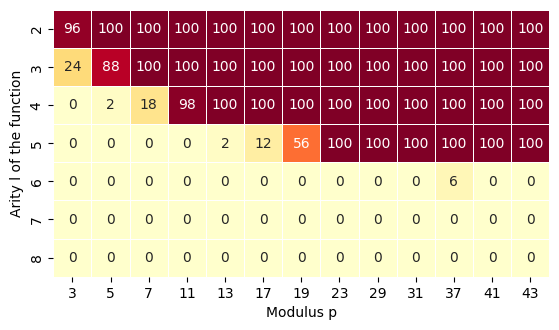
\includegraphics[]{img/p_encodings/heatmap_success.png}
    \caption{Rate of success of the algorithm for 100 random Boolean functions for different values of $\ell$ and $p$.}
    \label{fig:heatmap_success}
\end{figure}


Figure \ref{fig:lineplot_timings} shows the evolution of the time of execution of the algorithm for random Boolean functions \emph{for which no solution exists}.  It shows the explosion of the complexity for high values of
$p$, and justifies the need of a more efficient algorithm for those function (we introduce one in Section \ref{sec:graphs}).  


\TODO{Harmoniser l'algorithme suivant (commenté)}
\begin{figure}
    \centering
    \begin{minipage}{0.55\textwidth}
        \centering
        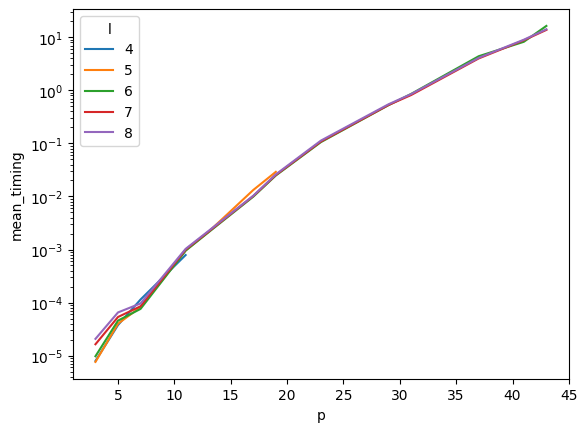
\includegraphics[width=\linewidth]{img/p_encodings/lineplot_timings.png}
        \caption{Running time of the algorithm for different values of $\ell$ and $p$ for random functions. Note that the scale is logarithmic.}        
        \label{fig:lineplot_timings}
        \end{minipage}\hspace{0.04\textwidth}
    \begin{minipage}{0.35\textwidth}
        \centering
        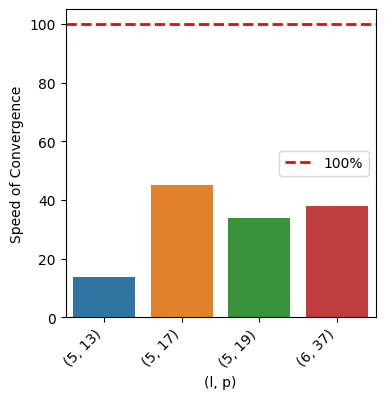
\includegraphics[width=\linewidth]{img/p_encodings/barplot.png}
        \caption{Ratio between the time to find a solution when it exists with the time to run the full algorithm when no solution exists.}
        \label{fig:barplot_ratio}
    \end{minipage}
    \caption{Some metrics about running time.}
    \label{fig:overall}
\end{figure}
Lastly, Figure \ref{fig:barplot_ratio} shows how long it takes to find a solution when one exists, relatively to the running time when no solution exist at all. It illustrates a form of "speed of convergence" and shows that it is located around $\frac{1}{3}$.



    
\subsection{An Efficient Sieving Heuristic to Find Suitable Encodings}
\label{sec:heuristic_matthieu}


Let us consider a function $f: \B^\ell \mapsto \B$ of matrix of constraints $C=(C_j^{(i)})_{\substack{1 \le i \le n_j\\1 \le j \le \ell}}$ and its associated system of linear inequalities:

$$
\left \{
\begin{array}{c}
     c_1^{(1)} \times d_1 + c_2^{(1)} \times d_2 + \dots + c_\ell^{(1)} \times d_\ell   \neq 0 \mod p\\
     c_1^{(2)} \times d_1 + c_2^{(2)} \times d_2 + \dots + c_\ell^{(2)} \times d_\ell \neq 0 \mod p\\
    \dots
\end{array}
\right .
$$


The principle is to sample random values in $\Z$ (with some large bound) and affect them to the $d_j$'s. If all the corresponding values for all the $C_i = \sum_{j=1}^{\ell} c_j^{(i)} \times d_j$ are not divisible by a value $p$, then the vector $(d_j \mod p \mid j \in \{1, \dots, \ell\})$ is a solution of the system of inequalities generated by $C$. 


To reduce the amount of samples required to find a solution, we want to avoid sampling trivially wrong sets of $d_j$'s. For example, if all the $d_j$'s are themselves divisible by $p$, then the $C_i$'s will all be divisible as well. To tackle this problem, we perform the sampling across \emph{prime numbers in $\Z$}.



%\begin{algorithm}
%    \caption{Sample a solution $\vec d$ in $\Z$ for a function $f$ and returns a possible value for $p$.}
%    \label{alg:heuristic_matthieu}
%    \begin{algorithmic}
%    \Require \\
%    $\{C_i\}_{1 \le i \le n}$ \Comment{The lines of the matrix of constraints $C$ of the function $f$ } \newline
%    $P$ \Comment{The sets of possible values for $p$ to be tested} \newline
%    $D$ \Comment{The sets of possible values in $\Z$ to assign to the $d_i$'s. All these elements are big primes}
%    \Ensure $f$ is possible to evaluate using a modulus smaller or equal than $p$.
%    \State{$\vec{d} \drawfrom D$} \Comment{Sample random prime values in $\Z$ and assign it to $\Vec{d} = (d_1, \dots, d_l)$}
%    \State{$\vec r = C \times \vec{d}$}  \Comment{$\vec r$ is the right member of the system}
%    \For {$p \in P$}
%        \If{$0 \in [\Vec{r}]_p$}          \Comment{If $p$ divides one of the coordinates of $\vec r$}
%            \State{$P \gets P \setminus \{p\}$} \Comment{This value of $p$ is incorrect}
%        \EndIf
%    \EndFor
%    \If{$\mid P \mid > 0$}
%        \State{\Return{$\min(P)$}} \Comment{Returns the smallest possible value for $p$, if any.}
%    \EndIf   
%    \end{algorithmic}
%\end{algorithm}


Running this algorithm several times and keeping the smallest returned value for $p$, one gets an upper bound on the minimum $p$ required to evaluate a function with our framework. Note that, on the contrary of the deterministic search algorithm, this heuristic does not require a prime $p$.


\paragraph{Example:} Let us consider the s-box of the block cipher ASCON. We study this s-box in more details and provide an exact optimized solution for its homomorphic evaluation in Section \ref{sec:ascon}. Here, we apply Algorithm \ref{alg:heuristic_matthieu} on the five functions generating the five output bits and monitor the results until we gather $N=10000$ non-zero possible values for $p$.


The figure \ref{fig:ascon_0_p_frequencies} shows the repartition of the returned values of $p$ by the algorithm during these $N$ runs on the first subfunction. The optimal value of $p$ found by the deterministic approach of Section \ref{sec:search_algorithm} is $17$ so the upper bound $19$ is pretty close, despite being rarely found by the algorithm. Also, the figure \ref{fig:ascon_0_count_iter} shows $21$ (the second best solution found by the sieving) is almost instantly found by the algorithm.


\begin{figure}
  \begin{minipage}{0.48\linewidth}
    \    \centering
    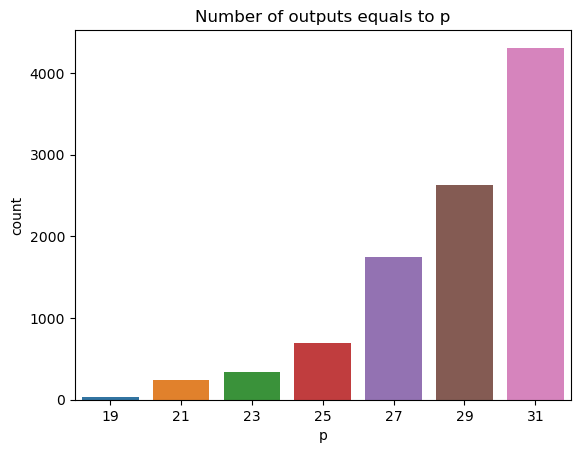
\includegraphics[width=\linewidth]{img/p_encodings/heuristic_ascon_0_p_frequencies.png}
    \caption{The outputs of $10000$ runs of the Algorithm \ref{alg:heuristic_matthieu} for the first subfunction of the Ascon s-box}
    \label{fig:ascon_0_p_frequencies}
  \end{minipage} \hfill
  \begin{minipage}{0.48\linewidth}
    \centering
    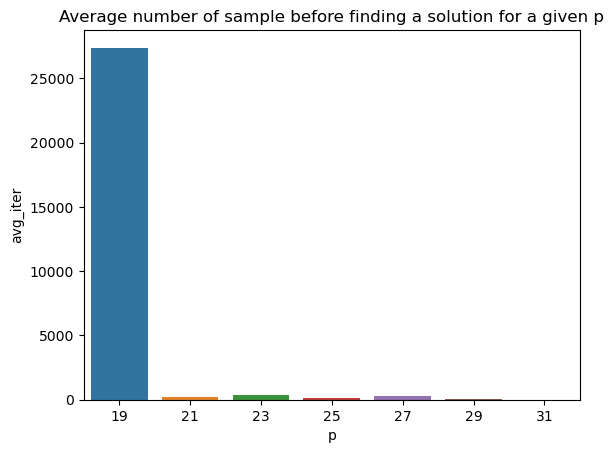
\includegraphics[width=\linewidth]{img/p_encodings/heuristric_ascon_0_count_iter.png}
    \caption{Number of iterations required to get a solution for a given value of $p$}
    \label{fig:ascon_0_count_iter}
  \end{minipage}
\end{figure}


In the process of finding the smallest $p$ possible and a correct vector of $p$-encoding to evaluate a function $f$, this heuristic is really efficient to get a tight upper bound on the value of $p$.



